%%%%%%%%%%%%%%%%%%%%%%%%%%%%%%%%%%%%%%%%%%%%%%%%%%%
%
%  New template code for TAMU Theses and Dissertations starting Fall 2012.  
%  For more info about this template or the 
%  TAMU LaTeX User's Group, see http://www.howdy.me/.
%
%  Author: Wendy Lynn Turner 
%	 Version 1.0 
%  Last updated 8/5/2012
%
%%%%%%%%%%%%%%%%%%%%%%%%%%%%%%%%%%%%%%%%%%%%%%%%%%%

%%%%%%%%%%%%%%%%%%%%%%%%%%%%%%%%%%%%%%%%%%%%%%%%%%%%%%%%%%%%%%%%%%%%%%%
%%%                           SECTION II
%%%%%%%%%%%%%%%%%%%%%%%%%%%%%%%%%%%%%%%%%%%%%%%%%%%%%%%%%%%%%%%%%%%%%%

\chapter{\uppercase {Application of the entropy viscosity method to the multi-D Euler equations with variable area:}}\label{chap:euler}
%%%%%%%%%%%%%%%%%%%%%%%%%%%%%%%%%%%%%%%%%%%%%%%%%%%%%%%%%%%%%
%%%%%%%%%%%%%%%%%%%%%%%%%%%%%%%%%%%%%%%%%%%%%%%%%%%%%%%%%%%%%
\section{Introduction} \label{sec:intro}
%%%%%%%%%%%%%%%%%%%%%%%%%%%%%%%%%%%%%%%%%%%%%%%%%%%%%%%%%%%%%%%%%%%%%%%%%%%%%%%%%%%%%%%%%%%%%%%%%%%%
%%%%%%%%%%%%%%%%%%%%%%%%%%%%%%%%%%%%%%%%%%%%%%%%%%%%%%%%%%%%%%%%%%%%%%%%%%%%%%%%%%%%%%%%%%%%%%%%%%%%
Over the past years an increasing interest raised for computational methods that can solve both compressible and incompressible flows. In engineering applications, there is often the need to solve for complex flows where a near incompressible regime or low Mach flow coexists with a supersonic flow domain. For example, such flow are encountered in aerodynamic in the study of airships. In the nuclear industry, flows are nearly the incompressible regime but compressible effects cannot be neglected because of the heat source and thus needs to be accurately resolved. \\
When solving the multi-D Euler equations for a wide range of Mach numbers, multiple problems have to address: stability, accuracy and acceleration of the convergence in the low Mach regime. Because of the hyperbolic nature of the equations, shocks can form during transonic and supersonic flows, and require the use of the numerical methods in order to stabilize the scheme and correctly resolve the discontinuities. The literature offers a wide range of stabilization methods: flux-limiter \cite{FluxLimiter, FluxLimiter2}, pressure-based viscosity method (\cite{PBV_book}), Lapidus method (\cite{Lapidus_paper, LMP, Lapidus_book}), and the entropy-viscosity method(\cite{jlg1, jlg2}) among others. These numerical methods are usually developed using simple equation of states and tested for transonic and supersonic flows where the disparity between the acoustic waves and the fluid speed is not large since the Mach number is of order one. This approach leads to a well-known accuracy problem in the low Mach regime where the fluid velocity is smaller that the speed of sound by multiple order of magnitude. The numerical dissipative terms become ill-scaled in the low Mach regime and lead to the wrong numerical solution by changing the nature of the equations solved. This behavior is well documented in the literature \cite{LowMach1, LowMach2, LowMach3} and often treated by performing a low Mach asymptotic study of the multi-D Euler equation. This method was originally used \cite{LowMach1} to show convergence of the compressible multi-D Euler equations to the incompressible ones. Thus, by using the same method, the effect of the dissipative terms in the low Mach regime, can be understood and, when needed, a fix is developed in order to ensure the convergence of the equations to the correct physical solution. This approach was used as a fixing method for multiple well known stabilization methods alike Roe scheme (\cite{Roe}) and SUPG \cite{LowMach3} while preserving the original stabilization properties of shocks.  \\
We propose, through this paper, to investigate how the entropy viscosity method, when applied to the multi-D Euler equations with variable area, behaves in the low Mach regime. This method was initially introduced by Guermond et al. to solve for the hyperbolic systems and has shown good results when used for solving the multi-D Euler equations with various discretization schemes. More importantly, it is simple to implement, can be used with unstructured grids,  and its dissipative terms are consistent with the entropy minimum principle and proven valid for any equation of state under certain conditions \cite{jlg}. \\

%This paper is organized as follows: in \sect{sec:entro_visc} the current definition of the entropy viscosity method is recalled, and inconsistency with the low Mach regime are pointed out. Since our interest is in the variable area version of the multi-D Euler equation, the reader is guided trough the steps leading to the derivation of the dissipative terms on the model of \cite{jlg}. Then in \sect{sec:extension}, a new definition of the viscosity coefficient is introduced and derived from a low Mach asymptotic study. After detailing the spatial and temporal discretization method in \sect{sec:solution_tech}, 1-D and 2-D numerical results are presented in \sect{sec:results} for a wide range of Mach numbers: low Mach flow over a cylinder and a circular bump, and supersonic flow in a compression corner \cite{CompressionCorner}. Convergence studies are performed in 1-D, in order to demonstrate the accuracy of the solution. \\

% keep this as a comment for now
%\tcr{I wouldn't recall this here. Let me think about that.}\\
%For purpose of clarity, the multi-D Euler equations with variable area are recalled in \eqt{eq:euler_eq} and the corresponding variables are defined:
%%
%\begin{equation}
%\label{eq:euler_eq}
%\left\{ 
%\begin{array}{lll}
%\partial_t \left( \rho A\right) + \div \left( \rho \vec{u} A\right) = 0\\
%\partial_t \left( \rho \vec{u} A\right) + \div \left[ \left( \rho \vec{u} \otimes \vec{u} + P \mathbf{I} \right) A \right] = P \grad A\\
%\partial_t \left( \rho E A\right) + \div \left[ \vec{u} \left( \rho E + P \right) A\right] = 0 \\
%P = P\left( \rho, e \right)
%\end{array}
%\right.
%\end{equation}

%%%%%%%%%%%%%%%%%%%%%%%%%%%%%%%%%%%%%%%%%%%%%%%%%%%%%%%%%%%%%%%%%%%%%%%%%%%%%%%%%%%%%%%%%%%%%%%%%%%%
%%%%%%%%%%%%%%%%%%%%%%%%%%%%%%%%%%%%%%%%%%%%%%%%%%%%%%%%%%%%%%%%%%%%%%%%%%%%%%%%%%%%%%%%%%%%%%%%%%%%
\section{The Entropy Viscosity Method} \label{sec:entro_visc}
%%%%%%%%%%%%%%%%%%%%%%%%%%%%%%%%%%%%%%%%%%%%%%%%%%%%%%%%%%%%%%%%%%%%%%%%%%%%%%%%%%%%%%%%%%%%%%%%%%%%
%%%%%%%%%%%%%%%%%%%%%%%%%%%%%%%%%%%%%%%%%%%%%%%%%%%%%%%%%%%%%%%%%%%%%%%%%%%%%%%%%%%%%%%%%%%%%%%%%%%%

%===================================================================================================
\subsection{Background} \label{sec:background}
%===================================================================================================

The Euler equations are given by
\begin{subequations}
\label{eq:euler_eq}
%
\begin{equation}
\partial_t \rho  + \div \left( \rho \vec{u} \right) = 0
\end{equation}
%
\begin{equation}
\partial_t \left( \rho \vec{u} \right) + \div \left( \rho \vec{u} \otimes \vec{u} + P \mathbb{I} \right) = 0 
\end{equation}
%
\begin{equation}
\partial_t \left( \rho E \right) + \div \left[ \vec{u} \left( \rho E + P \right) \right] = 0
\end{equation}
\end{subequations}
%
where $\rho$, $\rho \vec{u}$ and $\rho E$ are the density, the momentum and the total energy, respectively, and will be referred to as the conservative variables. $\vec{u}$ is the fluid velocity and its specific internal energy is denoted by $e=E-\tfrac{u^2}{2}$. An equation of state, dependent upon $\rho$ and $e$, is used to compute the pressure $P$. The tensor product $\vec{a} \otimes \vec{b}$ is such that $(\vec{a} \otimes \vec{b})_{i,j} = a_i b_j$. The identity tensor is denoted by $\mathbb{I}$.

Next, the entropy viscosity method \cite{jlg1, jlg2, jlg3, valentin} applied to \eqt{eq:euler_eq} is recalled. The method consists of adding dissipative terms with a viscosity coefficient modulated by the entropy production; this allows for a high-order accuracy when the solution is smooth (provided that the spatial and temporal discretizations also are high order). 
The derivation of the viscous regularization (or dissipative terms) is carried out to be consistent with the entropy minimum principle; details and proofs of the derivation can be found in \cite{jlg}. The viscous regularization thus obtained is valid for any equation of state as long as the physical entropy function $s$ is such that $-s$ is a convex function with respect to the internal energy $e$ and the specific volume $1/\rho$. Euler equations with viscous regularization are given in \eqt{eq:euler_visc}:
%
\begin{subequations}
\label{eq:euler_visc}
%
\begin{equation}
\partial_t \rho  + \div \left( \rho \vec{u} \right) = \div \left( \kappa \grad \rho \right) 
\end{equation}
%
\begin{equation}
\partial_t \left( \rho \vec{u} \right) + \div \left( \rho \vec{u} \otimes \vec{u} + P \mathbf{I} \right) = \div \left( \mu \rho \grad^s \vec{u}  + \kappa \vec{u} \otimes \grad \rho \right)  
\end{equation}
%
\begin{equation}
\partial_t \left( \rho E \right) + \div \left[ \vec{u} \left( \rho E + P \right) \right] = \div \left( \kappa \grad \left( \rho e \right) + \frac{1}{2}|| \vec{u} ||^2 \kappa \grad \rho +  \rho \mu \vec{u} \grad \vec{u}  \right) 
\end{equation}
\end{subequations}
%
where $\kappa$ and $\mu$ are positive viscosity coefficients. $\grad^s \vec{u}$ denotes the symmetric gradient operator that guarantees the method to be rotationally invariant \cite{jlg}. The viscosity coefficients are key ingredients in the viscous regularization of \eqt{eq:euler_visc}.  
Other stabilization approaches have been proposed in the literature, for instance, the Lapidus method \cite{Lapidus_book, Lapidus_paper} or pressure-based viscosity methods \cite{PBV_book}. Here, we follow the work of Guermond et al. and define the viscosity coefficients, $\kappa$ and $\mu$, based on the local entropy production. These coefficients are numerically evaluated using the local entropy residual $\resi(\vec{r},t)$ defined in \eqt{eq:ent_residual}; $\resi(\vec{r},t)$ is known to be peaked in shocks and vanishingly small elsewhere \cite{Toro}. 
%
\begin{equation}
\label{eq:ent_residual}
\resi(\vec{r}, t) := \partial_t s + \vec{u} \cdot \grad s
\end{equation}
%
In the current version of the method, the ratio of $\kappa$ to $\mu$ is defined as a numerical Prandlt number, $\Pr = \kappa / \mu$.  $\Pr$ is a user-defined parameter and is usually taken in the range $[ 0.001; 1 ]$. Since the entropy residual $\resi(\vec{r},t)$ may be extremely large in shocks, the definition of the viscosity coefficients also includes a first-order viscosity coefficient that serves as upper bound for the entropy-based viscosity coefficients. The first-order viscosity coefficients, denoted by $\mu_{\max}$ and $\kappa_{\max}$, are chosen so that the numerical scheme becomes equivalent to the upwind scheme when the first-order coefficients are employed. The upwind scheme is known to be over-dissipative but guarantees monotonicity \cite{Toro}. In practice, the viscosity coefficients only saturate to the first-order viscosity coefficients in shocks and are much smaller elsewhere, hence avoiding over-dissipation due to the upwind method.  The first-order viscosity coefficients $\mu_{\max}$ and $\kappa_{\max}$ are equal and set proportional to the largest local eigenvalue $|| \vec{u} || + c $:
%
\begin{equation}
\label{eq:fo}
\mu_{\max}(\vec{r}, t) = \kappa_{\max}(\vec{r}, t) = \frac{h}{2} \left( || \vec{u}(\vec{t,r}) || + c(\vec{t,r}) \right),
\end{equation}
%
where $h$ denotes the local grid size (for higher than linear finite element representations, $h$ is defined as the ratio of the grid size to the polynomial order of the test functions used, see Eq. 2.4 in \cite{valentin}). For simplicity, the first-order viscosity coefficient will only be referred to as the $\kappa_{\max}(\vec{r}, t)$. In practice, these quantities are evaluated within a given cell $K$ at quadrature points:
%
\begin{equation}
\label{eq:fo_quad}
\kappa^K_{\max}(\vec{r}_q, t) = \frac{h_K}{2} \left( || \vec{u}(\vec{t,r_q}) || + c(\vec{t,r_q}) \right),
\end{equation}
%
where $\vec{r}_q$ denotes the position of a quadrature point.
As stated earlier, the entropy viscosity coefficients, which we denote by $\kappa_e$ and $\mu_e$, are set proportional to the entropy production evaluated by computing the local entropy residual $\resi$. The definitions also include the inter-element jump of the entropy flux $J[s]$, % that is also a good entropy production indicator, thus 
allowing for the detection of discontinuities other than shocks \tcr{(e.g., contact)}.
%
\begin{subequations}
\label{eq:ent_visc_coeff}
\begin{equation}
\mu^K_e(\vec{r}_q,t) =  h_K^2 \frac{\max\left( | \resi^K(\vec{r}_q,t) |, J^K[s](t) \right)}{|| s - \bar{s} ||_\infty}  
\end{equation}
\begin{equation}
\kappa^K_e(\vec{r}_q,t) = Pr \, \mu^K_e(\vec{r}_q,t)
\end{equation}
\end{subequations}
%
where $|| \cdot ||_\infty$ and $\bar{\cdot}$ denote the L$_\infty$-norm and the average operator over the entire computational domain, respectively. The definition of the entropy jump $J[s]$ is spatial discretization-dependent and examples of definitions can be found in \cite{valentin} for discontinuous Galerkin discretization. For continuous finite element methods (FEM), the jump of a given quantity is defined as the inter-element change in its normal derivative ($\partial_n = \grad \cdot \vec{n}$) along the common face separating the two elements. We take the largest value over all faces $f$ present on the boundary $\partial K$ of element $K$:
%
\begin{equation}
\label{eq:jump_CFEM}
J^K[s](t) = \max_{f\in\partial K}  \max_{\vec{r}_q \in f} \jmp{\grad s(\vec{r}_q,t) \cdot \vec{n}(\vec{r}_q) }_f \, ,
\end{equation}
%
where $\jmp{a(\vec{r}_q)}_f$ denotes the inter-element jump in $a(\vec{r})$ at quadrature point $\vec{r}_q$ on face $f$.  
The denominator $|| s - \bar{s} ||_\infty$ is used for dimensionality purposes.
% \tcr{and should not be of the same order as $h$, on penalty of loosing the high-order accuracy} \tcb{you do not like this?}. 
Currently, there are no theoretical justification for choosing the denominator beyond a dimensionality argument. 
Finally, the viscosity coefficients $\mu$ and $\kappa$ are as follows:
%
\begin{equation}
\mu(\vec{r},t)    = \min\Big( \mu_e(\vec{r},t)   \,,\, \mu_{\max}(\vec{r},t)    \Big) 
\quad \text{ and } \quad 
\kappa(\vec{r},t) = \min\Big( \kappa_e(\vec{r},t)\,,\, \kappa_{\max}(\vec{r},t) \Big).
\end{equation}
%
Given these definitions, we have the following properties.
In shock regions, the entropy viscosity coefficients will experience a peak because of entropy production and thus will saturate to the first-order viscosity. The first-order coefficients are known to be over-dissipative and will smooth out any oscillatory behavior. Elsewhere in the domain, entropy production will be small and the viscosity coefficients $\mu$ and $\kappa$ will remain small. % and of order $h^2$.
High-order accuracy for entropy-based viscous stabilization was demonstrated using several 1-D shock tube examples and various 2-D tests \cite{jlg1, jlg2, valentin}.

%===================================================================================================
\subsection{Issues in the Low-Mach Regime} 
%===================================================================================================

In the low-Mach Regime, the flow is known to be isentropic, resulting in very little entropy production. Since the entropy viscosity method is directly based on the evaluation of the local entropy production, it is of interest to study how the entropy viscosity coefficients $\mu_e$ and $\kappa_e$ scale in the low-Mach regime. In practice, the entropy residual $\resi$ will be very small in that regime and so will be the denominator $|| s - \bar{s} ||_\infty$, thus making the definition of the viscosity coefficients in \eqt{eq:ent_visc_coeff} undetermined and likely ill-scaled.  One possible approach would consist of expanding the numerator and denominator in terms of the Mach number and deriving its limit when the Mach number goes to zero. Such derivation may not be straightforward, especially for general equations of state. However, this can be avoided by noting that the entropy residual $\resi$ can be recast as a function of pressure, density, velocity, and speed of sound as shown in \eqt{eq:ent_res} of \sect{sec:new_ent_prod}. This alternate entropy residual definition is the basis for the low-Mach analysis carried out in this paper and possesses several advantages that are detailed next. %in \sect{sec:new_ent_prod}.

%%%%%%%%%%%%%%%%%%%%%%%%%%%%%%%%%%%%%%%%%%%%%%%%%%%%%%%%%%%%%%%%%%%%%%%%%%%%%%%%%%%%%%%%%%%%%%%%%%%%
%%%%%%%%%%%%%%%%%%%%%%%%%%%%%%%%%%%%%%%%%%%%%%%%%%%%%%%%%%%%%%%%%%%%%%%%%%%%%%%%%%%%%%%%%%%%%%%%%%%%
\section{An All-speed Reformulation of the Entropy Viscosity Method} \label{sec:extension}
%%%%%%%%%%%%%%%%%%%%%%%%%%%%%%%%%%%%%%%%%%%%%%%%%%%%%%%%%%%%%%%%%%%%%%%%%%%%%%%%%%%%%%%%%%%%%%%%%%%%
%%%%%%%%%%%%%%%%%%%%%%%%%%%%%%%%%%%%%%%%%%%%%%%%%%%%%%%%%%%%%%%%%%%%%%%%%%%%%%%%%%%%%%%%%%%%%%%%%%%%

In this section, the entropy residual $\resi$ is recast as a function of pressure, density, velocity and speed of sound. Then, a low-Mach asymptotic study is carried out for the Euler equations with viscous regularization in order to derive an appropriate normalization parameter that is valid in the low-Mach regime as well as for transonic and supersonic flows. 

%===================================================================================================
\subsection{New Definition of the Entropy Production Residual}\label{sec:new_ent_prod} 
%===================================================================================================

The first step in defining viscosity coefficients that behave well in the low-Mach limit is to recast the entropy residual in terms of thermodynamic variables. This provides physical insight on possible normalization choices that can be valid in both low-Mach and transonic flows. The alternate definition of the entropy residual is given in \eqt{eq:ent_res}. The derivation that leads to this equation is provided in \app{app:ent_res}. 
%
\begin{equation}
\label{eq:ent_res}
\resi(\vec{r},t) := \partial_t s + \vec{u} \cdot \grad s = \matder{s} = \frac{s_e}{P_e} \left( \underbrace{\matder{P} - c^2 \matder{\rho} }_{\resinew(\vec{r},t)} \right) ,
\end{equation} 
%
where $\matder{\ }$ denotes the material derivative ($\matder{\ }:= \frac{\partial}{\partial t} + \vec{u} \cdot \grad$), and $x_y$ is the standard shortcut notation for the partial derivative of $x$ with respect to $y$, e.g., $P_e:=\frac{\partial P}{\partial e}$. 
%
The entropy residuals $\resi$ and $\resinew$ are proportional to one another and will experience similar variations in space and time. Thus, one may elect to employ $\resinew$ instead of $\resi$ for the evaluation of the local entropy residual. The new expression presents several advantages:
%
\begin{itemize}
\item an analytical expression of the entropy function $s$ is no longer needed: the residual $\resinew$ is evaluated using the local values of pressure, density, velocity and speed of sound. Deriving an entropy function for some complex equation of states may be difficult;
\item suitable normalizations for the residual $\resinew$ can be devised. Examples include the pressure itself or combinations of the density, the speed of sound and the norm of the velocity, i.e., $\rho c^2$, $\rho c || \vec{u} ||$ or $\rho || \vec{u} ||^2$. 
\end{itemize}
%
Denoting the normalization of $\resinew$ by $\norm_P$, the entropy-based viscosity coefficients $\mu_e$ and $\kappa_e$ can be re-defined as follows:
%
\begin{subequations}
\label{eq:visc_definition}
\begin{equation}
\mu^K_e(\vec{r},t)    = h_K^2 \frac{\max\left( | \resinew^K(\vec{r}_q,t) |\,, || \vec{u}(\vec{r}_q,t) || J^K[P](t) \,, || \vec{u}(\vec{r}_q,t) c^2(\vec{r}_q,t) || J^K[\rho](t) \right)}{\norm_P^\mu}    \, ,
\end{equation} 
\text{and} 
\begin{equation}
\kappa^K_e(\vec{r},t) = h_K^2 \frac{\max\left( | \resinew^K(\vec{r}_q,t) |\,, || \vec{u}(\vec{r}_q,t) || J^K[P](t) \,, || \vec{u}(\vec{r}_q,t) c^2(\vec{r}_q,t) || J^K[\rho](t) \right)}{\norm_P^\kappa} \, .
\end{equation}
\end{subequations}
%
Note that now the jump operator acts on the variables appearing in $\resinew$, namely, pressure and density. The $\mu$ and $\kappa$ coefficients are kinematic viscosities (units of $m^2/s$); the normalization parameters $\norm_P$ are thus in units of pressure, hence the use of the subscript $P$.  Note also that we are not requiring the same normalization for both $\mu_e$ and $\kappa_e$ so the entropy viscosity coefficients can be different. The low-Mach asymptotic study presented next will determine the proper normalization.

%===================================================================================================
\subsection{Asymptotic Study in the Low-Mach Regime} \label{sec:lowMach}
%\tcb{What about: Derivation of the all-speed reformulation of the viscosity coefficients}
%===================================================================================================

The Euler equations with viscous stabilization, \eqt{eq:ent_visc_coeff}, bear some similarities with the Navier-Stokes equations in the sense that dissipative terms (containing second-order spatial derivatives) are present in both sets of equations. An abundant literature exists regarding the low-Mach asymptotics of the Navier-Stokes equations \cite{LowMach1, LowMach2, LowMach3, Muller}.   
%
The asymptotic study presented here is inspired by the work of Muller et al. \cite{Muller} where an asymptotic derivation for the Navier-Stokes was presented. 
We remind the reader that the objective is to determine appropriate scaling for the entropy viscosity coefficients so that the dissipative terms remain well-scaled for two limit cases: 
(i) the isentropic limit where Euler equations degenerate to an incompressible system of equations in the low-Mach limit and 
(ii) the non-isentropic limit with formation of shocks. 
The isentropic limit of Euler equations with viscous regularization should yield the incompressible fluid flows results in the low-Mach limit, namely, that the pressure fluctuations are of the order $M^2$ and that the velocity satisfies the divergent constraint $\div \vec{u}_0 = 0$ \cite{LowMach1, LowMach2, LowMach3}. For non-isentropic situations, shocks may form for any value of Mach number and the minimum entropy principle should still be verified so that numerical oscillations, if any, be controlled by the entropy viscosity method independently of the value of the Mach number.
Our objective is to determine the appropriate scaling for the Reynolds and P\'eclet numbers, $\Re_\infty$ and $\Pe_\infty$, in these two limit cases.

In this Section, we are interested in the isentropic limit, the non-isentropic case is treated later.
% where Euler equations degenerate to an incompressible system of equations.
% The scaling of the Prandtl number defined in the original definition of the entropy viscosity method as recalled in \sect{sec:background} will be also demonstrated. 
%It will be also showed that the Prandlt number defined in the original definition of the entropy viscosity method as recalled in \sect{sec:background}, has to scale as the inverse of the Mach number square in order to have well-scale dissipative terms. \tcr{I need to think a bit more about the previous sentences}
%
The first step in the study of the limit cases (i) and (ii) is to re-write \eqt{eq:euler_visc} in a non-dimensional manner. In order to do so, the following variables are introduced:
%
\begin{multline}
\label{eq:norm_param}
\rho^*   = \frac{\rho}{\rho_\infty}           ,\
u^*      = \frac{u}{u_\infty}                 ,\
P^*      = \frac{P}{\rho_\infty c^2_\infty}   ,\
E^*      = \frac{E}{c^2_\infty }              ,\\
x^* = \frac{x}{L_\infty}                      ,\
t^* = \frac{t}{L_\infty / u_\infty}           ,\ 
\mu^*    = \frac{\mu}{\mu_\infty}             ,\
\kappa^* = \frac{\kappa}{\kappa_\infty}       ,
\end{multline}
%
where  the subscript $\infty$ denote the far-field or stagnation quantities and the superscript $*$ stands for the adimensional variables. The far-field reference quantities are chosen such that the dimensionless flow quantities are of order 1. The reference Mach number is given by
%
\begin{equation}
M_\infty = \frac{u_\infty}{c_\infty} ,
\end{equation}
%
where $c_\infty$ is a reference value for the speed of sound. Then, the scaled Euler equations with viscous regularization are:
%
\begin{subequations} 
\label{eq:Euler_eq2}
%
\begin{equation}
\label{eq:euler_eq2_cont}
\partial_{t^*} \rho^*+ \divv{*}  \left(  \rho^* \vec{u}^*  \right) = \frac{1}{\Pe_\infty} \divv{*}  ( \kappa^* \gradd{*} \rho^* )
\end{equation}
%
\begin{multline}
\label{eq:euler_eq2_mom}
\partial_{t^*} \left( \rho^* \vec{u}^* \right) 
+ \divv{*} \left( \rho^* \vec{u}^*\otimes \vec{u}^* \right) 
+ \frac{1}{M_\infty^2}\gradd{*}  P^*  
= 
\frac{1}{\Re_\infty} \divv{*} \left( \rho^* \mu^* \gradd{s,*} \vec{u}^* \right)  \\
+
\frac{1}{\Pe_\infty} \divv{*} \left(\vec{u}^*\otimes \kappa^* \gradd{*}  \rho^* \right)
\end{multline}
%
\begin{multline}
\label{eq:euler_eq2_energy}
\partial_{t^*} \left( \rho^* E^* \right) 
+ \divv{*}  \left[ \vec{u}^* \left( \rho^* E^* + P^* \right) \right] 
=
\frac{1}{\Pe_\infty} \divv{*}  \left( \kappa^*  \gradd{*} (\rho^* e^*) \right)   \\
+
\frac{M_\infty^2}{\Re_\infty} \divv{*}  \left( \vec{u}^* \rho^* \mu^* \gradd{s,*} \vec{u}^* \right)
+ 
\frac{M_\infty^2}{2 \Pe_\infty} \divv{*}  \left(\kappa^* (u^*)^2 \gradd{*} \rho^* \right) \, ,
\end{multline}
%
\end{subequations}
where the numerical Reynolds $(\Re_\infty)$ and P\'eclet $(\Pe_\infty)$ numbers are defined as follows:
%
\begin{equation}
\label{eq:ref_numb}
\Re_\infty = \frac{u_\infty L_\infty}{\mu_\infty} \text{ and }
\Pe_\infty = \frac{u_\infty L_\infty}{\kappa_\infty} \, .
\end{equation}
%
Note that the Prandlt number used in the original version of the entropy viscosity method is simply given by 
\begin{equation} \label{eq:ref_nb_pr} 
\Pr_\infty = \Pe_\infty / \Re_\infty \, .
\end{equation}
For simplicity, we use here the ideal gas equation of state; its non-dimensionalized expression is given by
%
\begin{equation}
\label{eq:euler_eq2_eos}
P^* = \left( \gamma-1 \right) \rho^*\left(  E^* -\frac{1}{2} M_\infty^2 (u^*)^2 \right) = \left( \gamma-1 \right) \rho^* e^* \, .
\end{equation}
%\tcb{this assumption is only useful in the asymptotic limit. I believe it is possible to carry the same asymptotic limit by assuming a more generic form of the equation of state such as $P = f(\rho)$ for isentropic flow. Do you think it is a good idea to do so?}\\
%
The numerical Reynolds and P\'eclet numbers defined in \eqt{eq:ref_numb} are related to the entropy viscosity coefficients $\mu_\infty$ and $\kappa_\infty$. Thus, once a scaling (in powers of $M_\infty$) is obtained for $\Re_\infty$ and $\Pe_\infty$, the corresponding normalization parameters $\norm_P^\mu$ and $\norm_P^\kappa$ will automatically be set. 
For brevity, the superscripts $^*$ are omitted in the remainder of this section. 

%We consider two limit cases: isentropic flows \tcr{(the low-Mach asymptotic limit)} and non-isentropic situations (both subsonic and supersonic since we do not wish to specialize the entropy viscosity method to only low-Mach flows). 

%\tcr{? so that shocks are stabilized and the isentropic incompressible limit and its main features are preserved.}
%so that the main features of the incompressible fluid equations are retrieved in the low-Mach limit, \tcb{and shock can be efficiently stabilized}.

In the low-Mach isentropic limit, shocks cannot form and the compressible Euler equations are known to converge to the incompressible equations when the Mach number tends to zero. When adding dissipative terms, as is the case with the entropy viscosity method, the main properties of the low-Mach asymptotic limit have to be preserved.
We begin by expanding each variable in powers of the Mach number. As an example, the expansion for the pressure is given by:
%
\begin{equation}
\label{eq:expansion}
P(\vec{r}, t) = P_0(\vec{r}, t) + P_1(\vec{r}, t) M_\infty + P_2(\vec{r}, t) M_\infty^2 + \dots 
\end{equation}
%
By studying the resulting momentum equations for various powers of $M_\infty$, we observe the following: the leading order and first-order pressure terms, $P_0$ and $P_1$, are spatially constant if and only if $\Re_\infty = \Pe_\infty = 1$. In this case, we have, 
\begin{subequations}\label{eq:asympt_equ1}
at order $M_\infty^{-2}$:
\begin{equation}
\label{eq:asympt_equ1_cont}
\grad P_0 = 0
\end{equation}
%
and, at order $M_\infty^{-1}$,
\begin{equation}
\label{eq:asympt_equ1_mom}
\grad P_1 = 0 \, .
\end{equation}
\end{subequations}
%
Using the scaling $\Re_\infty = \Pe_\infty = 1$, the leading-order expressions for the continuity, momentum, and energy equations are:
\begin{subequations}
\label{eq:asympt_equ2}
%
\begin{equation}
\label{eq:asympt_equ2_cont}
 \partial_t \rho_0 + \div ( \rho \vec{u} )_0 = \div ( \kappa \grad \rho )_0
\end{equation}
%
\begin{equation}
\label{eq:asympt_equ2_mom}
\partial_t (\rho \vec{u})_0 + \div ( \rho \vec{u} \otimes \vec{u})_0 + \grad P_2 = \div (\rho \mu \grad^s \vec{u} +\kappa \vec{u} \otimes \grad \rho )_0
\end{equation}
%
\begin{equation}
\label{eq:asympt_equ2_ener}
 \partial_t(\rho E)_0 + \div \left[ \vec{u} (\rho E + P) \right]_0 = \div(\kappa \grad(\rho e))_0
\end{equation}
%
\end{subequations}
%
where the notation $(fg)_0$ means that we only keep the 0$^{\text{th}}$ order terms in the product $fg$. The leading-order of the equation of state is given by 
\begin{equation}
\label{eq:leading_order_eos}
 P_0 = (\gamma - 1) (\rho E)_0 .
\end{equation}
%
Using \eqt{eq:leading_order_eos}, the energy equation can be recast as a function of the leading-order pressure, $P_0$, as follows:
%
\begin{equation}\label{eq:asympt_equ3_ener}
 \partial_t P_0 + \gamma \div \left( \vec{u} P \right)_0 =  \div(\kappa \grad(P))_0
\end{equation}
%
From \eqt{eq:asympt_equ1_cont}, we infer that $P_0$ is spatially constant. Thus, \eqt{eq:asympt_equ3_ener} becomes
%
\begin{equation}
\frac{1}{\gamma P_0} \frac{d P_0}{dt} = - \div \vec{u}_0 
\end{equation}
%
and, at steady state, we have
%
\begin{equation}
% \gamma P_0 \div  \vec{u}_0 = 0 \Rightarrow \div  \vec{u}_0 = 0.
 \div  \vec{u}_0 = 0 \, .
\end{equation}
%
That is, the leading-order of velocity is divergence-free. The same reasoning can be applied to the leading-order of the continuity equation (\eqt{eq:asympt_equ2_cont}) to show that the material derivative of the density is zero:
\begin{equation}
\matder{\rho_0} := \partial_t \rho_0 + \vec{u}_0 \cdot \div \rho_0 = 0 \, .
\end{equation}
%
Therefore, we conclude that by setting the Reynolds and P\'eclet numbers to one, the incompressible fluid results are retrieved in the low-Mach limit when employing the compressible Euler equations with viscous regularization terms present. In addition, the scaling of the Prandtl number can also be obtained using \eqt{eq:ref_nb_pr}, hence clarifying the use of the numerical Prandtl in the original entropy viscosity method \cite{jlg1}.

%===================================================================================================
\subsection{Scaling of $\Re_\infty$ and $\Pe_\infty$ for non-isentropic flows} \label{sec:nonisentropic}
%===================================================================================================

Next, we consider the non-isentropic case. Recall that even subsonic flows can present shocks (for instance, a step initial condition in the pressure will trigger shock formation, independently of the Mach number). The non-dimensionalized form of the Euler equations given in \eqt{eq:Euler_eq2} provides some insight on the dominant terms as a function of the Mach number. This is particular obvious in the momentum equation, \eqt{eq:euler_eq2_mom}, where the gradient of pressure is scaled by $1/M_\infty^2$. In the non-isentropic case, we no longer have $\frac{\grad P}{M_2}=\grad P_2$ and this pressure gradient term may need to be stabilized by some dissipative terms of the same scaling so as to prevent spurious oscillations from forming. This leads to the following three possible requirements regarding the non-dimensionalized Reynolds and P\'eclet numbers for non-isentropic flows: 
(a) $\Re_\infty = M_\infty^2$ and $\Pe_\infty = 1$,
(b) $\Re_\infty = 1$ and $\Pe_\infty = M_\infty^2$, or
(c) $\Re_\infty = \Pe_\infty = M_\infty^2$. 
%
Any of these choices will also affect the stabilization of the continuity and energy equations. For instance, using a P\'eclet number equal to $M_\infty^2$ may effectively stabilize the continuity equation in the shock region but this may also add an excessive amount of dissipation for subsonic flows at the location of the contact wave. Such a behavior may not be suitable for accuracy purpose, making options (b) and (c) inappropriate. The same reasoning, left to the reader, can be carried out for the energy equation (\eqt{eq:euler_eq2_energy}) and results in the same conclusion. The remaining choice, option (a), has the proper scaling: in this case, only the dissipation terms involving $\gradd{s,*} \vec{u}^*$ scale as $1/M_\infty^2$ since $\Re_\infty = M_\infty^2$, leaving unaffected the regularization of the continuity equation since $\Pe_\infty = 1$.
%
%Thus, it is chosen to use option (a) to solve the non-isentropic form of the Euler equations. Under this assumption, the scaling of the Prandtl number can be derived using \eqt{eq:ref_nb_pr}: $\Pr_\infty = M_\infty^{-2}$.
%
%Before performing a low-Mach asymptotic limit, it is proposed to determine the scaling of the Prandtl number. It can be shown that the P\'echlet number is a function of the Reynolds and Prandtl number as follows:$Pe_\infty = Re_\infty Pr_\infty$. Using the condition imposed by (a) and the previous relation, it is easily derived that the Prandtl number scales as the inverse of the Mach number: $Pr_\infty = M_\infty^2$.
%
%Since the viscosity coefficient $\mu$ is only present in the momentum and energy equations, the first choice (option (a))may not provide enough dissipation in the continuity equation in the shock regions. 
%On the other hand, the viscosity coefficient $\kappa$ is present in all of the equations (\eqt{eq:Euler_eq2}) and, thus $\Pe_\infty = M_\infty^2$ is a reasonable choice to provide adequate dissipation for all equations in the shock regions. 
%Regarding the scaling of the numerical Reynolds, setting of $\Re_\infty=1$ yields numerical dissipation terms that scales identically to the modified Roe scheme proposed by Guillard et al. for low-Mach flows \cite{LowMach1} (see the dissipation term on velocity in Eqs. (48)-(49) of \cite{LowMach1} and in our \eqt{eq:euler_eq2_mom}).
%

%===================================================================================================
\subsection{New normalization for the entropy residual} \label{sec:new_normaliz}
%===================================================================================================

The study of the above limit cases yields two different possible scalings for the Reynolds number: $\Re_\infty = 1$ in the isentropic case and $\Re_\infty  = M_\infty^2$ for non-isentropic case, whereas the numerical P\'eclet number always scales as one. In order to have a stabilization method valid for a wide range of Mach numbers, including situations with shocks, these two scalings should be combined in a unique definition. The non-dimensionalized entropy residual, $\resinew^*$, scales differently flow types (isentropic and non-isentropic) \cite{alazard}. For isentropic flows, the non-dimensionalized entropy residual is known to scale as the Mach number. For non-isentropic flows, the non-dimensionalized entropy residual is large and presents a peak at the location of the shock. Thus, by inspecting the  \emph{local} variation of the non-dimensionalized entropy residual, an appropriate transition for the scaling of the Reynolds number can be obtained:
\begin{equation}  
\label{eq:norm_ent}
\Re_\infty =  \left\{
\begin{array}{ll}
M^2  & \text{ if } \left| \resinew^* \right| \geq M \text{ (i.e., non-isentropic flow)} \\
1    & \text{ otherwise}
\end{array}
\right.
\, .
\end{equation}

Now that we have determined a scaling for $\Re_\infty$ and $\Re_\infty$, the normalization parameters $\norm_P^\mu$ and $\norm_P^\kappa$ can be finalized. For brevity, only the steps leading to the derivation of $\norm_P^\kappa$ are provided; the algebra for $\norm_P^\mu$ is similar. Using the definition of the viscosity coefficients given in \eqt{eq:visc_definition} and the scaling of \eqt{eq:norm_param}, it can be shown that:
%
\begin{equation}
\label{eq:norm_relation}
\kappa_\infty = \frac{ \rho_\infty c_\infty^2 u_\infty L }{ \norm_{P,\infty}^{\kappa} } \, ,
\end{equation}
%
where $\norm_{P,\infty}$ is the reference far-field quantity for the normalization parameter $\norm_P$. Substituting \eqt{eq:norm_relation} into \eqt{eq:ref_numb} and recalling that the numerical P\'eclet number scales as unity, we obtain:
%
\begin{equation}
\label{eq:norm_relation_bis}
\norm_{P,\infty}^{\kappa} = \Pe_\infty \rho_\infty c_\infty^2 = \rho_\infty c_\infty^2 \, .
\end{equation}
%
\eqt{eq:norm_relation_bis} provides a proper normalization factor to define the $\kappa$ viscosity coefficient.
% the normalization parameter $\norm_P^\kappa$ should scale as $\rho_\infty c_\infty^2$, which leaves us with two options:
%either $\norm_P = \rho c^2$ or $\norm_P = P$. The choice was made to use $\norm_P^{\kappa} = \rho c^2$ in the low-Mach limit: it was found to behave well and the pressure can become locally negative and null in some particular case as shown in \sect{sec:results}. 
Similarly, the normalization parameter $\norm_P^\mu$ for the $\mu$ viscosity coefficient is derived for the two cases given in \eqt{eq:norm_ent}:
%
\begin{equation}
\label{eq:norm_ent2}
\norm_P^\mu = \Re_\infty \rho_\infty c_\infty^2 =  \left\{
\begin{array}{ll}
 \rho ||\vec{u} ||^2       & \text{ if } \left| \resinew^* \right| \geq M \text{ (i.e., non-isentropic flow)} \\
 \rho c^2 = \norm_P^\kappa & \text{ otherwise}
\end{array}
\right. \,.
\end{equation}
%

Finally, we summarize the definition of the viscosity coefficients $\mu$ and $\kappa$ devised here:
%
\begin{subequations}
\label{eq:final_def_visc_coeff}
%
\begin{equation}
\mu(\vec{r},t)    = \min \Big (\mu_{\max}(\vec{r},t), \mu_e (\vec{r},t)    \Big) \text{  and  }
\kappa(\vec{r},t) = \min \Big (\mu_{\max}(\vec{r},t), \kappa_e (\vec{r},t) \Big ) 
\end{equation}
%
where the first-order viscosity is given by
\begin{equation}
  \kappa_{\max}(\vec{r},t)  = \mu_{\max} (\vec{r},t) = \frac{h}{2} \Big ( ||\vec{u}|| + c \Big ) 
\end{equation}
%
and the entropy viscosity coefficients by 
%
\begin{equation}
\kappa_{e}(\vec{r},t) = \frac{h^2 \max(\resinew, J)}{ \rho c^2 }  \text{  and  }
\mu_{e}(\vec{r},t)    = \frac{h^2 \max(\resinew, J)}{ \norm_P^\mu} 
\end{equation}
% 
with the jumps given by
%
\begin{equation}
J = || \vec{u} || \max \Big ( [[ \grad P \cdot \vec{n} ]], c^2 [[\grad \rho \cdot \vec{n}]] \Big) 
\end{equation}
\end{subequations}
%
where $\norm_P^\kappa$ is computed from \eqt{eq:norm_ent2}. The jump $J$ is a function of the jump of pressure and density gradients across the face with respect to its normal vector $\vec{n}$. Then, the largest value over all faces is determined and used in the definition of the viscosity coefficients.

With the definition of the viscosity coefficients $\mu$ and $\kappa$ proposed in \eqt{eq:final_def_visc_coeff}, the low-Mach asymptotic limit is ensured for isentropic flow and transonic flows with shocks will be correctly resolved. 
%The viscosity coefficients are only function of local variables and thus should accurately resolved complex flow where both incompressible and compressible regimes coexist. 
As the flow becomes locally supersonic, the viscosity coefficients $\mu$ and $\kappa$ will be of the same order of magnitude which is consistent with the original definition of the entropy viscosity method \cite{jlg1, jlg2} recalled in \sect{sec:background}.

%%%%%%%%%%%%%%%%%%%%%%%%%%%%%%%%%%%%%%%%%%%%%%%%%%%s%%%%%%%%%%%%%%%%%%%%%%%%%%%%%%%%%%%%%%%%%%%%%%%%%
%%%%%%%%%%%%%%%%%%%%%%%%%%%%%%%%%%%%%%%%%%%%%%%%%%%%%%%%%%%%%%%%%%%%%%%%%%%%%%%%%%%%%%%%%%%%%%%%%%%%
\section{Extension of the entropy viscosity technique Euler equations with variable area} \label{sec:var_area_diss_terms}
%%%%%%%%%%%%%%%%%%%%%%%%%%%%%%%%%%%%%%%%%%%%%%%%%%%%%%%%%%%%%%%%%%%%%%%%%%%%%%%%%%%%%%%%%%%%%%%%%%%%
%%%%%%%%%%%%%%%%%%%%%%%%%%%%%%%%%%%%%%%%%%%%%%%%%%%%%%%%%%%%%%%%%%%%%%%%%%%%%%%%%%%%%%%%%%%%%%%%%%%%

Fluid flows in nozzles and in pipes of varying cross-sectional area can be modeled using the variable-area variant of the Euler equations, where the conservative variables are now multiplied by the area $A$. In addition, these equations differ from the standard Euler equations in that the momentum equation \eqt{eq:euler_variable_A_mom} contains a non-conservative term proportional to the area gradient. For the purpose of this paper, the variable area is assumed to be a smooth function of space. 
\begin{subequations}
\label{eq:euler_variable_A}
\begin{equation}
\label{eq:euler_variable_A_continuity}
\partial_t \left( \rho A \right) + \div \left( \rho \vec{u} A \right) = 0 \\
\end{equation}
%
\begin{equation}
\label{eq:euler_variable_A_mom}
\partial_t \left( \rho \vec{u} A \right) + \div \left[A\left( \rho \vec{u} \otimes \vec{u} + P \mathbb{I} \right) \right] = P \grad A 
\end{equation}
% 
\begin{equation}
\label{eq:euler_variable_A_energy}
\partial_t \left( \rho E A \right) + \div \left[ \vec{u} A \left( \rho E + P \right) \right] = 0
\end{equation}
\end{subequations}
%
The application of the entropy viscosity method to the Euler equations with variable area is not fundamentally different to its application to the standard Euler equations. However, we need to derive the associated dissipative terms and verify that the entropy minimum principle is still satisfied.  
%We summarize the process here: first, we verify that the entropy residual without dissipative terms present is positive; then, the entropy residual is derived with dissipative terms present and the entropy minimum principle is used as a condition to obtain a definition for each of the dissipative terms. 
The variable-area Euler equations with viscous regularization are given below; details of the derivation are provided in \app{app:diss_terms}.
%
% \tcr{\\ missing grad symmetric here \\ Added $A$ in the energy eq. double check for good measure} \tcb{I checked}
\begin{subequations}
\label{eq:euler_variable_A_bis}
\begin{equation}
\partial_t \left( \rho A \right) + \div \left( \rho \vec{u} A \right) = \div \left( A \kappa \grad \rho \right) 
\end{equation}
%
\begin{equation}\label{eq:euler_eq_mom_var_A}
\partial_t \left( \rho \vec{u} A \right) + \div \left[A\left( \rho \vec{u} \otimes \vec{u} + P \mathbf{I} \right) \right] = P \grad A + \div \left[ A \left( \mu \rho \grad^s \vec{u}  + \kappa \vec{u} \otimes \grad \rho \right) \right]
\end{equation}
%
\begin{equation}\label{eq:euler_eq_ener_var_A}
\partial_t \left( \rho A E \right) + \div \left[ \vec{u} A\left( \rho E + P \right) \right] = \div \left[ A \left( \kappa \grad \left( \rho e \right) + \frac{1}{2}|| \vec{u} ||^2 \kappa \grad \rho +  \rho \mu \vec{u} \grad^s \vec{u}  \right) \right]
\end{equation}
\end{subequations}
%
The dissipative terms are indeed very similar to the ones obtained for the standard Euler equations: each dissipative flux is simply multiplied by the variable area $A$ in order to ensure conservation of the dissipative flux. When assuming a constant area, \eqt{eq:euler_visc} are recovered.
 
A low-Mach asymptotic limit of the multi-D Euler equations with variable area on the same model as in \sect{sec:lowMach} will lead to the divergent constraint $\div (\vec{u} A) = 0$ that can be recast as $\div \vec{u} = -\vec{u} \cdot \grad{A} / A$. The gradient of the area acts as a source term and will force the fluid to accelerate or decellerate, depending on its sign. 
%%%%%%%%%%%%%%%%%%%%%%%%%%%%%%%%%%%%%%%%%%%%%%%%%%%s%%%%%%%%%%%%%%%%%%%%%%%%%%%%%%%%%%%%%%%%%%%%%%%%%
%%%%%%%%%%%%%%%%%%%%%%%%%%%%%%%%%%%%%%%%%%%%%%%%%%%%%%%%%%%%%%%%%%%%%%%%%%%%%%%%%%%%%%%%%%%%%%%%%%%%
\section{Entropy-viscosity method and source terms:} \label{sec:ev_source_terms}
In this section, the $1$-D Euler equations are considered with source terms such as wall friction, gravity and wall-heat source terms. The objective is to study how these source terms affect the entropy-viscosity method, and more precisely, the definition of the viscosity coefficients. Our approach consists of starting with the $1$-D Euler equation with source terms in both the momentum and energy equation but without the viscous regularization (the dissipative terms were derived using the entropy minimum principle and should not be affected by the addition of source terms). Then, the entropy residual is derived in order to study how the source terms affect its sign.
\begin{itemize}
\item describe the source terms: friction, wall heat source, ...
\item explain the method with examples: surface force, volumetric force, energy source/sink.
\item derive the entropy residual
\item explain how the def of the viscosity coeff. gets modified.
\item advantage and disadvantage.
\end{itemize}
%%%%%%%%%%%%%%%%%%%%%%%%%%%%%%%%%%%%%%%%%%%%%%%%%%%%%%%%%%%%%%%%%%%%%%%%%%%%%%%%%%%%%%%%%%%%%%%%%%%%
%%%%%%%%%%%%%%%%%%%%%%%%%%%%%%%%%%%%%%%%%%%%%%%%%%%%%%%%%%%%%%%%%%%%%%%%%%%%%%%%%%%%%%%%%%%%%%%%%%%%

%%%%%%%%%%%%%%%%%%%%%%%%%%%%%%%%%%%%%%%%%%%%%%%%%%%%%%%%%%%%%%%%%%%%%%%%%%%%%%%%%%%%%%%%%%%%%%%%%%%%
%%%%%%%%%%%%%%%%%%%%%%%%%%%%%%%%%%%%%%%%%%%%%%%%%%%%%%%%%%%%%%%%%%%%%%%%%%%%%%%%%%%%%%%%%%%%%%%%%%%%
%\section{Solution Techniques Spatial and Temporal Discretizations} \label{sec:solution_tech}
\section{Boundary conditions} \label{sec:bc}
%%%%%%%%%%%%%%%%%%%%%%%%%%%%%%%%%%%%%%%%%%%%%%%%%%%%%%%%%%%%%%%%%%%%%%%%%%%%%%%%%%%%%%%%%%%%%%%%%%%%
%%%%%%%%%%%%%%%%%%%%%%%%%%%%%%%%%%%%%%%%%%%%%%%%%%%%%%%%%%%%%%%%%%%%%%%%%%%%%%%%%%%%%%%%%%%%%%%%%%%%
In order to detail the partial and temporal discretization used for this study, the system of equations \eqt{eq:euler_variable_A_bis} is considered under the following form for simplicity:
\begin{equation}
\label{eq:form_sct3}
\partial_t U + \div F\left( U \right) = S
\end{equation}
where $U$ is the vector solution, $F$ is a conservative vector flux and $S$ is a vector source that can contain the non-conservative term $P\grad A$.
The system of equation given in \eqt{eq:form_sct3} is discretized using a continuous Galerkin finite element method and high-order temporal integrators provided by the MOOSE framework.
%%---------------------------------------------------------------------------------------------------
%\subsubsection{CFEM} 
%%---------------------------------------------------------------------------------------------------
%In order to apply the continuous finite element method, \eqt{eq:form_sct3} is multiplied by a smooth test function $\phi$, integrated by part and each integral is split onto each finite element $e$ of the discrete mesh $\Omega$ bounded by $\partial \Omega$, to obtain a weak solution:
%\begin{equation}\label{eq:cfem}
%\sum_e \int_{e} \partial_t U \phi - \sum_e \int_{e} F(U) \cdot \grad \phi + \int_{\partial \Omega} F(U) \vec{n} \phi - \sum_e \int_{e} S \phi = 0
%\end{equation}
%The integrals over the elements $e$ are evaluated using quadrature-point rules. The Moose framework provides a wide range of test function and quadrature rules: trapezoidal and Gauss rules among others. Linear Lagrange polynomials will be used as test functions and should ensure second-order convergence for smooth functions. The order of convergence will be demonstrated.
%%---------------------------------------------------------------------------------------------------
%\subsubsection{Temporal integrator}\label{sec:temp_integ}
%%---------------------------------------------------------------------------------------------------
%The MOOSE framework offers both first- and second-order explicit and implicit temporal integrators. In all of the numerical examples presented in \sect{sec:1d-results}, the time-dependent term $\int_{e} \partial_t U \phi$ will be evaluated using the second-order temporal integrator BDF2. By considering three solutions, $U^{n-1}$, $U^n$ and $U^{n+1}$ at three different time $t^{n-1}$, $t^n$ and $t^{n+1}$, respectively, it yields:
%\begin{eqnarray}
%\label{eq:BDF2}
%\int_{e} \partial_t U \phi &=& \int_{e} \left( \omega_0 U^{n+1}  + \omega_1 U^n + \omega_2 U^{n-1} \right) \phi\\
%\text{with }\omega_0 &=&\frac{2\Delta t^{n+1}+\Delta t^n}{\Delta t^{n+1} \left( \Delta t^{n+1}+\Delta t^n \right)} \text{, } \nonumber \\
%\omega_1 &=& -\frac{\Delta t^{n+1}+\Delta t^n}{\Delta t^{n+1} \Delta t^n}\nonumber \\
%\text{ and } \omega_2 &=& \frac{\Delta t^{n+1}}{\Delta t^n \left( \Delta t^{n+1} + \Delta t^n \right)} \nonumber
%\end{eqnarray}
%where $\Delta t^{n} = t^n-t^{n-1}$ and $\Delta t^{n+1} = t^{n+1}-t^{n}$.
%%---------------------------------------------------------------------------------------------------
%\subsection{Boundary conditions} \label{sec:bc}
%%---------------------------------------------------------------------------------------------------
Because we cannot consider infinitely large domain, the computational domain needs to be truncated at some particular points. These particular points are referred to as boundaries and need to be treated with great care in order to preserve the mathematical and physical properties of the equations to solve. An error in the treatment of the boundary conditions can lead to inaccurate transient and steady-state numerical solutions. The conditions applied to the boundaries of the computational domain are called boundary conditions and correspond to a set of boundary values to supply and relations that will link the boundary values to the rest of the computational domain. When dealing with wave-dominated problem alike the multi-D Euler equations, the eigenvalues and the characteristic equations are of great help since they inform us on how the physical information travel through the computational domain. A great amount of work on the treatment of the inlet and outlet boundary conditions is available in the literature (REFS). The method proposed depend on the equation of state and the discretization method. For discontinuous schemes alike finite volume and discontinuous Galerkin method, providing some boundary values, a Riemann problem is often solved. A Riemann solver is derived from the study of the eigenvalues and characteristic equations, and therefore will preserve the balance of the system, but is strongly dependent on the equation of state used. In the case of continuous schemes, the same approach cannot be used since the variables are continuous at the interfaces. Instead a more direct approach is required and is the focus of this section. \\
This short paragraph aims at illustrating the reasoning behind the treatment of the boundary conditions. For academic purpose, let us consider a $1$-D computational domain with a left inlet and right outlet boundaries. 
The $1$-D characteristic equations and the eigenvalues for the multi-D Euler equations are recalled:
\begin{equation}\label{eq:chara_equ}
\left\{
\begin{array}{lll}
dP - \rho c du = 0 \text{ along } \frac{dx}{dt} = u-c = \lambda_1\\
d\rho + \text{ along } \frac{dx}{dt} = u = \lambda_2\\
dP + \rho c du = 0 \text{ along } \frac{dx}{dt} = u +c = \lambda_3
\end{array}
\right.
\end{equation}
The $1$-D characteristic equations can be derived by either performing matrix calculations or by combining the conservative form of the $1$-D Euler equations. These two approach are equivalent and lead to the same form of the characteristic equations given in \eqt{eq:chara_equ}. The three eigenvalues $\lambda_i$ in $1$-D are also recalled in \eqt{eq:chara_equ}. 
%The sign of the eigenvalues will depend on the flow type: supersonic and subsonic. In a supersonic flow, the Mach number being larger than one, all of the eigenvalues are positive. In another hand, when dealing with a subsonic flow which implies a Mach number smaller than one, the eigenvalues $\lambda_2$ and $\lambda_3$ are positive, and the eigenvalue $\lambda_2$ is negative. Remembering that the eigenvalues inform us on the direction the physical information travels at, let us consider an 
We are focusing on the inlet boundary. The sign of the eigenvalues at the inlet given in \eqt{eq:chara_equ} will depend on the flow type: either supersonic with a Mach number larger than one and all eigenvalues are positive, or subsonic with a Mach number smaller than one and $\lambda_2$ and $\lambda_3$ are positive but $\lambda_1$ is negative. More specifically, for a supersonic flow, none physical information exits the computational domain. In another hand, for a subsonic flow, waves are both exiting and entering the computational domain at the inlet. From a numerical point of view, it means that in the case of a supersonic flow, all of the quantities need to be supplied to the code. When dealing with a subsonic flow, only two variables will be supplied and the third one will be computed using relations derived from the characteristic equations. From this simple study of the sign of the eigenvalues, it is understood that a distinction between supersonic and subsonic needs to be made in order to properly evaluate the boundary values. A similar approach can be used for the treatment of the outlet boundary. \\
In this section, four types of boundary conditions will be described: static pressure, stagnation pressure, mass inflow and wall boundary conditions. For each of them, details regarding the theory in $1$-D and the implementations for a temporal implicit solver described in \sect{sec:disc_sect2} will be given. The characteristic equations and eigenvalues are independent of the equation of states. However, derivation of the relations to implement for the subsonic and supersonic boundary conditions will depend on the equation of state: the Stiffened Gas equation of state is considered here. The method used here is partly derived from the work of Berry et al. \cite{SEM} that was applied to the two-phase flow seven equations model solved with a temporal explicit solver. It is also chosen to work with the primitive variables (density $\rho^*$, velocity $u^*$ and pressure $P^*$) that are computed at the boundaries using relations that will depend on the boundary type. The upper script $*$ denotes the values on the element located at the boundary (node, curve and face in $1$, $2$ and $3$-D, respectively). From a numerical point of view, the boundary terms are under the form of an integral over the surface $\int_{\partial \Omega} F(U^*) \vec{n} \phi$ as shown in EQUATION. For each type of boundary conditions, it is explained how to compute the primitive variables at the boundary: then the hyperbolic flux $F(U^*)$ is easily obtained.
%---------------------------------------------------------------------------------------------------
\subsection{Stagnation pressure boundary condition} \label{sec:stag_pressure_bc}
%---------------------------------------------------------------------------------------------------
The stagnation pressure boundary condition is used whenever a pipe is connected to a very large tank or reservoir. The tank is so large in comparison to the pipe that the flow coming from the tank is considered to be at quasi-steady-state. This boundary condition assumes a subsonic flow: two eigenvalues are positive and one is negative. Physically it means that information exits and enters the computational domain at the inlet boundary.  In order to be consistent with the physic, two boundary values have to be provided and the third one needs to be obtained from the computational domain. The stagnation pressure and temperature are usually supplied for this type of boundary. A general definition for a stagnation pressure is the following: \emph{the stagnation pressure is the static pressure a flow retain when brought to rest isentropically from a given fluid state}. For incompressible flow, the stagnation pressure is simply the sum of the static pressure and the kinetic energy. When brought to rest, all of the kinetic energy is converted into internal energy that is function of the static pressure. For compressible flow described by the Stiffened gas equation of state, the stagnation pressure and temperature are function of the Mach number $M$ as follows:
\begin{eqnarray}\label{eq:stag_bc}
P_0 &=& P_s \left( 1 + \frac{\gamma-1}{2}M^2 \right)\\
T_0 &=& T_s \left( 1 + \frac{\gamma-1}{2}M^2 \right)^{\frac{\gamma-1}{\gamma}}
\end{eqnarray}   
where $P_s$ and $T_s$ denote the static pressure and temperature respectively. The stagnation relations given in \eqt{eq:stag_bc} are derived by assuming an isentropic flow. From the stagnation pressure and temperature, the stagnation density and enthalpy can be computed using the equation of state. The sub script $0$ is used to denote any stagnation variable. \\
We now need to find out how to compute the primitive variables in order to get the flux $F(U^*)$ at the boundary. For a temporal explicit scheme and a finite volume discretization method, Berry et al. \cite{SEM} used the characteristic equations and the isentropic assumption along with the definition of the stagnation variables to derive relations that relate the boundary node values to the middle-point value of the first cell in. A non-linear equation, obtained from the integration of the characteristic equations over the first cell in, has to be solved to get the boundary velocity value. This typical finite volume approach is not easily adaptable to a continuous finite element method since the cell values are not constant. The method to compute and implement the boundary conditions detailed in this section, takes advantage of the non-linear solver that is used to solve each implicit time step. First, relations that link the pressure $P^*$ and the density $\rho^*$ to the velocity $u^*$ are derived by using enthalpy and entropy conservation through the boundary. In order to derive analytical expression for the entropy, an equation of state is required. As mentioned earlier in this section, the Stiffened Gas equation of state is used to describe the fluid. Derivation of the analytical expression for the entropy $S$ can be found in (REF) and lead to the following expression:
\begin{equation}\label{eq:entropy_SGEOS}
S(\rho, P) = C_v \log \frac{P+P_{\infty}}{\rho^{\gamma}} \nonumber
\end{equation}
where $C_v$ is a constant heat capacity. Since the flow is assumed to be isentropic at the boundary, the following relation can be used:
\begin{equation}
S_0 = S^* \rightarrow \frac{P_0 + P_{\infty}}{\rho_0^{\gamma}} = \frac{P^*+P_{\infty}}{\rho^{*\gamma}} = K \nonumber
\end{equation} 
which can be recast under the flooding form to obtain our first relation:
\begin{equation}\label{eq:first_relation}
P^* = K \rho^{*\gamma} - P_{\infty}
\end{equation}
where $K$ is computed from the stagnation pressure and temperature, and using the equation of state to obtain the stagnation density.
The second relation is obtained by using an enthalpy balance between the boundary and a far field location in the tank. The enthalpy is denoted by $H$ and defined as $H = E + p/ \rho$. Thus,
\begin{equation}
H_0 = H^* \rightarrow \bar{H} = \frac{\gamma (P_0+P_{\infty})}{\rho_0 (\gamma-1)} =\frac{ \gamma (P^*+P_{\infty})}{\rho^* (\gamma-1)} + \frac{1}{2} u^{*2} \nonumber
\end{equation}
after splitting the total energy in the sum of the internal and kinetic energy and using the Stiffened Gas equation of state to express the internal energy as a function of the pressure and the density. The constant $\bar{H}$ is again computed from the stagnation variables. Using \eqt{eq:first_relation}, the second relation for the density $\rho^*$ only function of the velocity $u^*$ is obtained:
\begin{equation}\label{eq:scd_relation}
\rho^* = \left( \frac{\gamma-1}{K \gamma}(\bar{H}-\frac{u^{*2}}{2}) \right)^{\frac{1}{\gamma-1}}
\end{equation}
From \eqt{eq:first_relation} and \eqt{eq:scd_relation}, once a value for the velocity $u^*$ is known, the pressure and the density values at the boundary can be computed. In \cite{SEM}, the velocity at the boundary is computed from a non-linear equation that is obtained by integrating the characteristic equations over the first cell in. The objective is to link the inside of the computational domain to the boundary in order to transmit the proper physical information entering and exiting the boundary. Our approach differs from \cite{SEM} in a sense that it takes advantage of the non-linear solver used to solve for the numerical solution at each implicit time step. While iterating on the solution to converge the residual, a direct connection between the boundary values and the rest of the computational domain is ensured. Thus, it is believed that the non-linear function to compute the velocity used in \cite{SEM} is not required and the connection between the boundary and the rest of the domain will be simply ensured by taking the latest value of the velocity $u^*_k$ given by the non-linear solver, where $k$ denotes the $k^{th}$ iterate. Thus, given the last iterate of the velocity value at the boundary $u^*_k$, the corresponding pressure $p^*_k$ and density $\rho^*_k$ values can be computed from \eqt{eq:first_relation} and \eqt{eq:scd_relation}. During a non-linear solve, the velocity gets updated based on the inside values and so are the pressure and density. The boundary values are converged once the residual of the full computational domain is converged. From the star primitive values $U^* = \{\rho^*, u^*, P^* \}$, the flux $F(U^*)$ can be computed and then used to weakly impose the boundary in EQUATION. It is also possible to strongly impose the boundary conditions by computing the conservative variables from the star primitive values and using Dirichlet method (REF).
\begin{remark}[]
For the stagnation pressure boundary condition, it can be also chosen to specify the stagnation density instead of the stagnation temperature. Using the equation of state, the third value can be easily obtained. 
\end{remark}
%---------------------------------------------------------------------------------------------------
\subsection{Back pressure outlet boundary condition for subsonic flow} \label{sec:static_pressure_bc}
%---------------------------------------------------------------------------------------------------
The back pressure boundary condition is applied when a flow exits a computational domain and has to match a specified back pressure at the exit. This type of boundary condition is only valid for subsonic flow (outlet boundary condition for supersonic flow is treated in \sect{sec:outlet_supersonic_bc}). This boundary condition is often referred in the literature as a static pressure outlet boundary condition. We rather use this terminology for the static pressure inlet boundary.\\
Once again, the basis of the method relies on the sign of the eigenvalues. A subsonic flow at the outlet is considered: the eigenvalues $\lambda_2$ and $\lambda_3$ are positive and the eigenvalue $\lambda_1$ is negative. Therefore, only one variable needs to be specified in order to be consistent with the mathematical properties of the system of equations: this variable is the back pressure $P_b$. For an explicit temporal discretization, alike in \cite{SEM}, the characteristic equations associated to the eigenvalues $\lambda_2$ and $\lambda_3$ are used to compute the values of the density and the velocity at the outlet: the characteristic equations are integrated over the last cell and a relation linking the star values to the first node-in values is obtained. In the case of an implicit temporal discretization, the non-linear solver substitutes itself to the characteristic equations. The values of the density $\rho^*$ and the velocity $u^*$ are updated through the iterations and , thus are related to the rest of the computational domain. Every time the pressure is required, it is set equal to the back pressure $P_b$. When considering the $k^{th}$ iteration, the $1$-D  flux at the boundary looks like:
\begin{equation}
F(U^*_k) = \left\{
\begin{array}{ccc}
\rho^*_k u^*_k \\
\rho^*_k (u^*_k)^2 + P_b \\
u^*_k \left( \rho^*_k E^*_k + P_b\right)
\end{array}
\right.
\end{equation}
where $E^*_k$ is computed using the equation of state and the values $\rho^*_k$, $u^*_k$ and $P_b$.
%---------------------------------------------------------------------------------------------------
\subsection{Mass flow inlet boundary condition} \label{sec:inlet_mass_flow}
%---------------------------------------------------------------------------------------------------
%---------------------------------------------------------------------------------------------------
\subsection{Outlet boundary condition for supersonic flow} \label{sec:outlet_supersonic_bc}
%---------------------------------------------------------------------------------------------------
A supersonic boundary condition is required when the flow becomes supersonic at the outlet. In that case, all of the eigenvalues are locally positive which means all of the physical information exits the computational domain. Then, the primitive values at the boundary are all taken equal to the last iterate ones and used to compute the flux at the boundary as follows:
\begin{equation}
F(U^*_k) = \left\{
\begin{array}{ccc}
\rho^*_k u^*_k \\
\rho^*_k (u^*_k)^2 + P^*_k \\
u^*_k \left( \rho^*_k E^*_k + P^*_k\right)
\end{array}
\right.
\end{equation}
where $E^*_k$ is computed using the equation of state and the values $\rho^*_k$, $u^*_k$ and $P^*_k$.\\
The outlet supersonic boundary condition is often paired to the back pressure outlet boundary condition described in \sect{sec:static_pressure_bc}. When implementing an outlet boundary condition a switch statement on the Mach number is required in order to account for flow going from subsonic to supersonic or the other way around. The only major difference between the two types of boundary condition is the treatment of the pressure. 
%---------------------------------------------------------------------------------------------------
\subsection{Solver} \label{sec:solver}
%---------------------------------------------------------------------------------------------------
A Free-Jacobian-Newton-Krylov (FJNK) method is used to solve for the solution at each time step. The jacobian matrix of the discretized equations was derived by hand, hard coded and used as a preconditioner. This method requires the partial derivative of the pressure with respect to the conservative variables to be known. The contribution of the artificial dissipative terms to the jacobian matrix is simplified by assuming constant viscosity coefficients as shown in \eqt{eq:jac_diss_term} for the dissipative terms of the continuity equation:
\begin{equation}
\label{eq:jac_diss_term}
\frac{\partial}{\partial U_i} \left( \kappa \grad \rho \grad \phi \right) = \kappa \frac{\partial}{\partial U_i} \left( \rho \right) \grad \phi
\end{equation}  
where $U_i$ denotes the set of conservative variables.
%%%%%%%%%%%%%%%%%%%%%%%%%%%%%%%%%%%%%%%%%%%%%%%%%%%%%%%%%%%%%%%%%%%%%%%%%%%%%%%%%%%%%%%%%%%%%%%%%%%%
%%%%%%%%%%%%%%%%%%%%%%%%%%%%%%%%%%%%%%%%%%%%%%%%%%%%%%%%%%%%%%%%%%%%%%%%%%%%%%%%%%%%%%%%%%%%%%%%%%%%
\section{$1$-D shock tubes:} \label{sec:1d-results}
%%%%%%%%%%%%%%%%%%%%%%%%%%%%%%%%%%%%%%%%%%%%%%%%%%%%%%%%%%%%%%%%%%%%%%%%%%%%%%%%%%%%%%%%%%%%%%%%%%%%
%%%%%%%%%%%%%%%%%%%%%%%%%%%%%%%%%%%%%%%%%%%%%%%%%%%%%%%%%%%%%%%%%%%%%%%%%%%%%%%%%%%%%%%%%%%%%%%%%%%%
1-D and 2-D Numerical solutions for the Euler equations with viscous regularization using the entropy viscosity method are presented here.
Our results validate the chosen definitions for the viscosity coefficients in the low-Mach limit and verify that the new definitions resolve shocks appropriately. 

The first set of 1-D simulations consist of liquid water and steam flowing in a convergent-divergent nozzle. This test is of interest for multiple reasons: (a) a steady state can be reached (some stabilization methods are known to have difficulties reaching a steady state, \cite{FluxLimiter, FluxLimiter2}), (b) an analytical solution is available and a space-time convergence study can be performed, (c) it can be performed for liquid and gas phases, the gas phase simulation presents a shocks while the liquid-phase simulation has a significantly lower Mach number.
%
Next, a 1-D shock tube test (in a straight pipe) taking from the Leblanc test-case suite \cite{Leblanc} is performed. This test is known to be more challenging than Sod shock tubes and the fluid's Mach number varies spatially between 0 and 5. A convergence study is also performed in order to demonstrate convergence of the numerical solution to the exact solution. 
%
A slow moving shock is also investigated \cite{james}. This test helps in assessing the ability of the method at damping the post-shock low frequency noise. 
%
Finally, a strong shock for a liquid phase is also investigated. \tcr{need ref for this}

The initial conditions (density in $kg.m^{-3}$, velocity in $m.s^{-1}$, pressure in $Pa$) for the last three 1-D shock tubes are given in \tbl{tbl:ic_1d_tests}.
\begin{table}[!htbp]
\begin{center}
\begin{tabular}{|c|c|c || c|c|c|}
\hline
$\rho_{\text{left}}$ & $u_{\text{left}}$ & $P_{\text{left}}$ & $\rho_{\text{right}}$ & $u_{\text{right}}$ & $P_{\text{right}}$ \\ \hline
\multicolumn{6}{ |c| }{Leblanc shock tube (\sect{sec:Leblanc})}                       \\ \hline
1 & 0 & $4$ $10^{-2}$ & $10^{-3}$ & 0 & $4$ $10^{-11}$                               \\ \hline \hline
\multicolumn{6}{ |c| }{Strong shock for liquid phase (\sect{sec:liquid_shock})}       \\ \hline
$1000$ & $0$ & $10^{9}$ & $1000$ & $0$ & $10^{5}$                         \\ \hline
\multicolumn{6}{ |c| }{Slow moving shock (\sect{sec:slow_moving_shock})}              \\ \hline \hline
$1$ & $-0.81$ & $1$ & $3.86$ & $-3.44$ & $10.33$                                     \\ \hline
\end{tabular}
\end{center}
\caption{\label{tbl:ic_1d_tests} Initial conditions for the 1-D shock tube tests.}
\end{table} 

2-D simulations are presented next. 
First, subsonic flows of around a 2-D cylinder \cite{LowMach3} and over a Gaussian hump \cite{Hump} are presented for various far-field Mach numbers (as low of $10^{-7}$). Numerical results of a transonic flow in a compression corner are provided to illustrate the ability of the new viscosity definitions to handle supersonic flows. Convergence studies are performed when analytical solutions are available. 

For each simulation, data relative to the boundary conditions, the Courant-Friedrichs-Lewy number ($CFL$), mesh and equation of state are provided. All of the numerical solution presented are obtained using BDF2 as temporal integrator and linear (1-D mesh), $\mathbb{P}_1$ (2-D triangular mesh), $\mathbb{Q}_1$ (2-D quadrangular mesh) finite elements. The integrals are numerically computed using a second-order Gauss quadrature rule. The steady-state solution is detected by monitoring the norm of the total residual (including all of the equations) and reached when the norm of the total residual is below $10^{-6}$. The ideal gas \cite{IGEOS} or stiffened gas equations of state \cite{SGEOS} are used; a generic expression is given in \eqt{eq:eos}.
%
\begin{equation}
\label{eq:eos}
P = (\gamma-1) \rho (e-q) - \gamma P_\infty
\end{equation}
%
where the parameters $q$ and $P_\infty$ are fluid-dependent and are given in \tbl{tbl:stff_gas_eos}. The ideal gas equation of state is recovered by setting $q=P_\infty=0$ in \eqt{eq:eos}. 
%
\begin{table}[!htbp]

\begin{center}
\caption{ Stiffened Gas Equation of State parameters for steam and liquid water.}
\label{tbl:stff_gas_eos}
\begin{tabular}{|c|c|c|c|c|}
 \hline
\text{fluid}                           & $\gamma$ & $C_v$ $(J.kg^{-1}.K^{-1})$ & $P_\infty$ $(Pa)$ & $q$ $(J.kg^{-1})$ \\  \hline \hline
liquid water (\sect{sec:liquid_nozzle}) & 2.35     & 1816                       & $10^9$            & $-1167\ 10^3$     \\  \hline
steam        (\sect{sec:steam_nozzle})  & 1.43     & 1040                       & 0                 & $ 2030\ 10^3$     \\  \hline
liquid water (\sect{sec:liquid_shock})  & 4.4      & 1000                       & $ 6\ 10^8$        & $          0$     \\  \hline
\end{tabular}
\end{center}
\end{table}
%
The entropy function for the stiffened gas equation of state is convex and given by
%
\begin{equation*}
s = C_v \ln \left( \frac{P+P_\infty}{\rho^{\gamma-1}} \right) ,
\end{equation*}
where $C_v$ is the heat capacity at constant volume. \\

Finally, the convergence rates are computed using the following relation 
\begin{equation}
\label{eq:conv_rates}
rate_h = \ln \left( \frac{|| U_{2h}-U_{\text{exact}} || - || U_{h}-U_{\text{exact}} ||}{|| U_{h}-U_{\text{exact}} ||_h - || U_{h/2}-U_{\text{exact}} || } \right) / \ln 2
\end{equation}
where $|| \cdot ||$ denotes either the L$_1$ or L$_2$ norms and $h$ is the grid size.

%---------------------------------------------------------------------------------------------------
\subsection{Liquid water in a 1-D convergent-divergent nozzle} \label{sec:liquid_nozzle}
%---------------------------------------------------------------------------------------------------

This simulation consists of liquid water flowing through a 1-D convergent-divergent nozzle. The variable-area Euler equations are solved, with $A(x) = 1 + 0.5 \cos(2 \pi x / L)$ where $L=1m$ is the length of the nozzle. At the inlet, the stagnation pressure and temperature are set to $P_0 = 1 MPa$ and $T_0 = 453 K$, respectively. At the outlet, only the static pressure is specified: $P_s = 0.5MPa$. 
Initially, the liquid is at rest, the temperature is uniform and equal to the stagnation temperature and the pressure linearly decreases from the stagnation pressure inlet value to the static pressure outlet value. 
The stiffened gas equation of state is used to model the liquid water with the parameters provided in \tbl{tbl:stff_gas_eos}.
Because of the low pressure difference between the inlet and the outlet, the smooth initial conditions, and the large value of $P_\infty$, the flow remains subsonic and thus does not display any shock. A detailed derivation of the exact steady-state solution can be found in \cite{nozzle_exact}. A uniform mesh of $50$ cells was used to obtain the numerical solution and the time step size was computed using a $CFL$ number of 750.
Plots of the Mach number, density, and pressure are given at steady-state in \fig{fig:1d_liq_nozzle} for the numerical and exact solutions. The viscosity coefficients are also graphed in \fig{fig:1d_nozzle_liq_visc}. 
\begin{figure}[H]
        \centering
        \begin{subfigure}[b]{0.495\textwidth}
                \centering
                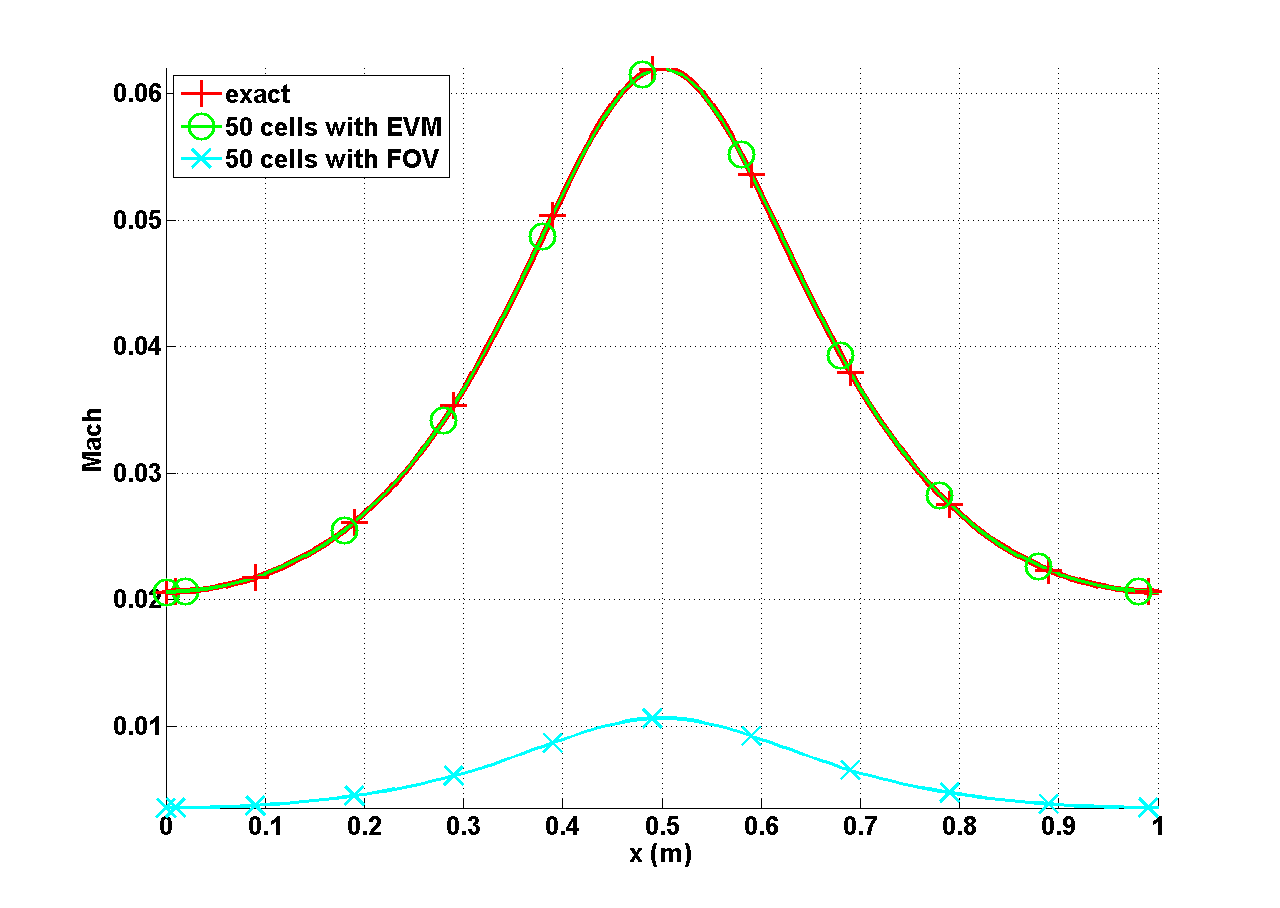
\includegraphics[width=\textwidth]{figures/liquid_mach_numerical_and_exact_50.png}
                \caption{Mach number}
                \label{fig:1d_nozzle_liq_vel}
        \end{subfigure}%

        \begin{subfigure}[b]{0.495\textwidth}
                \centering
                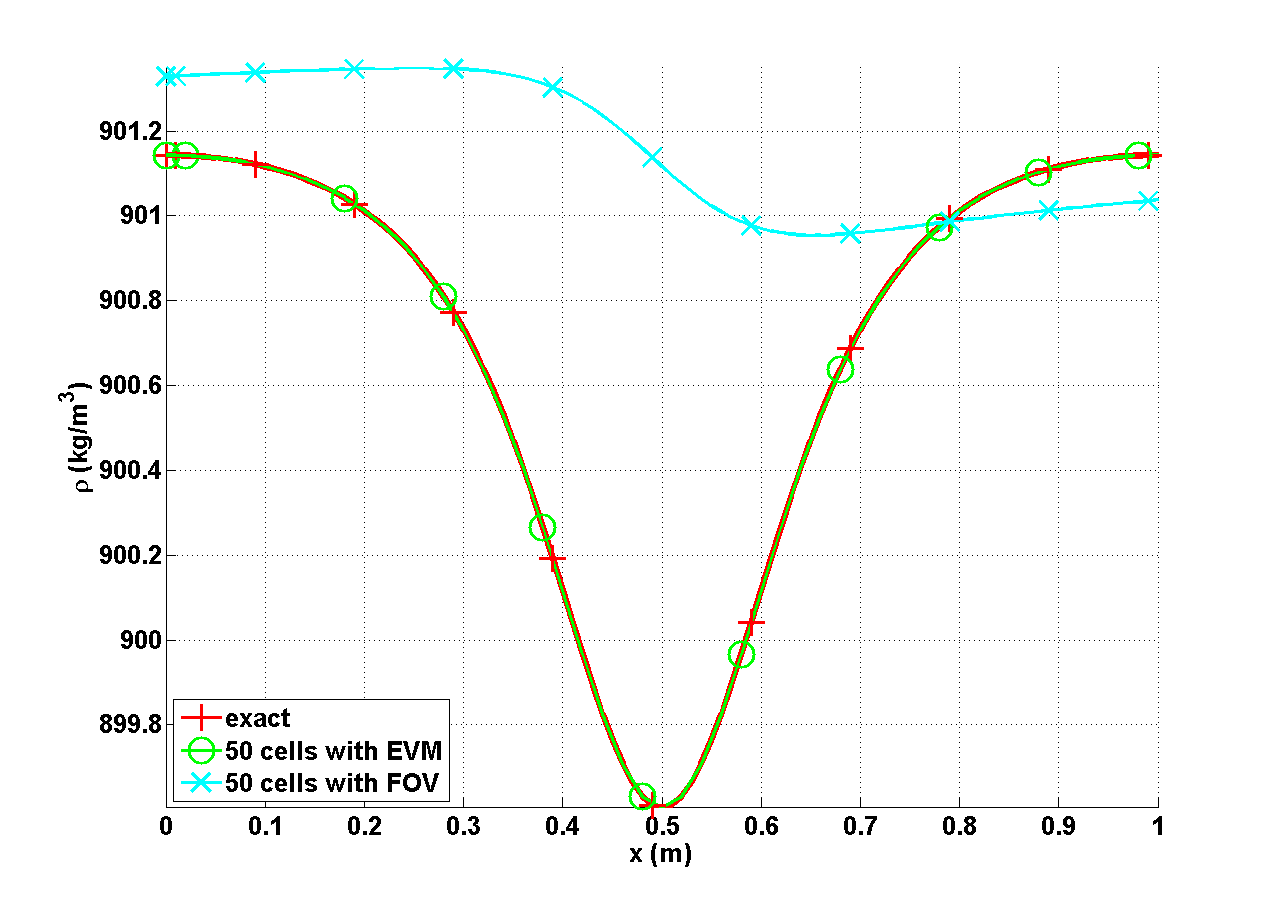
\includegraphics[width=\textwidth]{figures/liquid_density_numerical_and_exact_50.png}
                \caption{Density}
                \label{fig:1d_nozzle_liq_density}
        \end{subfigure}
        
        \begin{subfigure}[b]{0.495\textwidth}
                \centering
                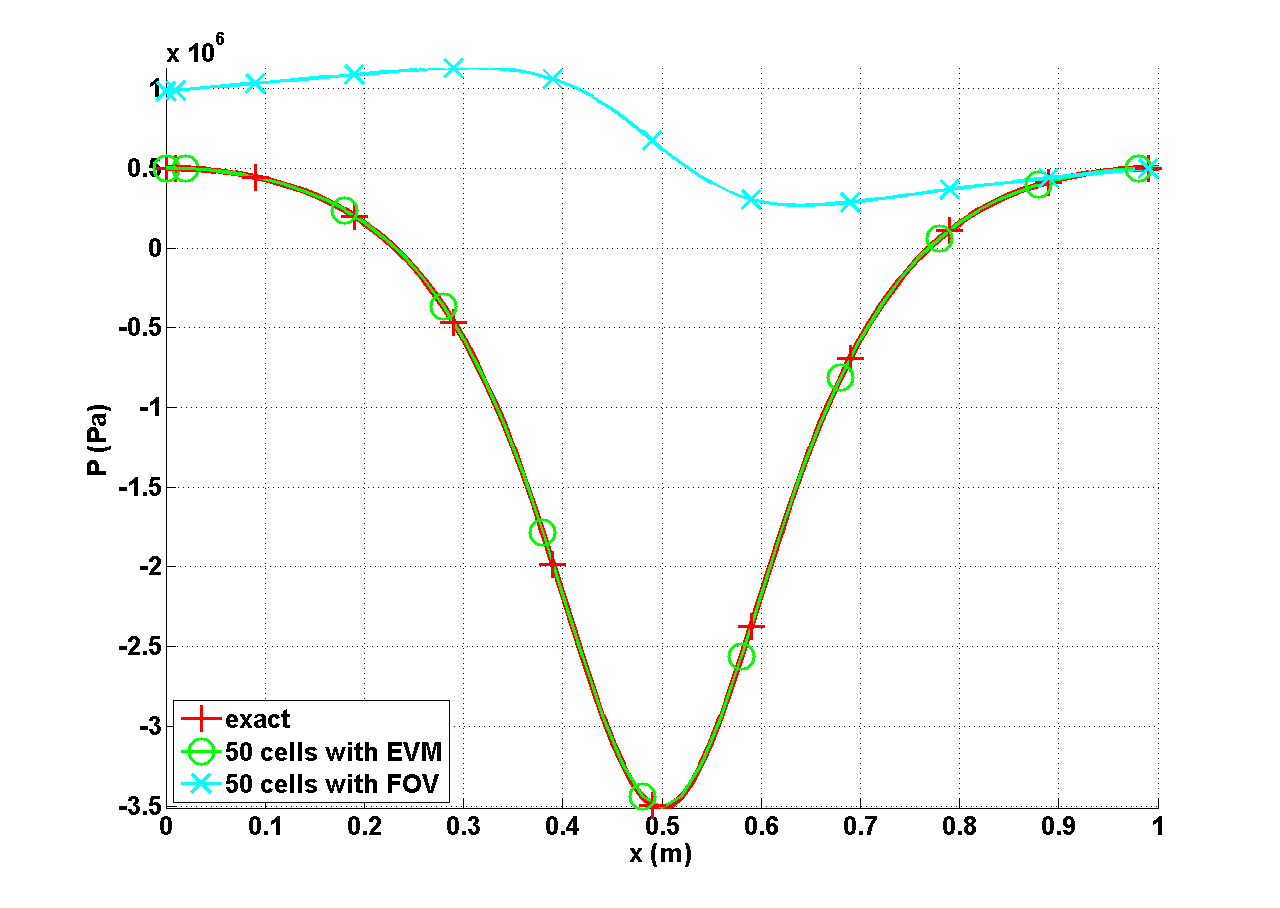
\includegraphics[width=\textwidth]{figures/liquid_pressure_numerical_and_exact_50.png}
                \caption{Pressure}
                \label{fig:1d_nozzle_liq_press}
        \end{subfigure}
        
        \begin{subfigure}[b]{0.495\textwidth}
                \centering
                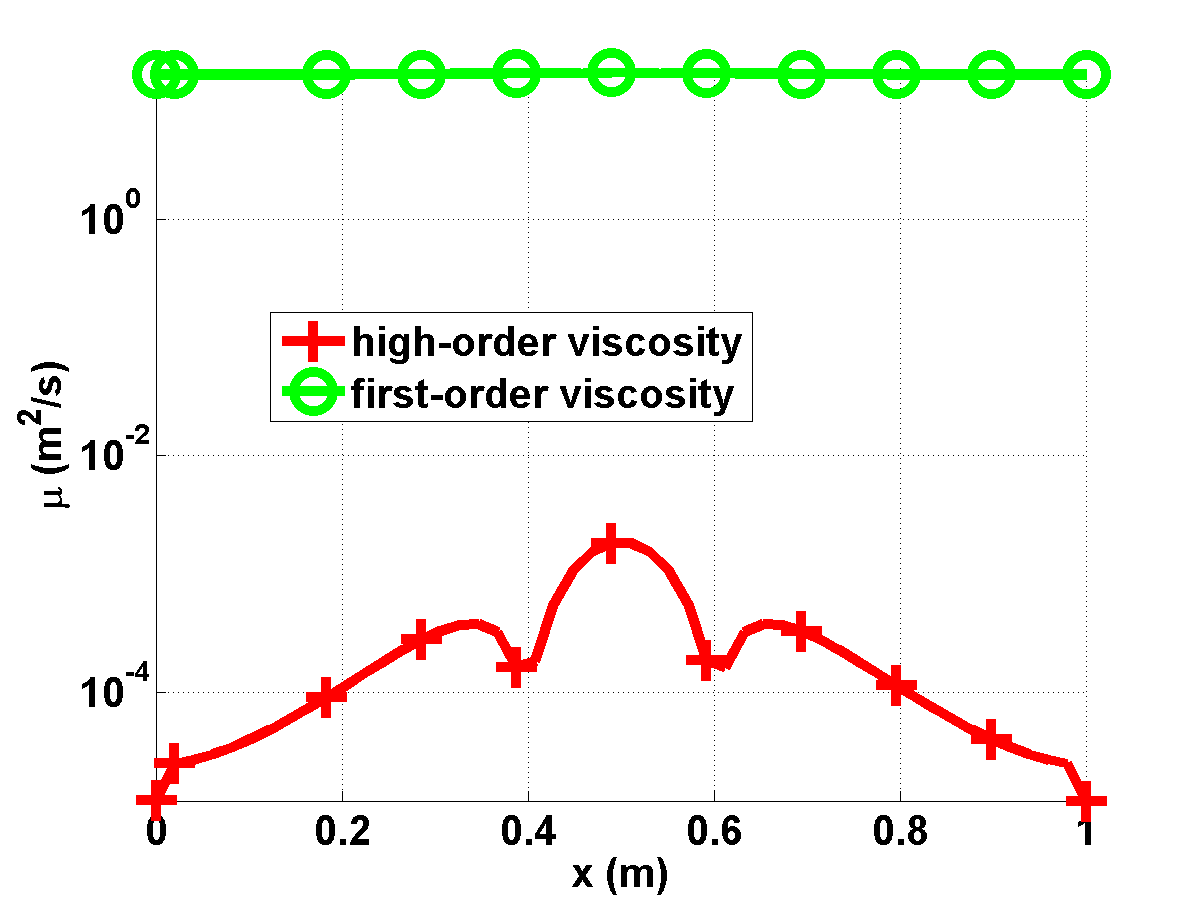
\includegraphics[width=\textwidth]{figures/liquid_viscosity_numerical50.png}
                \caption{Viscosity coefficients}
                \label{fig:1d_nozzle_liq_visc}
        \end{subfigure}
        \caption{Steady-state solution for a liquid flowing through a 1-D convergent-divergent nozzle.}\label{fig:1d_liq_nozzle}
\end{figure}
%
In \fig{fig:1d_liq_nozzle}, the numerical solutions obtained using the first-order viscosity (FOV) and the entropy viscosity method (EVM) are plotted against the exact solution. The numerical solution obtained with the EVM and the exact solution overlap, even for fairly coarse mesh (50 cells).
On the other hand, the numerical solution obtained with the FOV does not give the correct steady state: this is an illustration of the effect of ill-scaled dissipative terms. 
%
Note that the entropy viscosity coefficient is very small compared to the first-order one (\fig{fig:1d_nozzle_liq_visc}): (i) the numerical solution is smooth as shown in \fig{fig:1d_liq_nozzle} and (ii) the flow is in a low-Mach regime and thus isentropic . A convergence study was performed using the exact solution as a reference: the L$_1$ and L$_2$ norms of the error and the corresponding convergence rates are computed at steady state on various uniform mesh from 4 to 256 cells.
Spatial convergence results using linear finite elements are reported in \tbl{tbl:l1_norm_liq} and \tbl{tbl:l2_norm_liq} for the primitive variables: density, velocity and pressure.
%
\begin{table}[H]
\begin{center}
 \caption{\label{tbl:l1_norm_liq} L$_1$ norm of the error for the liquid phase in a 1-D convergent-divergent nozzle at steady state.}
 \begin{tabular}{|c|c|c|c|c|c|c|c|c|}
 \hline
cells & density         & rate   & pressure        & rate    & velocity         & rate     \\ \hline
4    & 2.8037 $10^{-1}$ & $-$    & 8.4705 $10^{5}$ & $-$     & 7.2737           & $-$      \\ \hline
8    & 1.3343 $10^{-1}$ & 0.495 & 4.7893 $10^{5}$ & 0.24 & 6.1493           & 0.0747 \\ \hline
16   & 2.9373 $10^{-2}$ & 2.10 & 1.0613 $10^{5}$ & 2.09  & 1.2275           & 2.25   \\ \hline
32   & 5.1120 $10^{-3}$ & 2.58 & 1.8446 $10^{4}$ & 2.58  & 1.8943 $10^{-1}$ & 2.78   \\ \hline
64   & 1.0558 $10^{-3}$ & 2.31 & 3.7938 $10^{3}$ & 2.31  & 3.7919 $10^{-2}$ & 2.37   \\ \hline
128  & 2.3712 $10^{-4}$ & 2.18 & 8.4471 $10^{2}$ & 2.19  & 8.5517 $10^{-3}$ & 2.17   \\ \hline
256  & 5.6058 $10^{-5}$ & 2.08 & 1.9839 $10^{2}$ & 2.09  & 2.0475 $10^{-3}$ & 2.07   \\ \hline
512  & 1.3278 $10^{-5}$ & $2.07$ & 4.6622 $10^{1}$ & 2.08  & 4.9516 $10^{-4}$ & $2.06$   \\ \hline
1024  & 3.1193 $10^{-6}$ & $-$ & 1.1755 $10^{1}$ & $-$  & 1.2379 $10^{-4}$ & $-$   \\ \hline
\end{tabular}
\end{center}
\end{table}
%
%
\begin{table}[H]
\begin{center}
 \caption{\label{tbl:l2_norm_liq} L$_2$ norm of the error for the liquid phase in a 1-D convergent-divergent nozzle at steady state.}
 \begin{tabular}{|c|c|c|c|c|c|c|c|c|}
 \hline
cells& density            & rate & pressure          & rate & velocity           & rate \\ \hline
4    & 3.106397 $10^{-1}$ & $-$  & 5.254445 $10^{5}$ & $-$  & 3.288543           & $-$  \\ \hline
8    & 7.491623 $10^{-2}$ & 2.06 & 1.636966 $10^{5}$ & 1.62 & 1.823880           & 0.14 \\ \hline
16   & 2.079858 $10^{-2}$ & 1.81 & 4.627338 $10^{4}$ & 1.77 & 4.990605 $10^{-1}$ & 1.83 \\ \hline
32   & 5.329627 $10^{-3}$ & 1.96 & 1.180287 $10^{4}$ & 1.96 & 1.261018 $10^{-1}$ & 1.98 \\ \hline
64   & 1.341583 $10^{-3}$ & 1.99 & 2.967104 $10^{3}$ & 1.99 & 3.160914 $10^{-2}$ & 1.99 \\ \hline
128  & 3.359766 $10^{-4}$ & 1.99 & 7.428087 $10^{2}$ & 1.99 & 7.907499 $10^{-3}$ & 1.99 \\ \hline
256  & 8.403859 $10^{-5}$ & 1.99 & 1.857861 $10^{2}$ & 2.01 & 1.977292 $10^{-3}$ & 2.00 \\ \hline
512  & 2.10075  $10^{-5}$ & $-$ & 4.7024   $10^{1}$ & $-$ & 4.9516   $10^{-4}$ & $-$ \\ \hline
\end{tabular}
\end{center}
\end{table}
% \tcr{check the rates in this table as well.} \tcb{I did and changed the values \\}
It is observed that the convergence rate for the L$_1$ and L$_2$ norm of the error is 2: the entropy viscosity method preserves the high-order accuracy when the numerical solution is smooth, and the new definition of the entropy viscosity coefficient behaves appropriately in the low-Mach limit.

%---------------------------------------------------------------------------------------------------
\subsection{Steam in a 1-D divergent-convergent nozzle} \label{sec:steam_nozzle}
%---------------------------------------------------------------------------------------------------

We use the same nozzle geometry, initial conditions and boundary conditions as in the previously example but replace liquid water with steam and use the steam parameters of the stiffened gas equation of state, \tbl{tbl:stff_gas_eos}. In this run, compressible effects will become dominant. 
The pressure difference between the inlet and outlet is large enough to accelerate the steam through the nozzle, leading to a formation of shock in the divergent portion of the nozzle. The behavior is different from what was observed for the liquid water phase in \sect{sec:liquid_nozzle} because of the liquid to gas density ratio is about $1,000$. An exact solution at steady state is available for the gas phase \cite{nozzle_exact}. The aim of this section is to show that when using the new definitions of the viscosity coefficients (\eqt{eq:final_def_visc_coeff}), the shock can be correctly resolved without spurious oscillations. The steady-state numerical solution, obtained using a uniform mesh with $1600$ cells, is shown in \fig{fig:1d_vap_nozzle}. The $CFL$ was set to $80$ (a high $CFL$ value can be used since the shock is stationary).

\begin{figure}[H]
        \centering
        \begin{subfigure}[b]{0.495\textwidth}
                \centering
                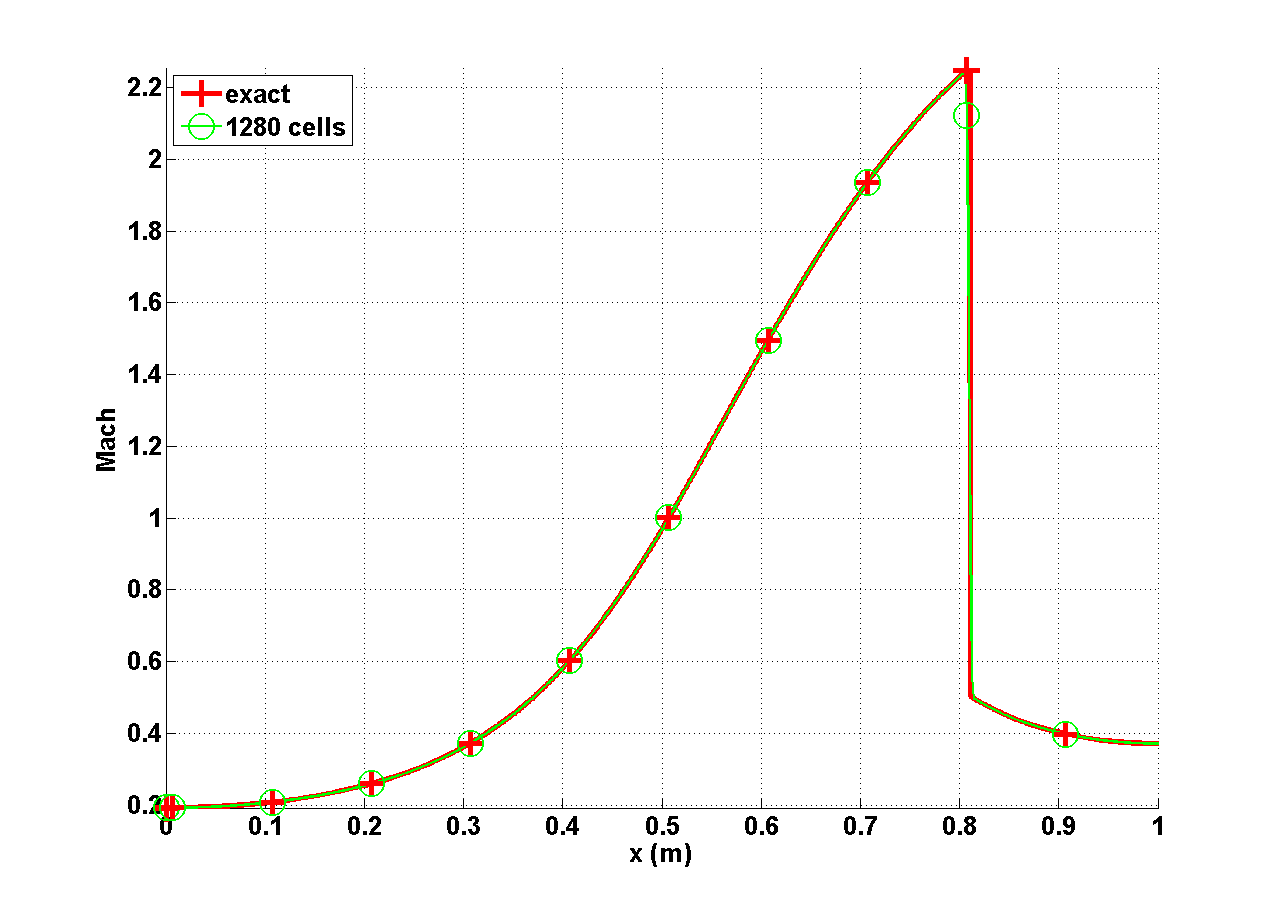
\includegraphics[width=\textwidth]{figures/vapor_mach_numerical_and_exact_1280.png}
                \caption{Mach number}
                \label{fig:1d_nozzle_vap_vel}
        \end{subfigure}%

        \begin{subfigure}[b]{0.495\textwidth}
                \centering
                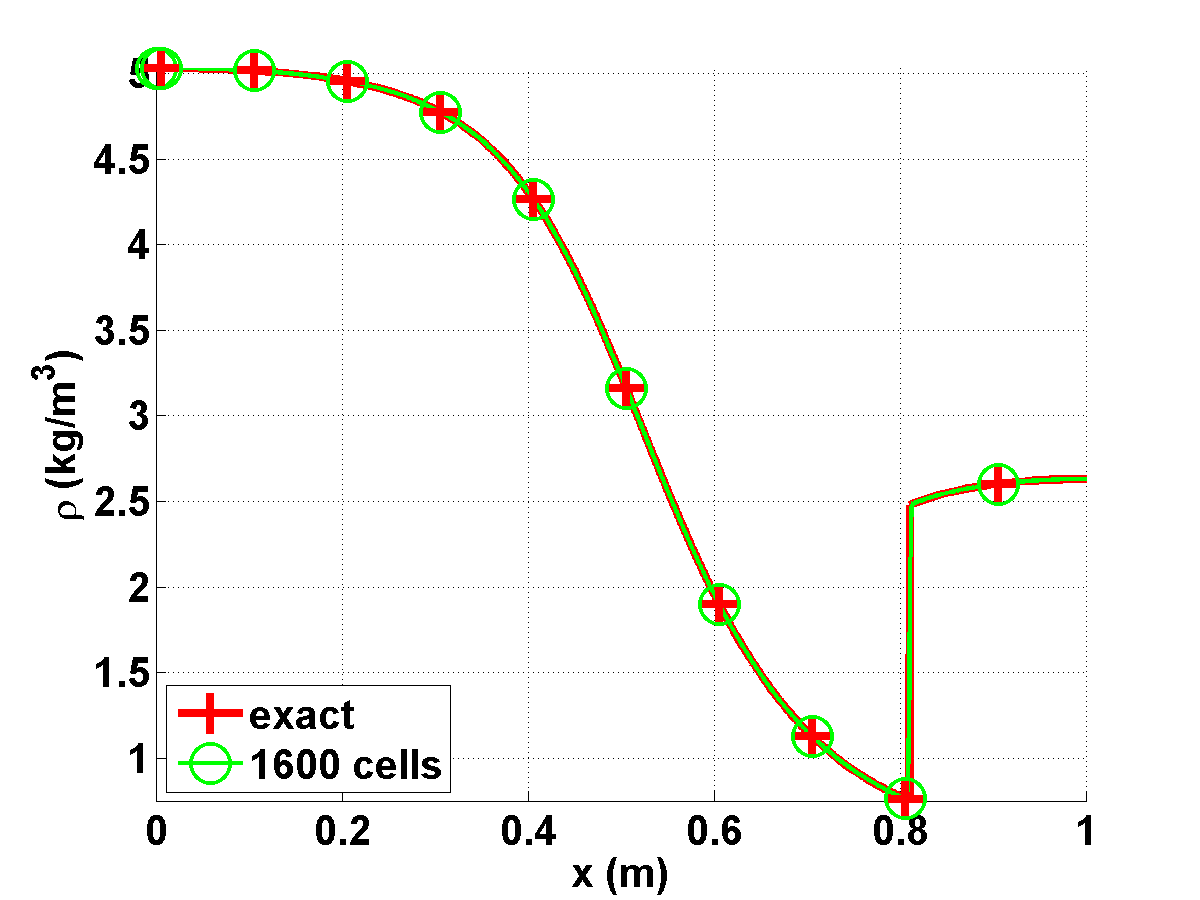
\includegraphics[width=\textwidth]{figures/vapor_density_numerical_and_exact_1600.png}
                \caption{Density}
                \label{fig:1d_nozzle_vap_density}
        \end{subfigure}

        \begin{subfigure}[b]{0.495\textwidth}
                \centering
                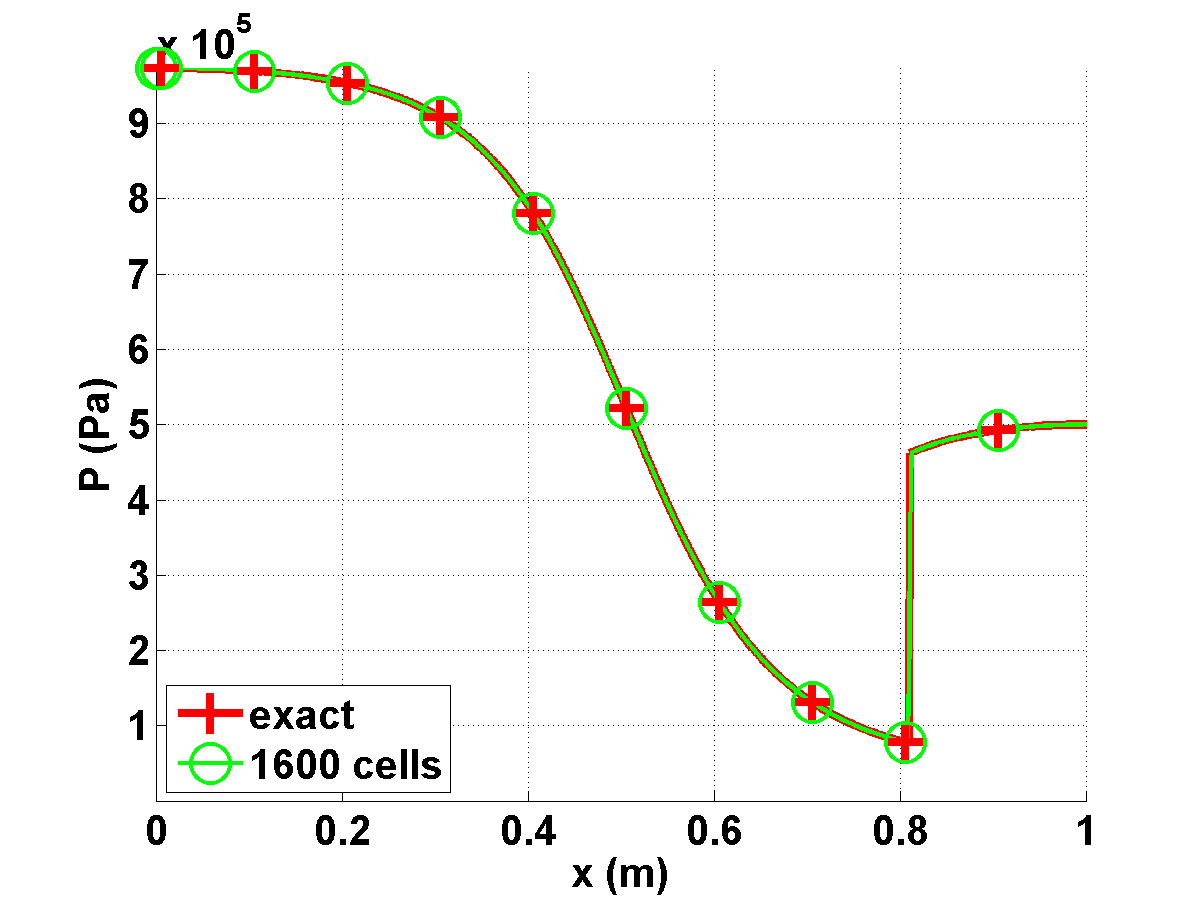
\includegraphics[width=\textwidth]{figures/vapor_pressure_numerical_and_exact_1600.png}
                \caption{Pressure}
                \label{fig:1d_nozzle_vap_press}
        \end{subfigure}

        \begin{subfigure}[b]{0.495\textwidth}
                \centering
                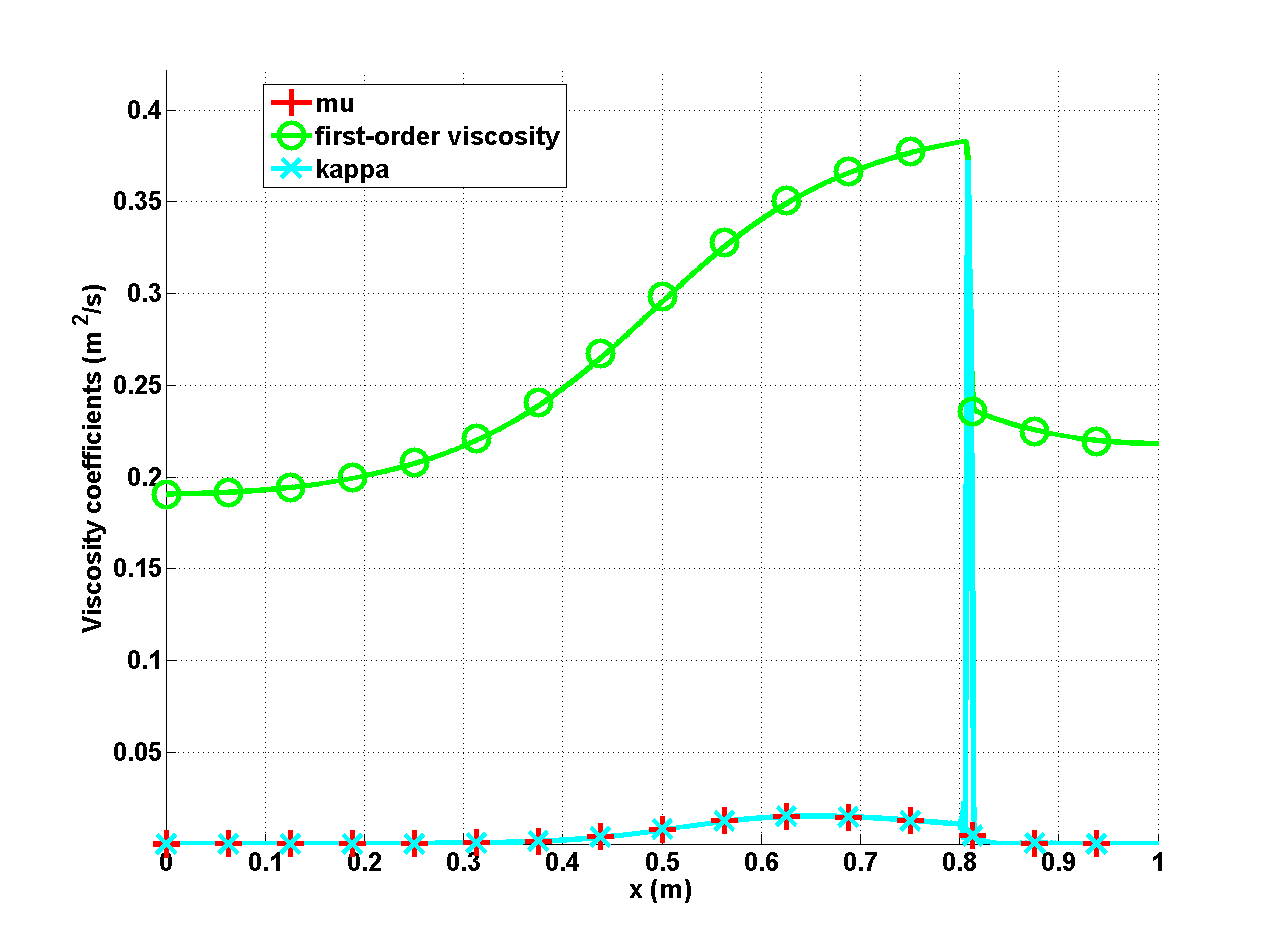
\includegraphics[width=\textwidth]{figures/vapor_viscosity_numerical1600.png}
                \caption{Viscosity coefficients}
                \label{fig:1d_nozzle_vap_visc}
        \end{subfigure}
        \caption{Steady-state solution for vapor phase flowing in a 1-D convergent-divergent nozzle.}
				\label{fig:1d_vap_nozzle}
\end{figure}
%
The steady-state solution of the density, Mach number and pressure are given in \fig{fig:1d_vap_nozzle}. The steady-solution exhibits a shock around $x=0.8m$ and matches the exact solution. In \fig{fig:1d_nozzle_vap_visc}, the first-order and entropy viscosity coefficients are plotted at steady-state (on a log scale): the entropy viscosity coefficient is peaked in the shock region around $x=0.8m$ as expected where it saturates to the first-order viscosity coefficient. The graph also presents another peak at $x=0.5m$  corresponding to the position of the sonic point for a 1-D convergent-divergent nozzle. This particular point is known to develop small instabilities that are detected when computing the jumps of the pressure and density gradients. Anywhere else, the entropy  viscosity coefficient is small. In order to prove convergence of the numerical solution to the exact solution, a convergence study is performed. Because of the presence of a shock, second-order accuracy is not expected and the convergence rate of a numerical solution should be 1 and $1/2$ when measured in the L$_1$ and L$_2$ norms, respectively (see Theorem 9.3 in \cite{convergence_book}). Results are reported in \tbl{tbl:l1_norm_vap} and \tbl{tbl:l2_norm_vap} for the primitive variables: density, velocity and pressure. The convergence rates for the L$_1$ and L$_2$ norms of the error computed using \eqt{eq:conv_rates} are in good agreement with the theoretical values.
%
\begin{table}[!htbp]
\begin{center}
 \caption{\label{tbl:l1_norm_vap} L$_1$ norm of the error for the vapor phase in a 1-D convergent-divergent nozzle at steady state.}
 \begin{tabular}{|c|c|c|c|c|c|c|c|c|}
 \hline
cells & density              & rate      & pressure          & rate      & velocity & rate      \\ \hline
$5$  & $0.72562$   $10^{-1}$ & $-$       & $1.5657$ $10^{5}$ & $-$       & $173.69$ & $-$       \\ \hline
$10$ & $0.4165$    $10^{-1}$ & $0.80088$ & $9.6741$ $10^{4}$ & $0.63425$ & $120.69$ & $0.52519$ \\ \hline
$20$ & $0.20675$   $10^{-1}$ & $1.0104$  & $4.9193$ $10^{4}$ & $0.96971$ & $72.149$ & $0.74228$ \\ \hline
$40$ & $0.093703$  $10^{-1}$ & $1.1417$  & $2.0103$ $10^{4}$ & $0.72728$ & $34.716$ & $1.0554$  \\ \hline
$80$ & $0.047328$  $10^{-1}$ & $0.9854$  & $1.0208$ $10^{4}$ & $0.9777$  & $16.082$ & $1.1101$  \\ \hline
$160$& $0.023965$  $10^{-2}$ & $0.9817$  & $5.1969$ $10^{3}$ & $0.9739$  & $7.9573$ & $1.0150$  \\ \hline
$320$& $0.020768$  $10^{-2}$ & $0.9886$  & $2.5116$ $10^{3}$ & $1.0490$  & $3.7812$ & $1.0734$  \\ \hline
$640$& $0.0059715$ $10^{-2}$ & $1.0160$  & $1.2754$ $10^{3}$ & $0.9776$  & $1.8353$ & $1.0428$  \\ \hline
\end{tabular}
\end{center}
\nonumber
\end{table}
\begin{table}[H]
\begin{center}
 \caption{\label{tbl:l2_norm_vap} L$_2$ norm of the error for the vapor phase in a 1-D convergent-divergent nozzle at steady state.}
 \begin{tabular}{|c|c|c|c|c|c|c|c|c|}
 \hline
cells & density             & rate      & pressure          & rate      & velocity & rate       \\ \hline
$5$   & $9.7144$ $10^{-1}$  & $-$       & $2.0215$ $10^{5}$ & $-$       & $236.94$ & $-$        \\ \hline
$10$  & $5.9718$ $10^{-1}$  & $0.70195$ & $1.3024$ $10^{5}$ & $0.63425$ & $166.56$ & $0.50854$  \\ \hline
$20$  & $2.9503$ $10^{-1}$  & $1.0173$  & $6.6503$ $10^{4}$ & $0.96971$ & $103.36$ & $0.68831$  \\ \hline
$40$  & $1.8193$ $10^{-1}$  & $0.69747$ & $4.0171$ $10^{4}$ & $0.72728$ & $66.374$ & $0.6390$   \\ \hline
$80$  & $1.3366$ $10^{-1}$  & $0.44485$ & $2.3163$ $10^{4}$ & $0.43576$ & $42.981$ & $0.62692$  \\ \hline
$160$ & $9.6638$ $10^{-2}$  & $0.46790$ & $1.7263$ $10^{4}$ & $0.42413$ & $31.717$ & $0.43844$  \\ \hline
$320$ & $7.0896$ $10^{-2}$  & $0.44688$ & $1.2763$ $10^{4}$ & $0.43571$ & $23.138$ & $0.45499$  \\ \hline
$640$ & $5.2191$ $10^{-2}$  & $0.44190$ & $9.4217$ $10^{3}$ & $0.43790$ & $16.910$ & $0.45238$  \\ \hline
\end{tabular}
\end{center}
\nonumber
\end{table}

%---------------------------------------------------------------------------------------------------
\subsection{Leblanc shock tube} \label{sec:Leblanc}
%---------------------------------------------------------------------------------------------------

The 1-D Leblanc shock tube is a Riemann problem designed to test the robustness and the accuracy of stabilization methods. The initial conditions are given in \tbl{tbl:ic_1d_tests}. The ideal gas equation of state (with $\gamma=5/3$) is used to compute the pressure.
This test is computationally challenging because of the large pressure ratio at the shock interface.
The computational domain consists of a 1-D straight pipe of length $L=9m$ with the initial interface located at $x=2m$. At $t=0.s$, the interface is removed. The numerical solution is run until $t=4 s$ and the density, momentum and total energy profiles are given in \fig{fig:1d_leblanc}, along with the exact solution. The viscosity coefficients are also plotted in \fig{fig:1d_leblanc_visc}. These plots were  run with three different uniform mesh of $800$, $3200$ and $6000$ cells and a constant $CFL = 1$.
\begin{figure}[H]
        \centering
        \begin{subfigure}[b]{0.495\textwidth}
                \centering
                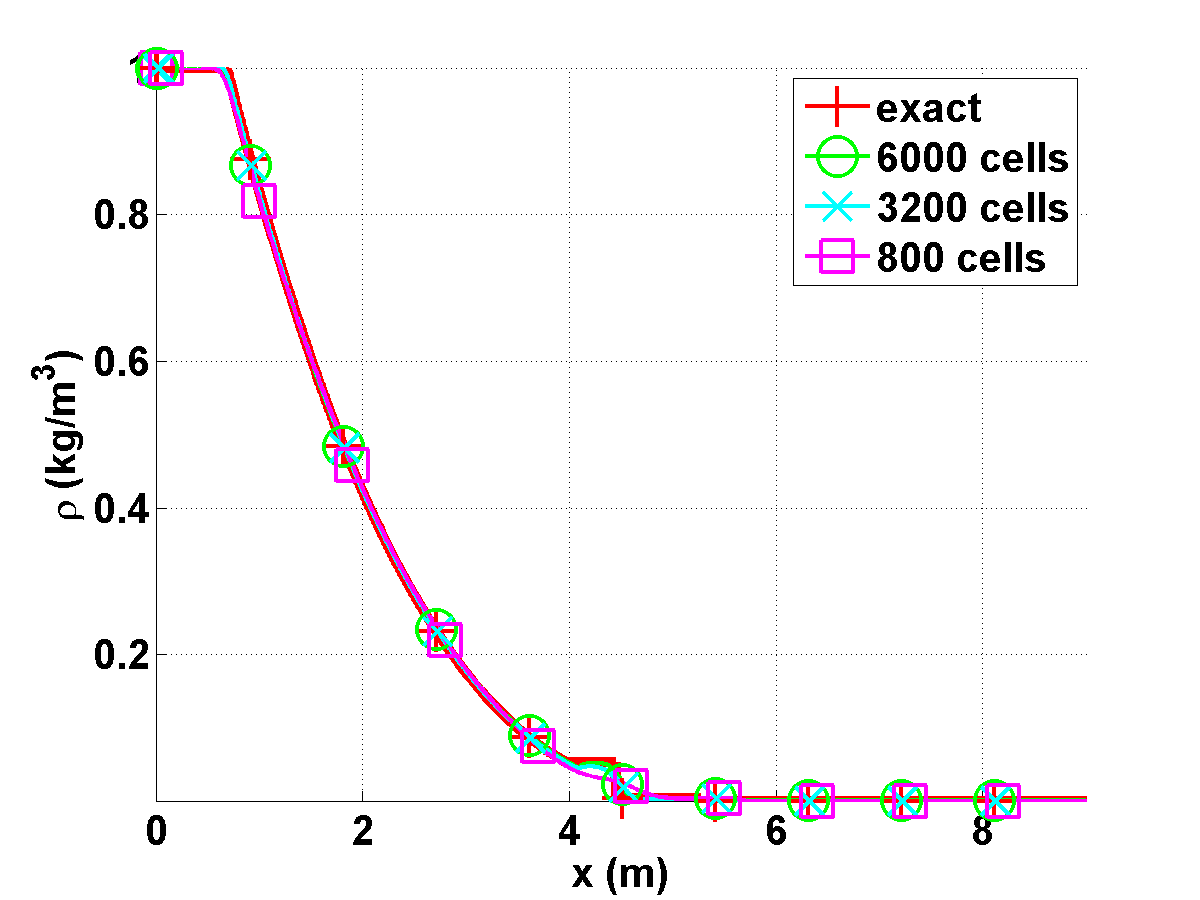
\includegraphics[width=\textwidth]{figures/Leblanc_exact_and_numerical_stt_density_6000.png}
                \caption{Density}
                \label{fig:1d_leblanc_vel}
        \end{subfigure}%
        %add desired spacing between images, e. g. ~, \quad, \qquad etc. 
          %(or a blank line to force the subfigure onto a new line)
        \begin{subfigure}[b]{0.495\textwidth}
                \centering
                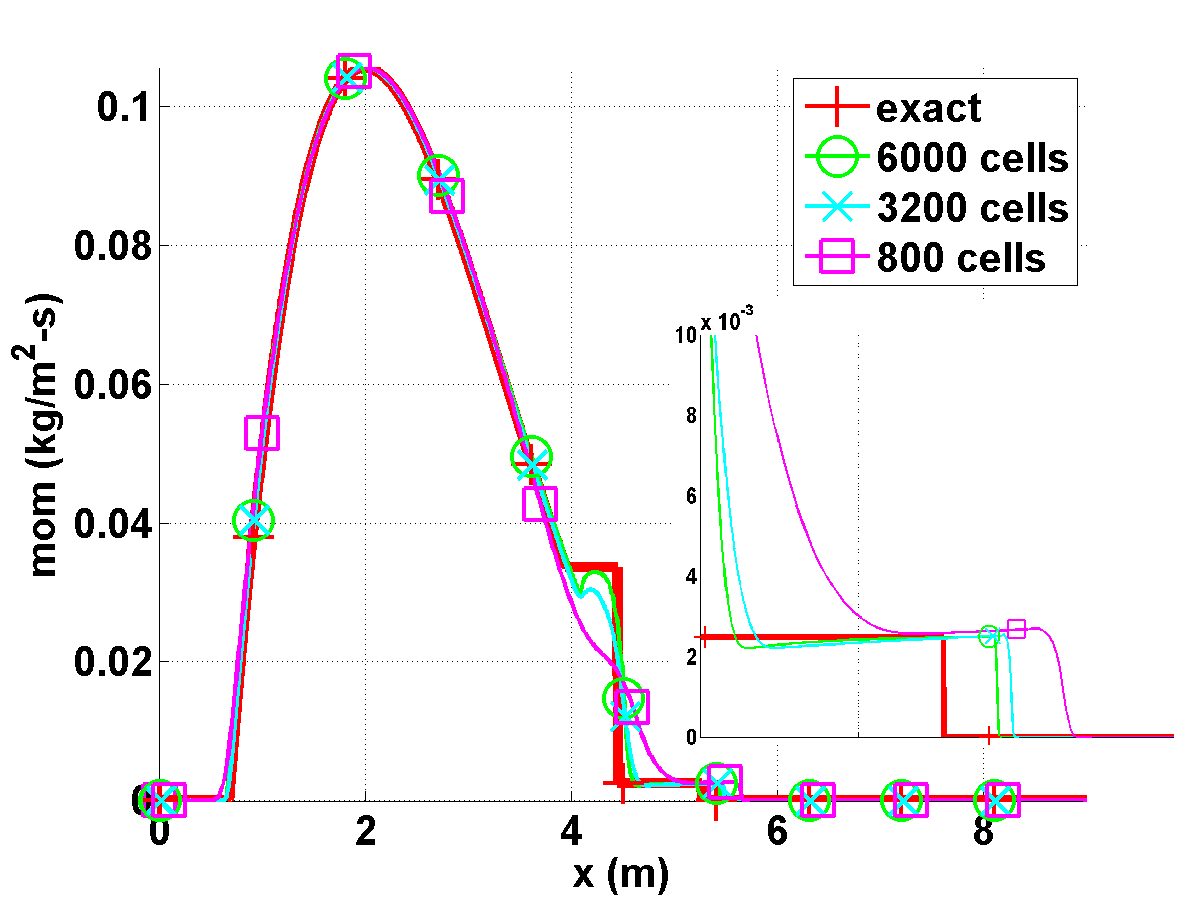
\includegraphics[width=\textwidth]{figures/Leblanc_exact_and_numerical_stt_momentum_6000.png}
                \caption{Momentum}
                \label{fig:1d_leblanc_density}
        \end{subfigure}
         %add desired spacing between images, e. g. ~, \quad, \qquad etc. 
          %(or a blank line to force the subfigure onto a new line)
        \begin{subfigure}[b]{0.495\textwidth}
                \centering
                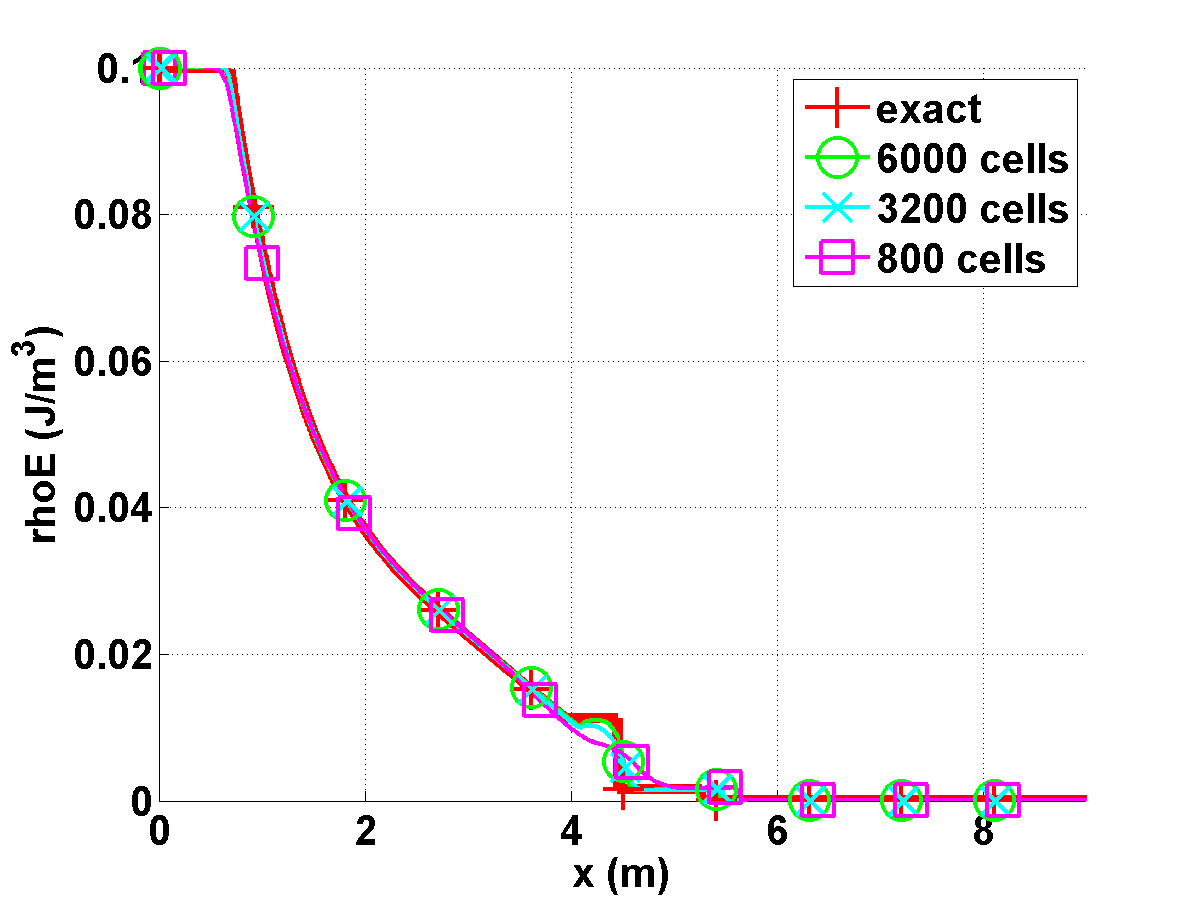
\includegraphics[width=\textwidth]{figures/Leblanc_exact_and_numerical_stt_total_energy_6000.png}
                \caption{Total energy}
                \label{fig:1d_leblanc_press}
        \end{subfigure}
          %add desired spacing between images, e. g. ~, \quad, \qquad etc. 
          %(or a blank line to force the subfigure onto a new line)
        \begin{subfigure}[b]{0.495\textwidth}
                \centering
                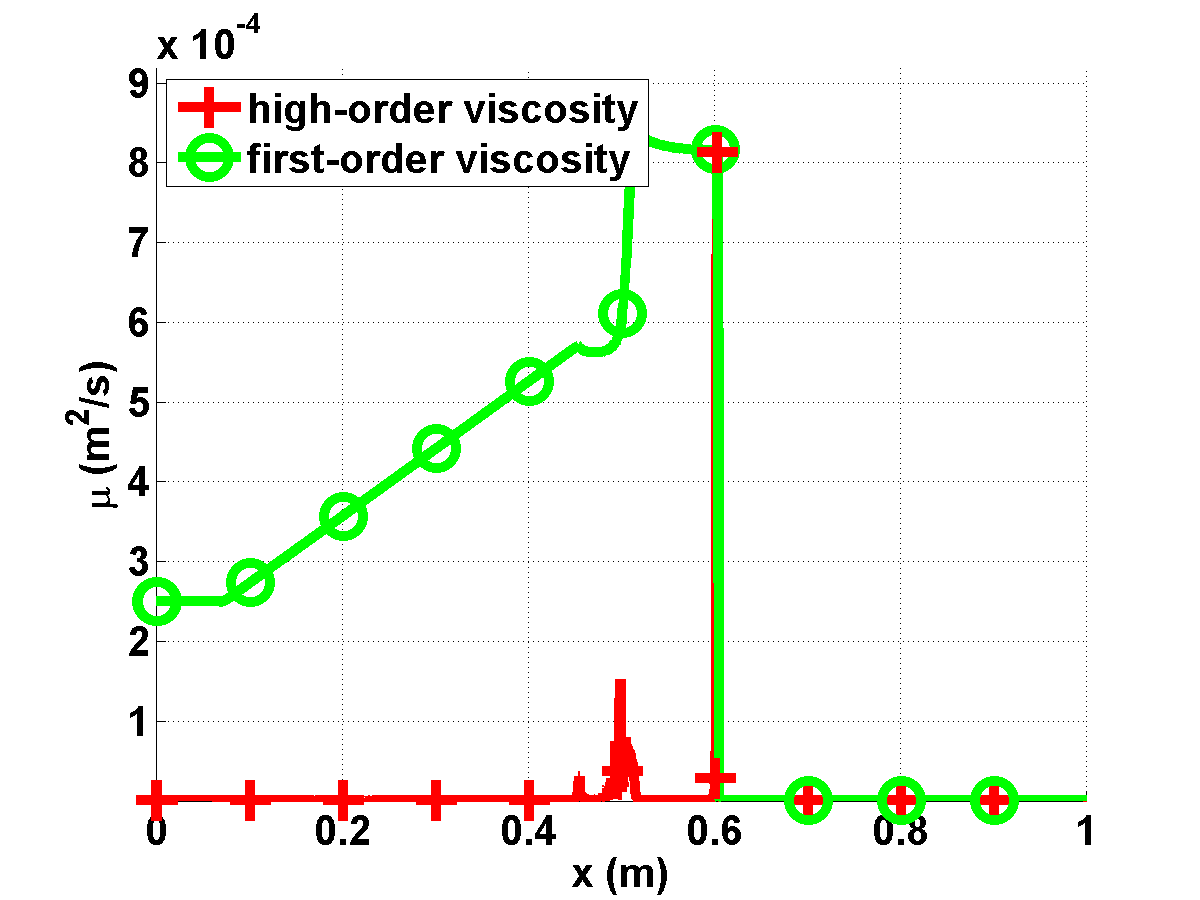
\includegraphics[width=\textwidth]{figures/Leblanc_viscosity_numerical_6000.png}
                \caption{Viscosity coefficients}
                \label{fig:1d_leblanc_visc}
        \end{subfigure}
        \caption{Exact and Numerical solutions for the 1-D Leblanc shock tube at $t=4 s$.}\label{fig:1d_leblanc}
\end{figure}
%
The density, momentum and total energy profiles are provided in \fig{fig:1d_leblanc}. In \fig{fig:1d_leblanc_density}, the shock region is zoomed in for better resolution: the shock is well resolved. We also observe that the shock position computed numerically converges to the exact position under mesh refinement. The contact wave at $x=4.5m$ can be seen in \fig{fig:1d_leblanc_density}. The entropy viscosity coefficient profile is shown in \fig{fig:1d_leblanc_visc} and behaves as expected: it saturates to the first-order viscosity in the shock region, thus preventing oscillations from forming. At the location of the contact wave, a smaller peak is observed that is due to the presence of the jumps in the definition of the entropy viscosity coefficient (\eqt{eq:final_def_visc_coeff}).  The Mach number, not plotted, is of the order of $1.3$ right before the shock and reaches a maximum value close to $5$ in the contact region.

Once again, a convergence study is performed in order to prove convergence of the numerical solution to the exact solution. As in the previous example (vapor phase in the 1-D nozzle, \sect{sec:steam_nozzle}), the expected convergence rates in the L$_1$ and L$_2$ norms are 1 and $1/2$, respectively. The exact solution was obtained by running a 1-D Riemann solver and used as the reference solution to compute the L$_1$ and L$_2$-norms that are reported in \tbl{tbl:l1_norm_leblanc} and \tbl{tbl:l2_norm_leblanc} for the conservative variables: density, momentum and total energy. The convergence rates are again approaching the theoretical values.

\begin{table}[!htbp]
\begin{center}
 \caption{\label{tbl:l1_norm_leblanc} L$_1$ norm of the error for the 1-D Leblanc test at $t=4s$.}
 \begin{tabular}{|c|c|c|c|c|c|c|c|c|}
 \hline
  cells & density               & rate         & momentum              & rate          & total energy          & rate         \\  \hline
$100$   & $1.0354722$ $10^{-2}$ & $-$          & $3.5471714$ $10^{-3}$ & $-$           & $1.4033046$ $10^{-3}$ & $-$          \\  \hline
$200$   & $7.2680512$ $10^{-3}$ & $0.51064841$ & $2.5933119$ $10^{-3}$ & $0.45187331$  & $9.8611746$ $10^{-4}$ & $0.5089968$  \\  \hline
$400$   & $5.0825628$ $10^{-3}$ & $0.51601245$ & $2.0668092$ $10^{-3}$ & $0.32739054$  & $7.7844421$ $10^{-4}$ & $0.34116585$ \\  \hline
$800$   & $3.4025056$ $10^{-3}$ & $0.57895861$ & $1.4793838$ $10^{-3}$ & $0.48240884$  & $5.5702549$ $10^{-4}$ & $0.48285029$ \\  \hline
$1600$  & $2.1649953$ $10^{-3}$ & $0.65223363$ & $9.7152832$ $10^{-4}$ & $0.6066684$   & $3.5720171$ $10^{-4}$ & $0.64100438$ \\  \hline
$3200$  & $1.2465433$ $10^{-3}$ & $0.79643094$ & $5.5937409$ $10^{-4}$ & $0.79644263$  & $2.0491799$ $10^{-4}$ & $0.80169235$ \\  \hline
$6400$  & $6.4476928$ $10^{-4}$ & $0.95107804$ & $3.0244198$ $10^{-4}$ & $0.88715502$  & $1.0914891$ $10^{-4}$ & $0.90874889$ \\  \hline
$12800$ & $3.3950948$ $10^{-4}$ & $0.92533116$ & $1.5958118$ $10^{-4}$ & $0.9223679$   & $5.7909794$ $10^{-5}$ & $0.91441847$ \\  \hline
 \end{tabular}
\end{center}
\end{table}
%
\begin{table}[!htbp]
\begin{center}
 \caption{\label{tbl:l2_norm_leblanc} L$_2$ norm of the error for the 1-D Leblanc test at $t=4s$.}
 \begin{tabular}{|c|c|c|c|c|c|c|}
 \hline
   cells & density & rate & momentum & rate & total energy & rate \\ \hline
$100$ &   $5.7187851$ $10^{-3}$ & $-$ & $1.7767236$ $10^{-3}$ & $-$ & $7.6112265$  $10^{-4}$& $-$\\   \hline
$200$  &  $3.8995238$ $10^{-3}$ & $0.55241073$ & $1.4913161$ $10^{-3}$ & $0.25263314$ &  $5.5497308$ $10^{-4}$& $0.45571115$\\ \hline
$400$ & $2.8103526$ $10^{-3}$   & $0.4725468$ & $1.3305301$ $10^{-3}$ & $0.164585$ & $4.6063172$ $10^{-4}$ & $0.26880405$\\ \hline
$800$ & $2.1081933$ $10^{-3}$   & $0.41474398$ & $1.1398931$ $10^{-3}$ & $0.22310254$ & $3.7798953$ $10^{-4}$ & $0.28526749$\\ \hline
$1600$ & $1.5731052$ $10^{-3}$  & $0.42239201$ & $9.0394227$ $10^{-4}$ & $0.33459602$ & $2.9584646$ $10^{-4}$ & $0.35349763$\\ \hline
$3200$&$1.0610667$ $10^{-3}$    & $0.56809979$ & $6.2735595$ $10^{-4}$ & $0.52694639$ & $2.054455$ $10^{-4}$ & $0.52609289$\\ \hline
$6400$&$7.3309974$ $10^{-4}$    & $0.53343397$ & $4.4545754$ $10^{-4}$ & $0.49399631$ & $1.4670834$ $10^{-4}$ & $0.48580482$\\ \hline
 $12800$&$5.1020991$ $10^{-4}$  & $0.52291857$ & $3.1266758$ $10^{-4}$ & $0.5106583$ & $1.0299897$ $10^{-5}$ & $0.51032105$\\  \hline
\end{tabular}
\end{center}
\nonumber
\end{table}

%---------------------------------------------------------------------------------------------------
\subsection{1-D shock tube with a liquid phase} \label{sec:liquid_shock}
%---------------------------------------------------------------------------------------------------
%\tcr{until now, you never gave the mu and kappa coefficients, yet they are now different due to their different normalizations.
%Maybe very little for the previous cases, but we need to mention something because, in this section, you show both, and it is better
%to say something than to let the reviewers wonder ... } \tcb{what do you think of the following?}
The purpose of this test is to investigate the ability of the entropy viscosity method to stabilize a strong shock with a small Mach number \cite{abgrall}: the Mach number in the shock region is of the order of 0.1. In this case, as explained in \sect{sec:lowMach}, the viscosity coefficients are required to have different order of magnitude in order to ensure the correct scaling of the dissipative terms. This test will allows us to validate the approach presented in \sect{sec:lowMach}.  

The stiffened gas equation of state is used to model a liquid flow with the parameters given in \tbl{tbl:stff_gas_eos}. The computational domain of length $L=1m$ is uniformly discretized using 500 cells. The step initial conditions are given in \tbl{tbl:ic_1d_tests}.
%
The simulation is run with a $CFL=1$ until the final time $t_{\text{final}} = 7 \ 10^{-5}s$. Results for pressure, density, velocity and the viscosity coefficients are given in \fig{fig:1d_strong_shock} along with the exact solution for comparison purposes. The numerical solution is in good agreement with exact solution in \fig{fig:1d_strong_shock_var}. The viscosity coefficients $\mu$ and $\kappa$ are not equal in the shock because the Mach number is of order $0.1$. The viscosity coefficient $\kappa$ saturates to the first-order viscosity in the shock region around $x = 0.65m$ and is sufficient to stabilize the numerical scheme. 
%This example illustrates the capabilities of the entropy viscosity method to stabilize a strong shock using liquid fluid properties. 
%
\begin{figure}[H]
        \centering
        \begin{subfigure}[b]{0.495\textwidth}
                \centering
                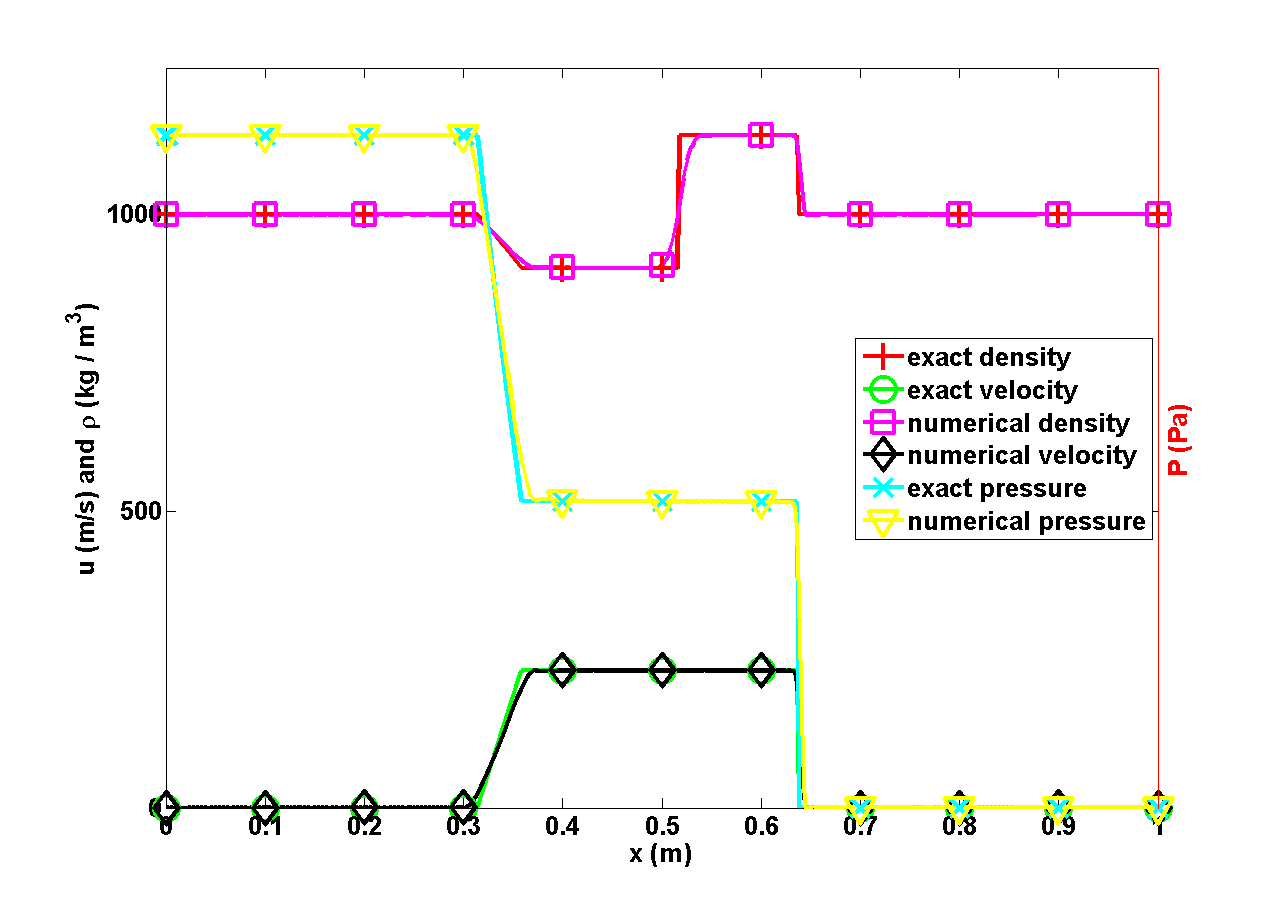
\includegraphics[width=\textwidth]{figures/LiquidSrongShock_density_velocity_pressure_profiles.png}
                \caption{Density, velocity and pressure profiles.}
                \label{fig:1d_strong_shock_var}
        \end{subfigure}%

        \begin{subfigure}[b]{0.495\textwidth}
                \centering
                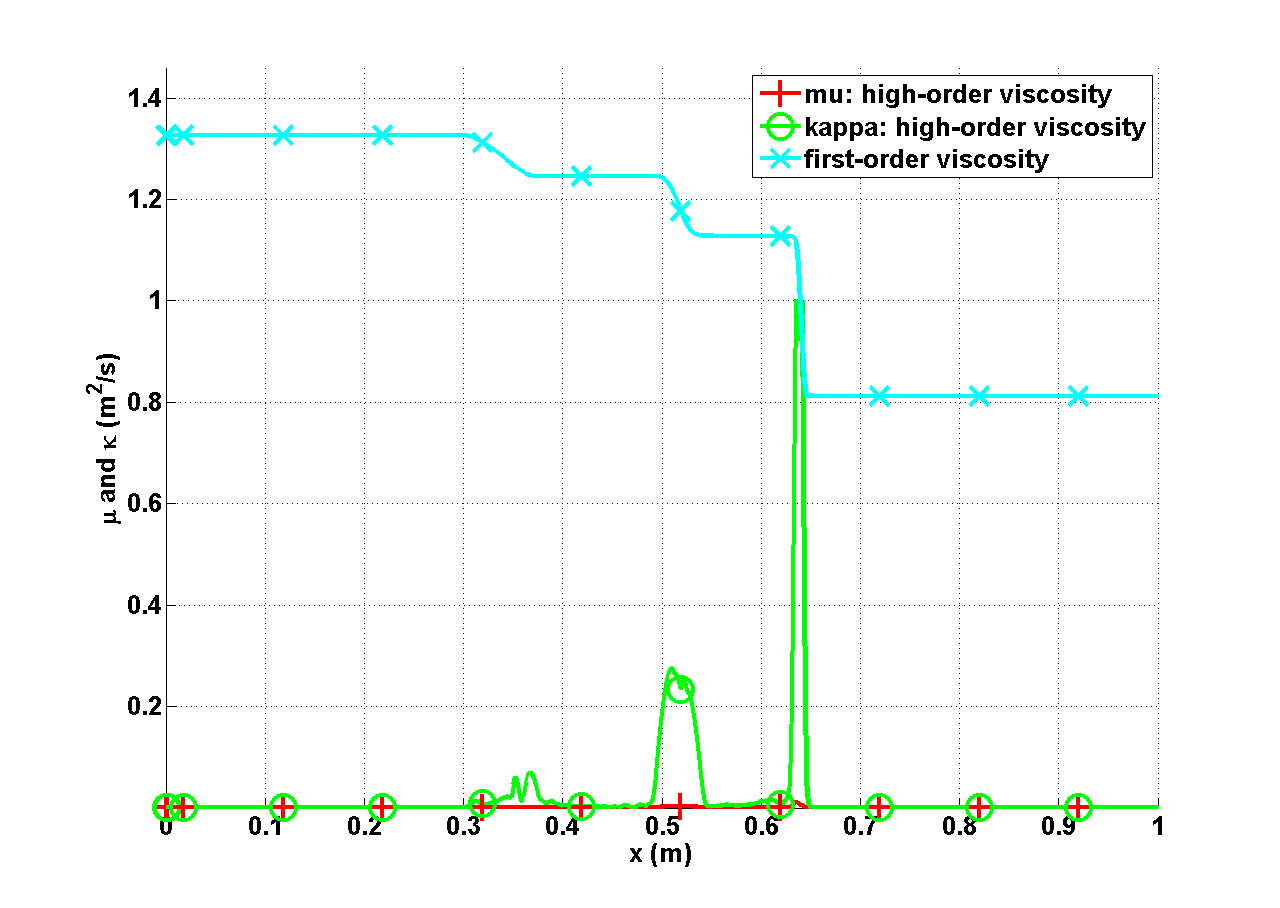
\includegraphics[width=\textwidth]{figures/LiquidSrongShock_viscosity.png}
                \caption{Viscosity coefficients profile.}
                \label{fig:1d_strong_shock_visc}
        \end{subfigure}
        \caption{Numerical solution for the 1-D liquid shock tube at  at $t_{\text{final}} = 7 \  10^{-5}s$.}
				\label{fig:1d_strong_shock}
\end{figure}


%---------------------------------------------------------------------------------------------------
\subsection{1-D slow moving shock} \label{sec:slow_moving_shock}
%---------------------------------------------------------------------------------------------------

Slow moving shocks are known to produce post-shock noise of low frequency that are not damped by some numerical dissipation methods \cite{james}. The aim of this simulation is to test the ability of the entropy viscosity method to dampen the low frequency waves.
The 1-D slow moving shock consists of a shock wave moving from left to right with the initial conditions given in \tbl{tbl:ic_1d_tests}. The ideal gas equation of state is used with a heat capacity ratio $\gamma=1.4$.  In order to make the shock travel a significant distance, the final time is taken equal to $t=1.1s$. A pressure boundary condition is used at the left boundary to let the rarefaction and contact waves exit the domain.   
%
The numerical solution, obtained with 200 equally-spaced cells, is given in \fig{fig:low_moving_shock} and is compared to the exact solution obtained from a Riemann solver. We use a $CFL$ of 1. With this $CFL$ value, it takes about 50 time steps for the shock to traverse one cell.
%
The numerical results are in good agreement with the exact solution and do not display any post-shock noise. The rarefaction and contact waves are not visible on \fig{fig:profiles_sms} since they exited the computational domain through the left pressure boundary condition earlier. As explained in \cite{roberts}, Godunov's type method usually fails to resolve a slow moving shock because of the nature of the stabilization method: the method scales as the eigenvalue of the appropriate field. In the case of a slow moving shock, the dissipation added to the system is under-estimated and leads to post-shock noise. In the case of the entropy viscosity method, the entropy residual detects the shock position and the viscosity coefficients saturate to the first-order viscosity values in the shock region. The main difference between a  Godunov's type method and the entropy viscosity method relies in the definition of the first-order viscosity coefficients that are proportional to the \emph{local maximum eigenvalue} $||\vec{u}||+c$ and not to the eigenvalue of the characteristic field.
%
\begin{figure}[H]
        \centering
        \begin{subfigure}[b]{0.495\textwidth}
                \centering
                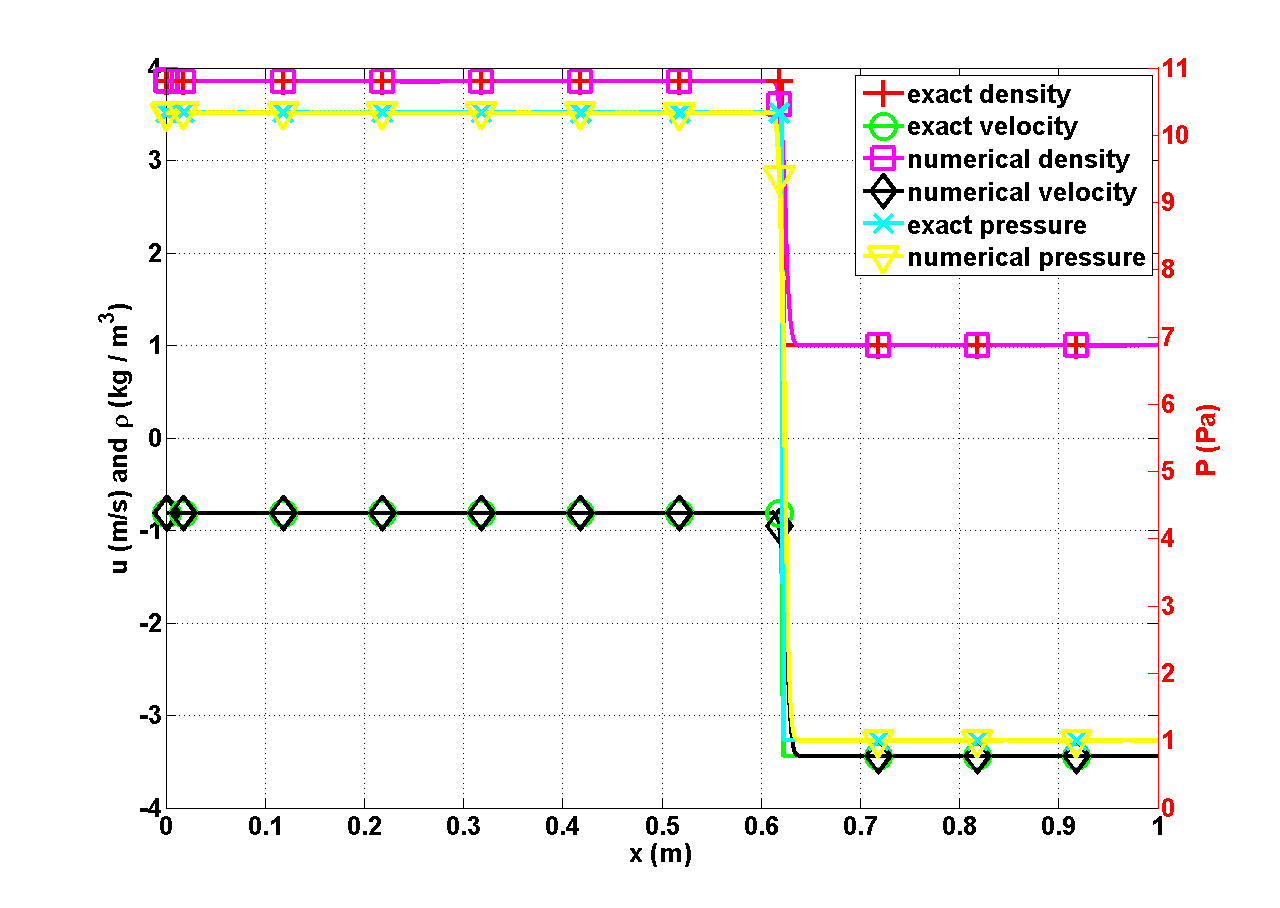
\includegraphics[width=\textwidth]{figures/SlowMovingShock_density_velocity_pressure_profiles.png}
                \caption{Velocity, density and pressure}
                \label{fig:profiles_sms}
        \end{subfigure}%

        \begin{subfigure}[b]{0.495\textwidth}
                \centering
                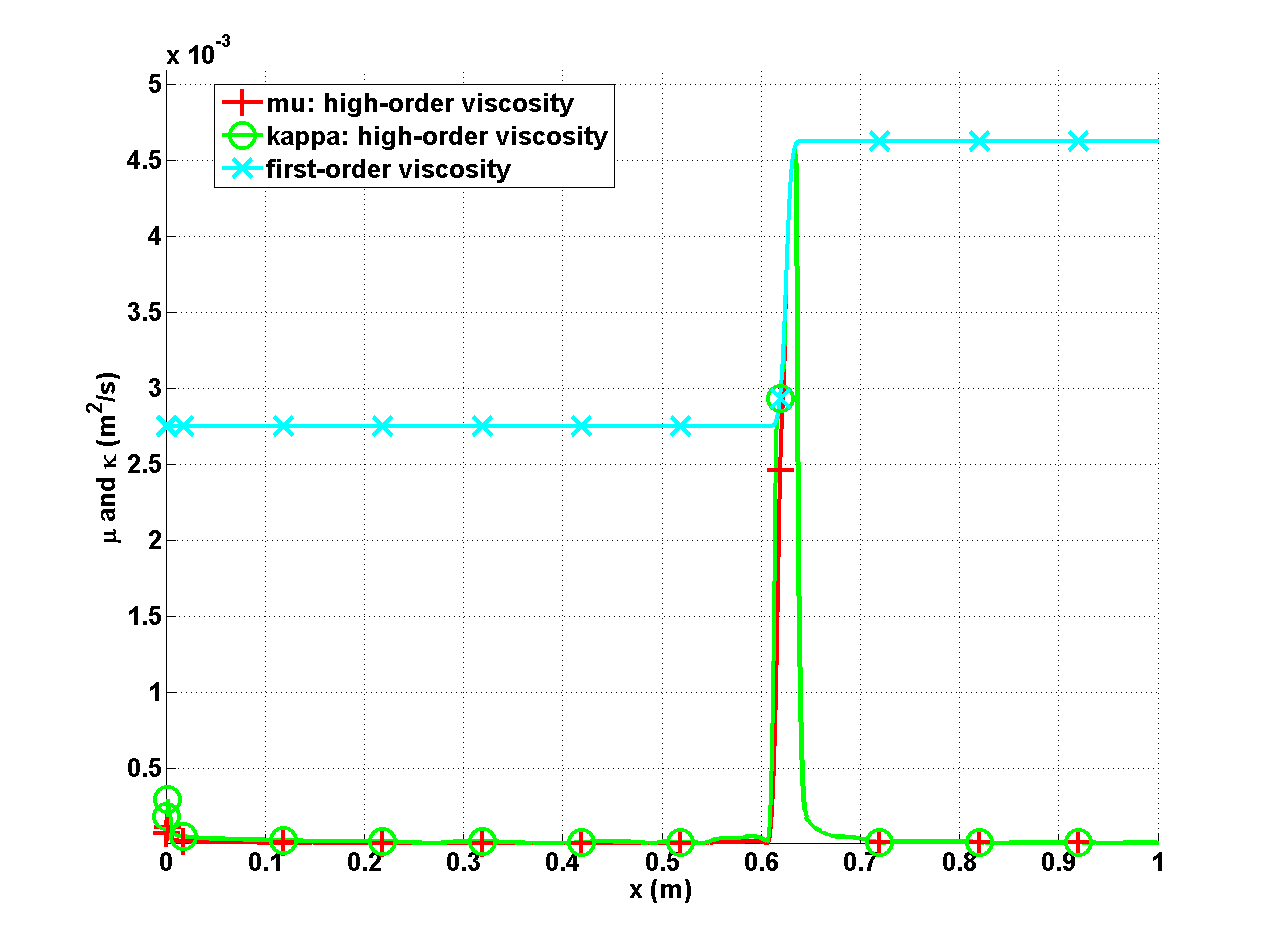
\includegraphics[width=\textwidth]{figures/SlowMovingShock_viscosity.png}
                \caption{Viscosity coefficients}
                \label{fig:viscosity_sms}
        \end{subfigure} 
        \caption{Slow moving shock profiles at $t=1.1s$.}\label{fig:low_moving_shock}
\end{figure} 

%---------------------------------------------------------------------------------------------------
\subsection{Typical $1$-D shock tubes \cite{Toro}} \label{sec:1d_toro}
%---------------------------------------------------------------------------------------------------
%%%%%%%%%%%%%%%%%%%%%%%%%%%%%%%%%%%%%%%%%%%%%%%%%%%%%%%%%%%%%%%%%%%%%%%%%%%%%%%%%%%%%%%%%%%%%%%%%%%%
%%%%%%%%%%%%%%%%%%%%%%%%%%%%%%%%%%%%%%%%%%%%%%%%%%%%%%%%%%%%%%%%%%%%%%%%%%%%%%%%%%%%%%%%%%%%%%%%%%%%
\section{$2$-D numerical results for supersonic flows:} \label{sec:2d-supersonic-results}
%%%%%%%%%%%%%%%%%%%%%%%%%%%%%%%%%%%%%%%%%%%%%%%%%%%%%%%%%%%%%%%%%%%%%%%%%%%%%%%%%%%%%%%%%%%%%%%%%%%%
%%%%%%%%%%%%%%%%%%%%%%%%%%%%%%%%%%%%%%%%%%%%%%%%%%%%%%%%%%%%%%%%%%%%%%%%%%%%%%%%%%%%%%%%%%%%%%%%%%%%
This section focuses on demonstrating the ability of the entropy viscosity method, with the new definition of the viscosity coefficients derived in \sect{sec:lowMach}, to accurately resolve shocks occurring in transonic flows. Such tests were already performed in \cite{valentin} with the former definition of the entropy viscosity method recalled in \sect{sec:background}, and using a discontinuous Galerkin finite element discretization. Our objective here, is to show that the new definition of the viscosity coefficients is still capable of resolving shocks. The numerical tests presented in this section include: flow pass a forward facing step (REFS), a circular explosion (REFS), a steady-state flow over a double wedge and a steady-state flow in a compression corner. The last two tests will also allow us to evaluate the ability of the method to reach a steady-state. For each numerical results presented in this section, information relative to the equation of state and its parameters, the boundary conditions, the initial conditions, the mesh and the discretization order will be provided along with the numerical results. For clarity purpose we will refer to as $\Omega$. Since only $2$-D computational domain is considered, left, right, bottom and top boundaries are referred to as $\delta \Omega_1$, $\delta \Omega_2$, $\delta \Omega_3$ and $\delta \Omega_4$, respectively, with $\delta \Omega = ( \delta \Omega_1,  \delta \Omega_2, \delta \Omega_3, \delta \Omega_4)$. 
%---------------------------------------------------------------------------------------------------
\subsection{Supersonic $2$-D flow over a forward facing step:} \label{sec:2d-forward-facing-step}
%---------------------------------------------------------------------------------------------------
This benchmark was first introduced by (NAME + REF) and later popularized by Woodward et al. (REF). It consists of a Mach 3 flow past a forward-facing step in a $2$-D wind tunnel. The geometry is given in (FIGURE) and was discretized with an uniform mesh of $1.5 \times 10^(4)$ cells. A supersonic inlet boundary condition is used to set the flow conditions. A slip wall boundary condition is specified at the top and bottom wall following the method explained in (SECTION FOR BCS). The outflow, in $x=4$ is free since the flow remains supersonic at the outlet boundary. The uniform initial conditions are given in \tbl{tb:ic-forward-facing} for the primitive variables. The Ideal gas equation of state is used with a adiabatic gas constant $\gamma = 1.4$.
\begin{table}[H] 
\caption{\label{tb:ic-forward-facing} Initial conditions for a $2$-D supersonic flow past a forward-facing step.}
\begin{center}
\begin{tabular}{|c|c|c|c|}
\hline
 primitive variables   & $\rho$ & $\vec{u}$ & P \\ \hline
value & 1.4 & $(3.,0.)$ & 1.\\ \hline
\end{tabular}
\end{center}
\nonumber
\end{table}
The numerical solution was obtained with a $\mathbb Q_1$ continuous Galerkin finite element method and the second-order temporal integrator $BDF2$. The solution was run until $t=4.s$ with a $CFL$ of $2$. The density and viscosity coefficients profiles are plotted at different times during the transient, to witness how the entropy-viscosity method adapt to the solution itself.
%---------------------------------------------------------------------------------------------------
\subsection{$2$-D circular explosion:} \label{sec:2d-circular-explosioin}
%---------------------------------------------------------------------------------------------------
We now consider a $2$-D circular explosion (REFS) that is known to develop an unstable layer contact. The computational domain is a square of dimension $\Omega = (-1, 1)^2$ as shown in (FIGURE). The initial conditions are also given in (FIGURE) and consists of a pressure and density step located in the center of the computational domain. The values of the initial conditions are given in \tbl{tb:ic-explosion} in function of the radius $r^2 = x^2 + y^2$. The Ideal gas equation of state is sill used with the same parameters as in \sect{sec:2d-forward-facing-step}. Dirichlet boundary conditions are used to specify the values on the boundaries $\delta \Omega$ of the computational domain $\Omega$, assuming that the simulation is stopped before the waves reach the boundaries.
\begin{table}[H] 
\caption{\label{tb:ic-explosion} Initial conditions for a $2$-D explosion.}
\begin{center}
\begin{tabular}{|c|c|c|c|}
\hline
 primitive variables   & $\rho$ & $\vec{u}$ & P \\ \hline
 $r \in [ 0, 0.4 ]$& 1 & $(0,0)$ & 1\\ \hline
  $r \geq 0.4$& 0.125 & $(0,0)$ & 0.1\\ \hline
\end{tabular}
\end{center}
\nonumber
\end{table}
Once again, the numerical solution was obtained with a $\mathbb Q_1$ continuous Galerkin finite element method and the second-order temporal integrator $BDF2$. The solution was run until $t=0.25s$ with a $CFL$ of $2$. An uniform mesh was used made of $2000$ elements. The density and the viscosity coefficients profiles are given in \fig{fig:2d_ffs_rho_0314}-\fig{fig:2d_ffs_visc_4}. It was chosen to show the numerical solution at times $t=0.314$, $t=0.664$, $t=1.551$ and $t=4$ $s$ to illustrate the ability of the entropy viscosity method to detect shocks and discontinuities during a transient, and add significant dissipation only in their close neighborhood. 
\begin{figure}[H]
\centering
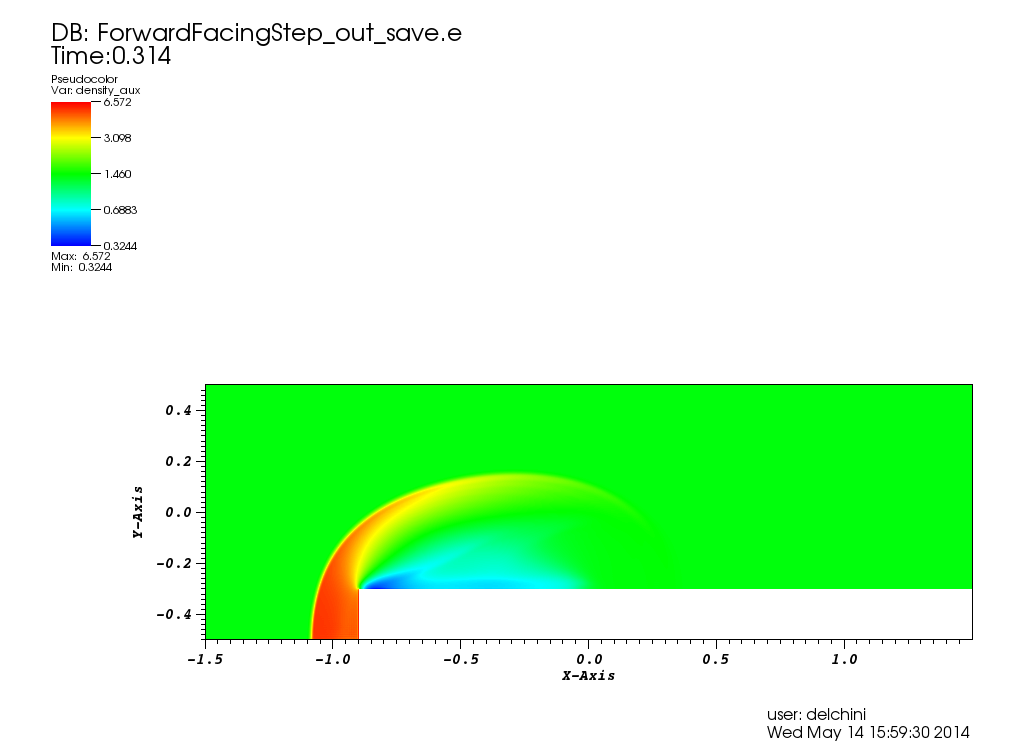
\includegraphics[scale=.50]{figures/FFSDensityEqualTo0p314.png}
\caption{Density solution at $t=0.314$ $s$.}
\label{fig:2d_ffs_rho_0314}
\end{figure}
%
\begin{figure}[H]
\centering
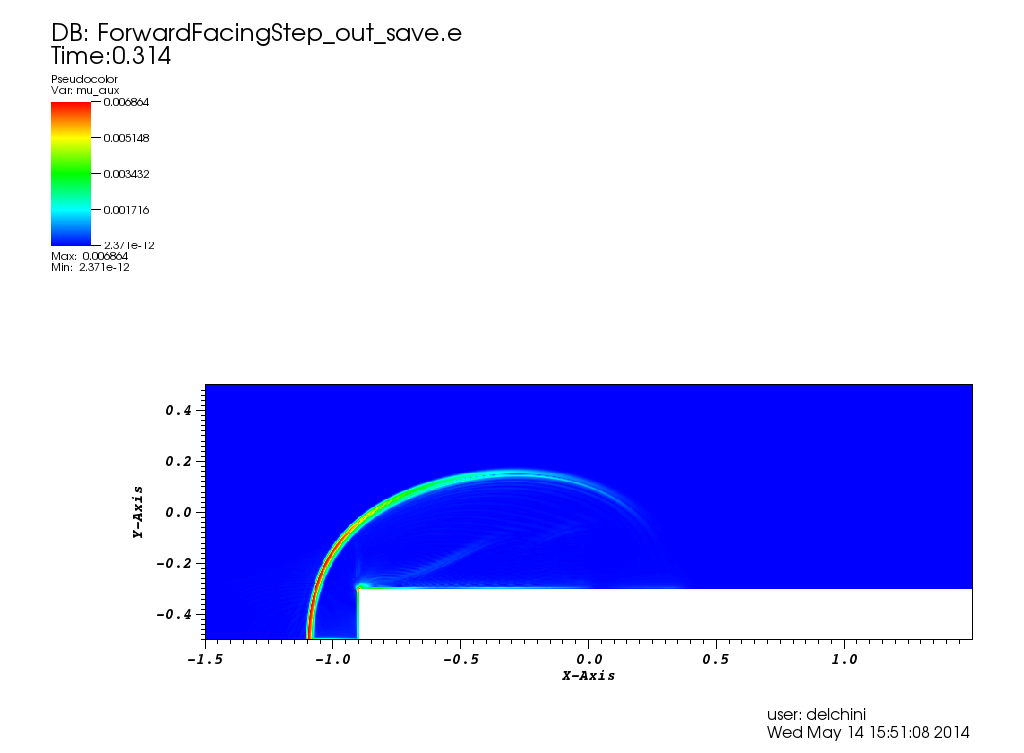
\includegraphics[scale=.50]{figures/FFSVisctEqualTo0p314.png}
\caption{Viscosity coefficient solution at $t=0.314$ $s$.}
\label{fig:2d_ffs_visc_0314}
\end{figure}
%
\begin{figure}[H]
\centering
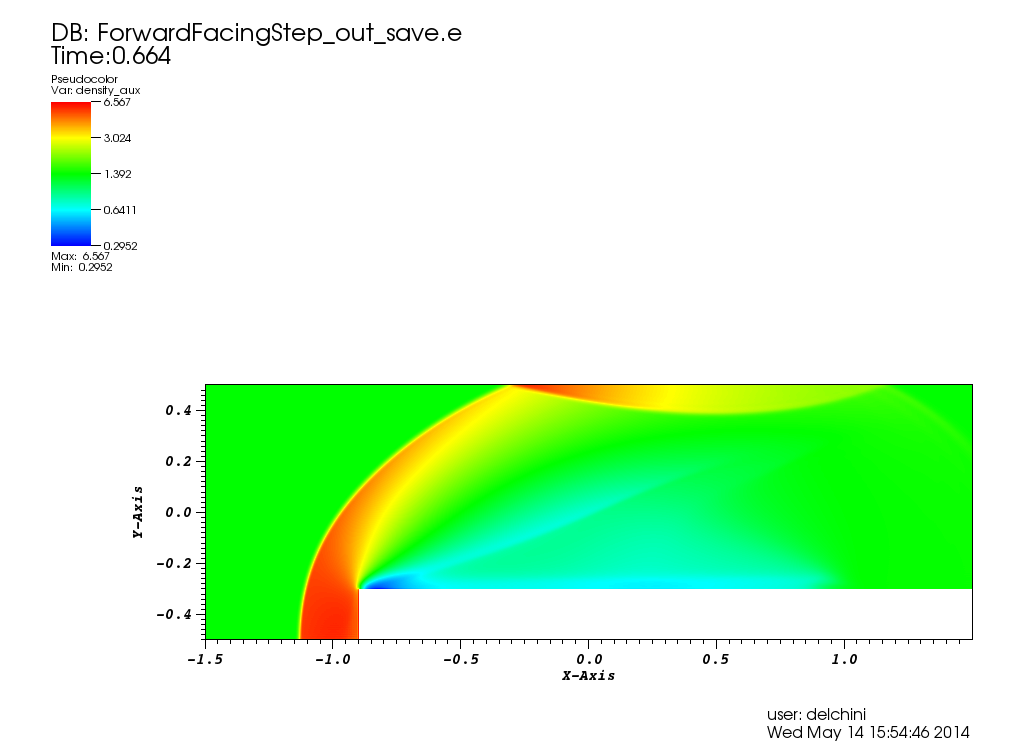
\includegraphics[scale=.50]{figures/FFSDensityEqualTo0p664.png}
\caption{Density solution at $t=0.664$ $s$.}
\label{fig:2d_ffs_rho_0664}
\end{figure}
%
\begin{figure}[H]
\centering
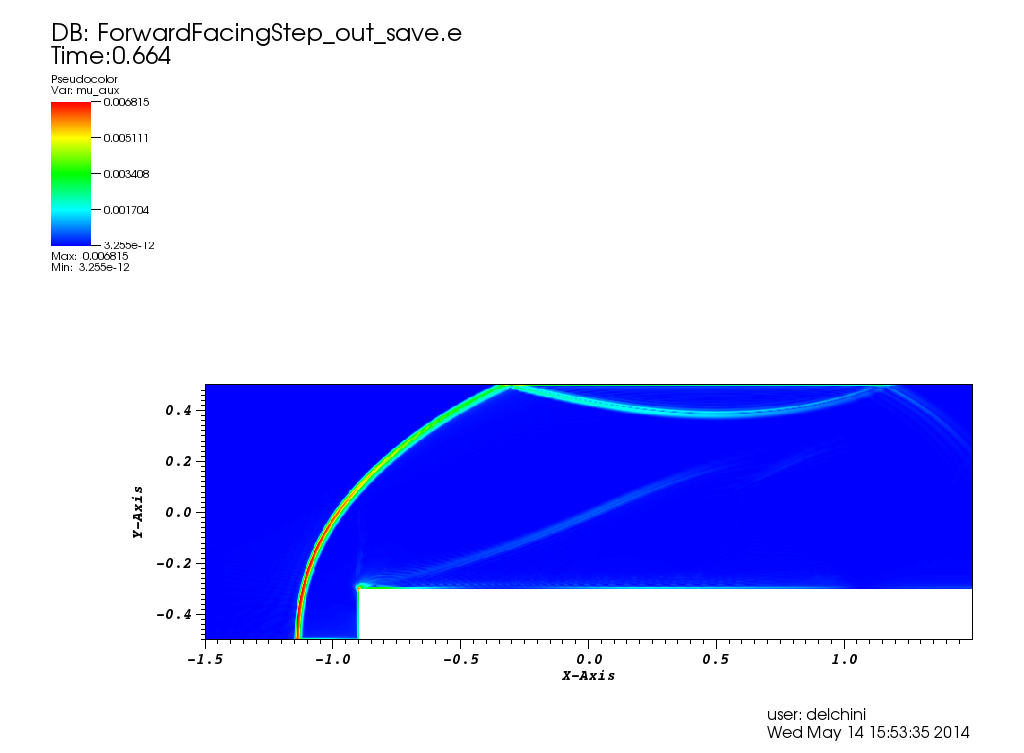
\includegraphics[scale=.50]{figures/FFSViscEqualTo0p664.png}
\caption{Viscosity coefficient solution at $t=0.664$ $s$.}
\label{fig:2d_ffs_visc_0664}
\end{figure}
%
\begin{figure}[H]
\centering
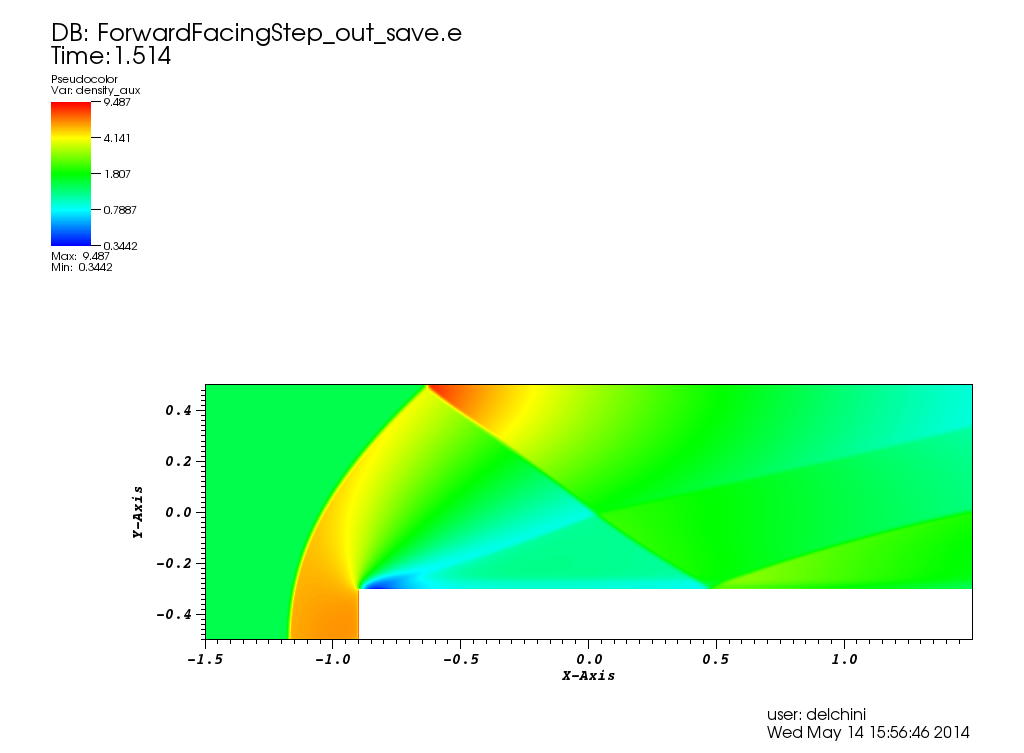
\includegraphics[scale=.50]{figures/FFSDensityEqualTo1p514.png}
\caption{Density solution at $t=1.514$ $s$.}
\label{fig:2d_ffs_rho_1514}
\end{figure}
%
\begin{figure}[H]
\centering
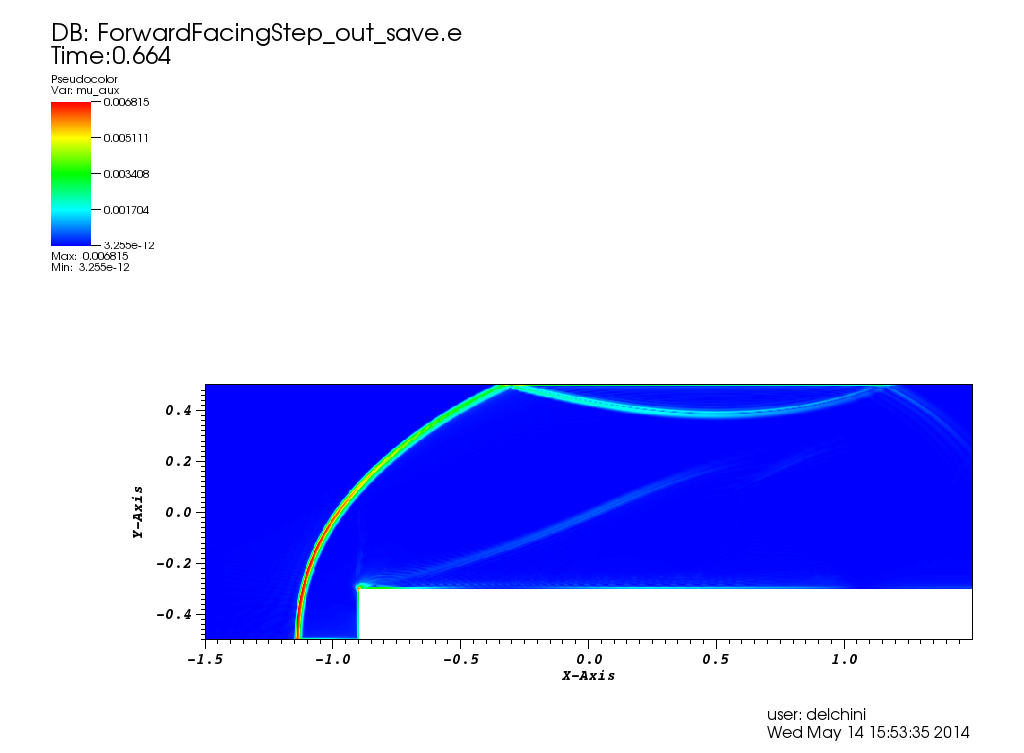
\includegraphics[scale=.50]{figures/FFSViscEqualTo0p664.png}
\caption{Viscosity coefficient solution at $t=1.514$ $s$.}
\label{fig:2d_ffs_visc_1514}
\end{figure}
%
\begin{figure}[H]
\centering
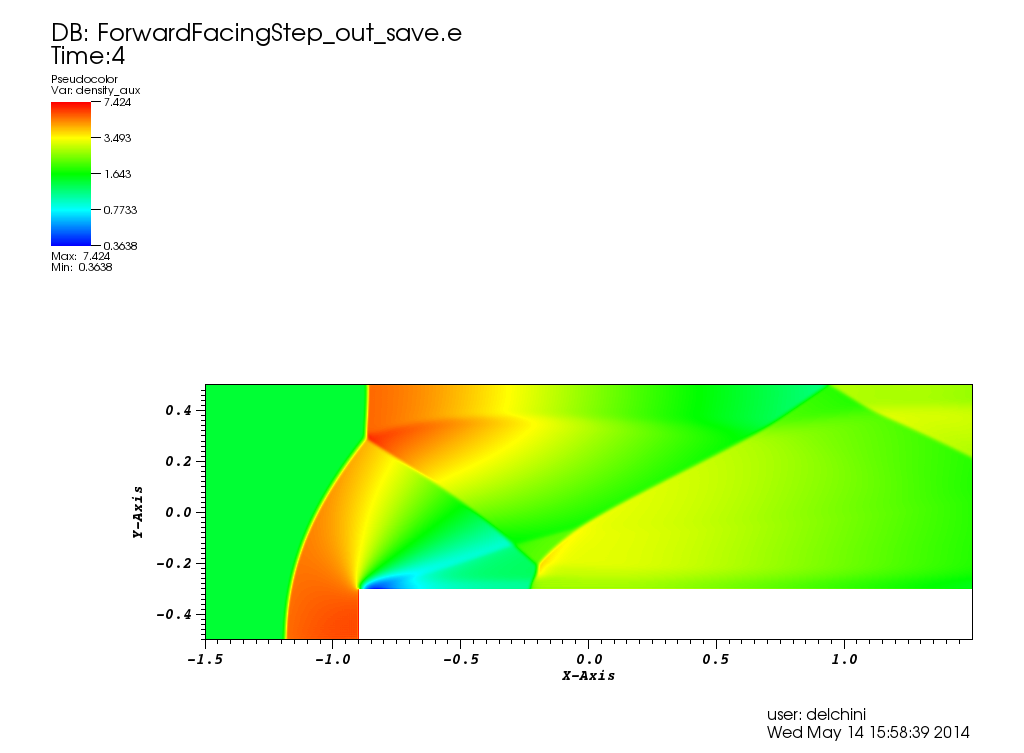
\includegraphics[scale=.50]{figures/FFSDensityEqualTo4.png}
\caption{Density solution at $t=4$ $s$.}
\label{fig:2d_ffs_rho_4}
\end{figure}
%
\begin{figure}[H]
\centering
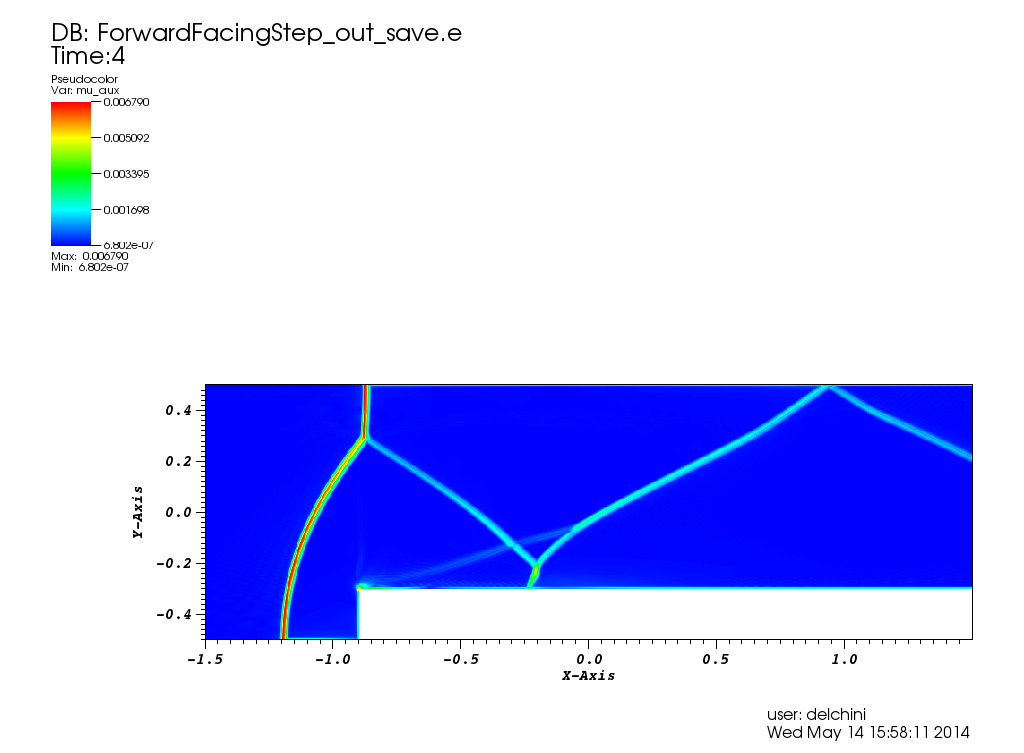
\includegraphics[scale=.50]{figures/FFSViscEqualTo4.png}
\caption{Viscosity coefficient solution at $t=4$ $s$.}
\label{fig:2d_ffs_visc_4}
\end{figure}
The numerical solution of the density at $t=4$ $s$ compares well to the ones obtained in (REFS), as least in a visual norm. The triple-point feature and the contact wave emerging from it are well resolved even if no Kelvin-Helmotz instability is observed (REF). It is also noticed that a significant amount of entropy is produced near the corner region. This is due to the corner singularity and this phenomenon is well documented (REFS). This artifact can be treated either by using special boundary condition to the corner since its normal vector is not defined, or by aggressively refining the mesh in the singularity region, or lastly, by modifying the geometry and use a round corner. 
%---------------------------------------------------------------------------------------------------
\subsection{Riemann problem number 12:} \label{sec:2d-riemann-pb-12}
%---------------------------------------------------------------------------------------------------
Riemann problem number $12$ (REF) is a popular $2$-D benchmark that is known to develop contact and shock waves, as well as fine structures. The computational domain $\Omega = (0,1)^2$ is initialized with four square regions. In each region a different set of initial values is set as follows:
\begin{equation}
\left\{
\begin{array}{cccc}
\rho = 4/5, & \vec{u} = (0, 0) & P = 1 & \text{ for } x \in (0, 0.5) \text{ and } y \in (0, 0.5) \\
\rho = 1, & \vec{u} = (3/\sqrt(17), 0) & P = 1 & \text{ for } x \in (0, 0.5) \text{ and } y \in (0.5, 1) \\
\rho = 17/32, & \vec{u} = (0,3/\sqrt{17}) & P = 1 & \text{ for } x \in (0.5, 1) \text{ and } y \in (0, 0.5) \\
\rho = 17/32, & \vec{u} = (0, 0) & P = 2/5 & \text{ for } x \in (0.5, 1) \text{ and } y \in (0.5, 1) \\
\end{array}
\right. \nonumber
\end{equation}
The same equation of state as in \sect{sec:2d-forward-facing-step} is used. An uniform mesh of $400 \times 400 $ elements was used along with a $\mathbb Q_1$ continuous Galerkin finite element method and the second-order temporal integrator $BDF2$. The simulation is run until $t=0.25s$ with a $CFL$ of 1. The density and viscosity profiles are given in (FIGS). 
%---------------------------------------------------------------------------------------------------
\subsection{Supersonic flow in a compression corner} \label{sec:corner}
%---------------------------------------------------------------------------------------------------
This is an example of a supersonic flow over a wedge of angle $15^{\circ}$ where an oblique shock is generated at steady-state. The Mach number upstream of the shock is fixed to $M=2.5$. The initial conditions are uniform: the pressure and temperature are set to $P=101325$ $Pa$ and $T=300$ $K$, respectively. The initial velocity is computed from the upstream Mach number and using the Ideal Gas equation of state with the same parameters as in \sect{sec:hump}. The code is run until steady-state. An analytical solution for this supersonic flow is available and give the downstream to upstream pressure, entropy and Mach number ratios \cite{CompressionCorner}. The analytical and numerical ratios are given in see in \tbl{tbl:corner_exact_sol}, and are very close. The pressure and viscosity coefficient solution are given for different times in \fig{fig:2d_cpc_rho_055} - \fig{fig:2d_cpc_visc_stt}.
\begin{table}[H]
\begin{center}
 \caption{\label{tbl:corner_exact_sol} Analytical solution for the supersonic flow on an edge eat $15^{\circ}$ at $M=2.5$.}
 \begin{tabular}{|c|c|c|}
 \hline
   & analytical & numerical \\
    & downstream to upstream ratio & downstream to upstream ratio \\
 \hline
Pressure & 2.47 & 2.467\\
  \hline
Mach number  &  0.74 & 0.741\\
   \hline
  Entropy & 1.03 & 1.026\\ \hline 
\end{tabular}
\end{center}
\nonumber
\end{table}
The inlet is supersonic and therefore, the pressure, temperature and velocity are specified using Dirichlet boundary conditions. The outlet is also supersonic and none of the characteristics enter the domain through this boundary: the values will be computed by the implicit solver.
%\begin{figure}[H]
 %       \centering
           \begin{figure}[H]%{0.52\textwidth}
                \centering
                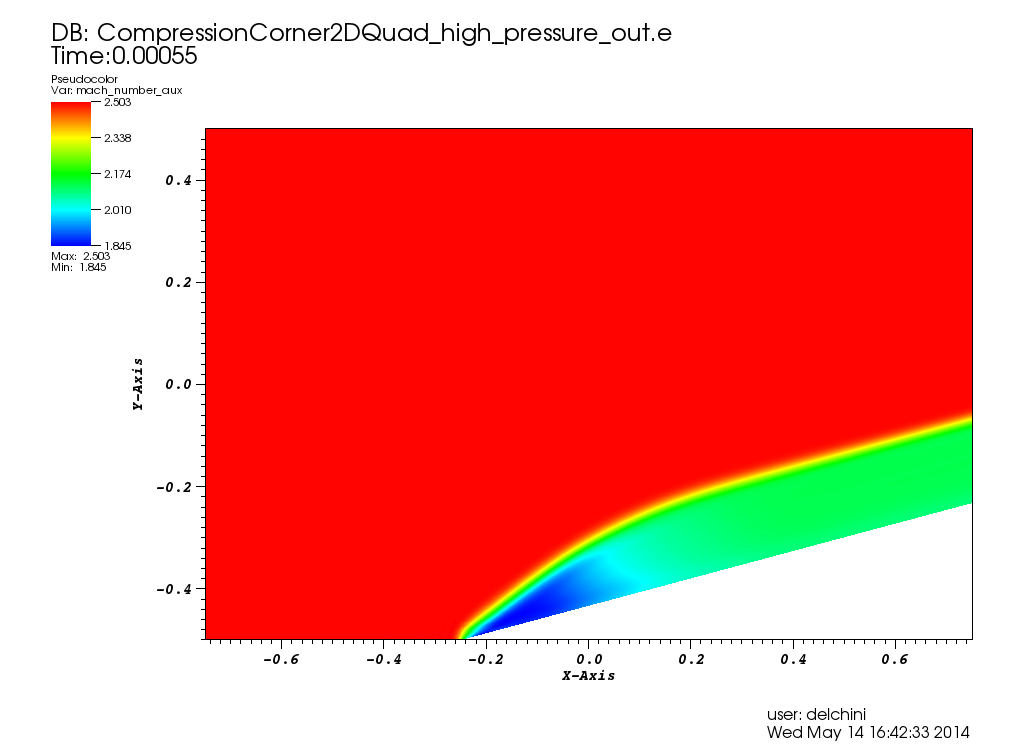
\includegraphics[scale=.50]{figures/CCDensityTime0p00055.png}
                \caption{Pressure solution at $t=5.5 \times 10^{-4}$.}
                \label{fig:2d_cpc_rho_055}
        \end{figure}%
          %add desired spacing between images, e. g. ~, \quad, \qquad etc. 
          %(or a blank line to force the subfigure onto a new line)
        \begin{figure}[H]%{0.52\textwidth}
                \centering
                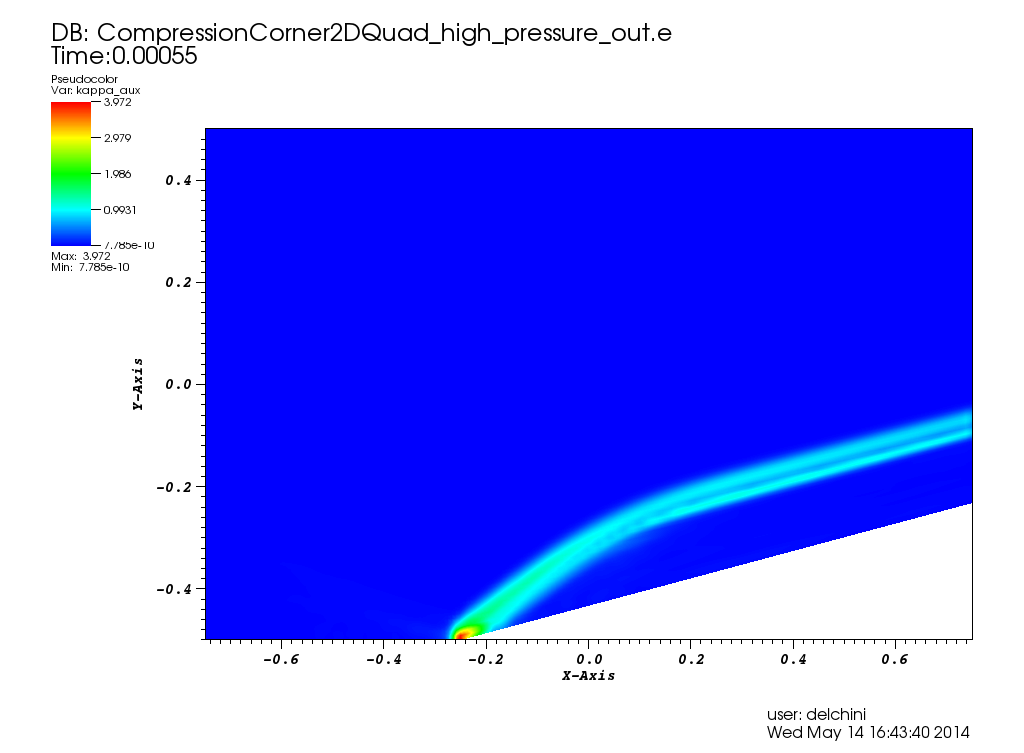
\includegraphics[scale=.50]{figures/CCViscosityTime0p00055.png}
                \caption{Viscosity coefficient at $t=5.5 \times 10^{-4}$.}
                \label{fig:2d_cpc_visc_055}
        \end{figure}
          \begin{figure}[H]%{0.52\textwidth}
                \centering
                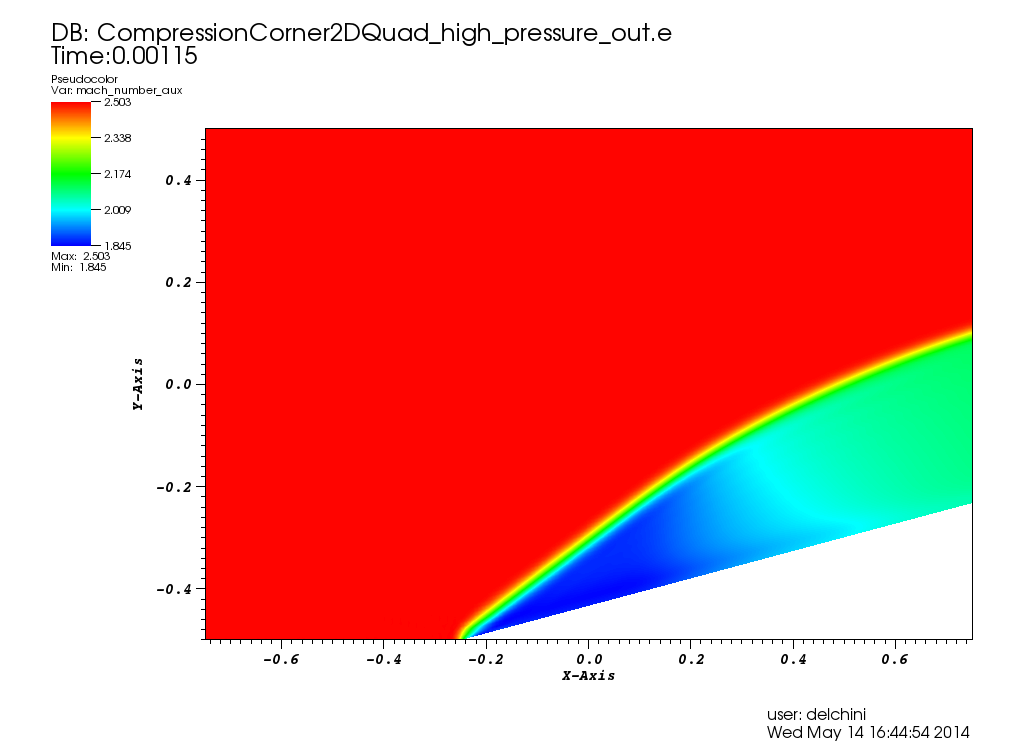
\includegraphics[scale=.50]{figures/CCDensityTime0p00115.png}
                \caption{Pressure solution at $t=1.15 \times 10^{-3}$.}
                \label{fig:2d_cpc_rho_115}
        \end{figure}%
          %add desired spacing between images, e. g. ~, \quad, \qquad etc. 
          %(or a blank line to force the subfigure onto a new line)
        \begin{figure}[H]%{0.52\textwidth}
                \centering
                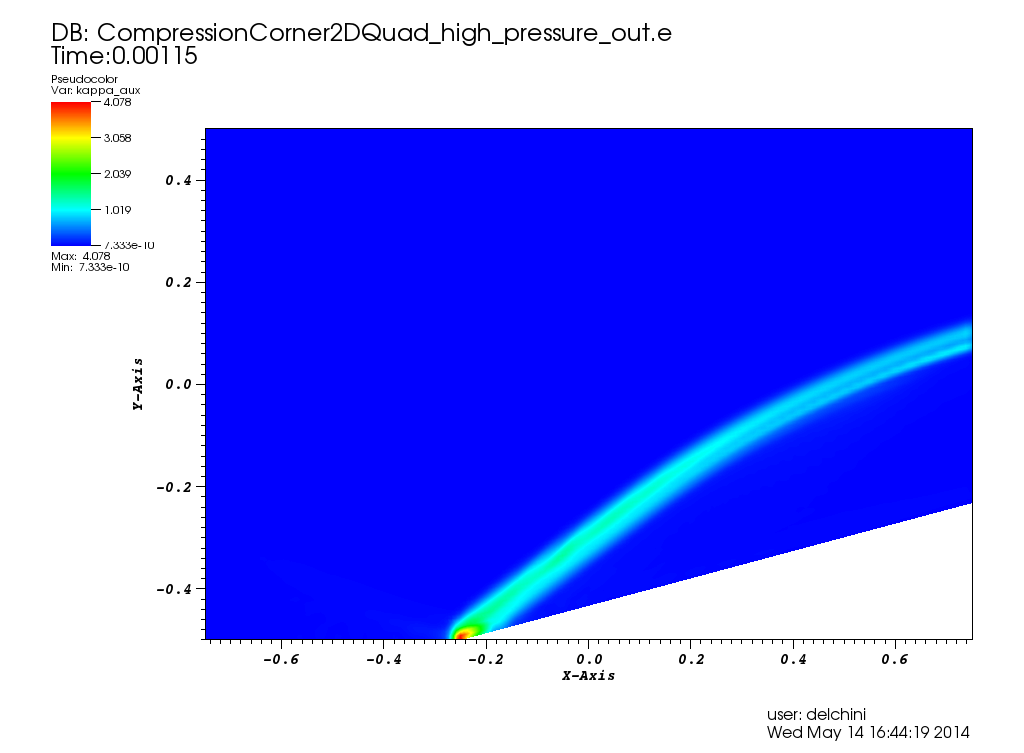
\includegraphics[scale=.50]{figures/CCViscosityTime0p00115.png}
                \caption{Viscosity coefficient at $t=1.15 \times 10^{-3}$.}
                \label{fig:2d_cpc_visc_115}
        \end{figure}
         \begin{figure}[H]%{0.52\textwidth}
                \centering
                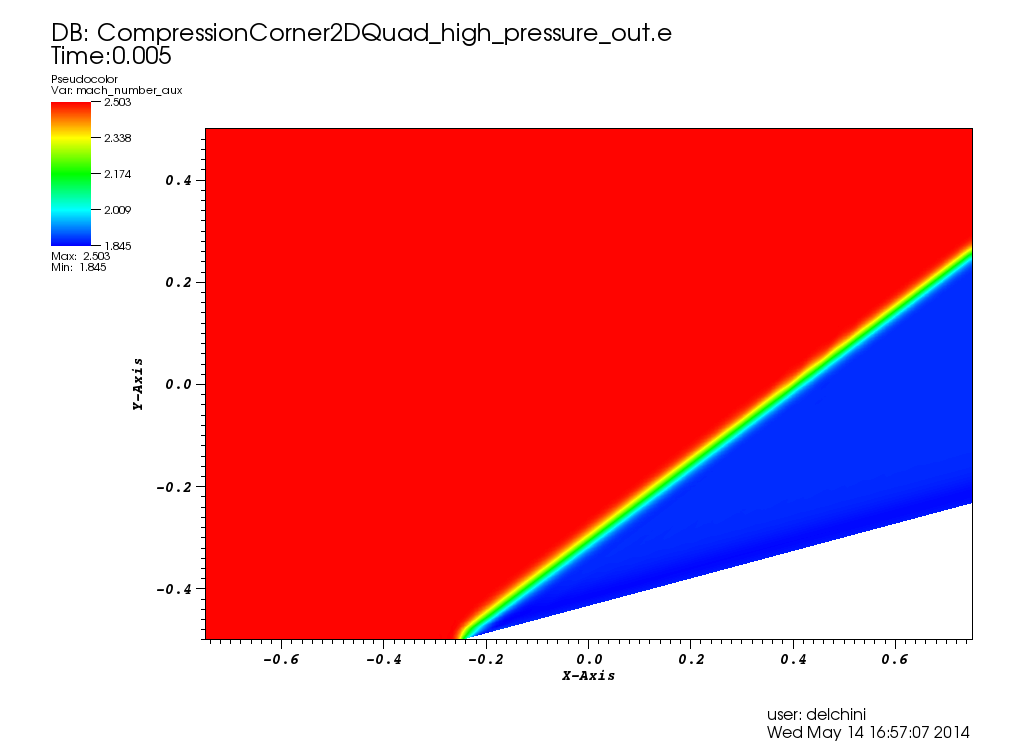
\includegraphics[scale=.50]{figures/CCDensityTimeStt.png}
                \caption{Pressure solution at steady-state.}
                \label{fig:2d_cpc_rho_stt}
        \end{figure}%
          %add desired spacing between images, e. g. ~, \quad, \qquad etc. 
          %(or a blank line to force the subfigure onto a new line)
        \begin{figure}[H]%{0.52\textwidth}
                \centering
                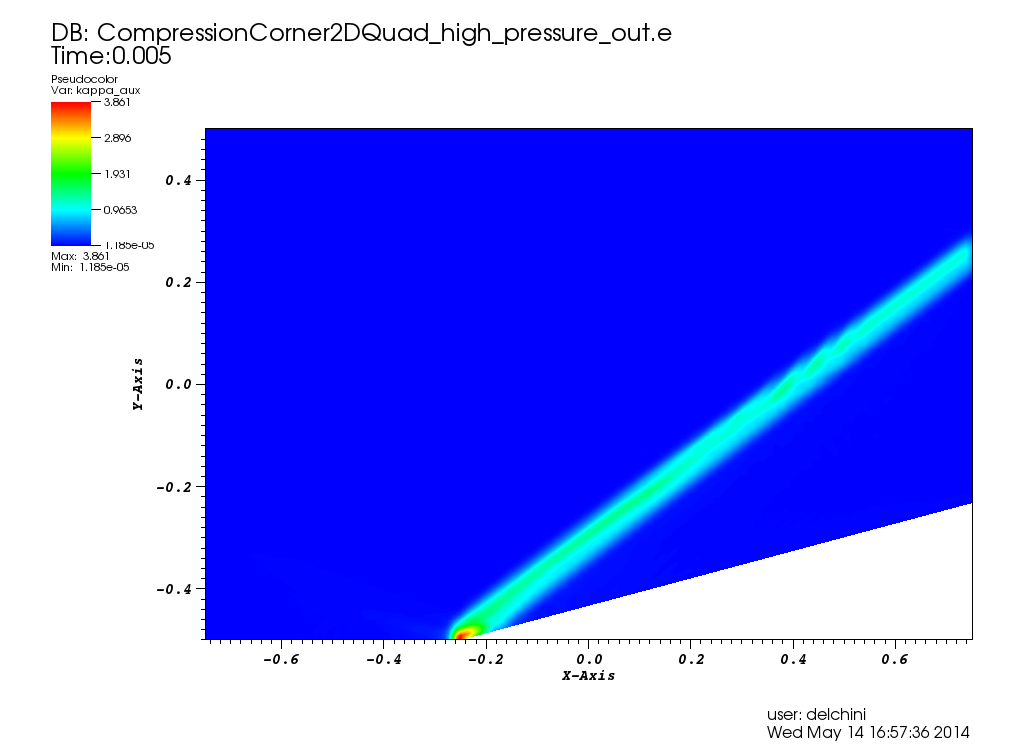
\includegraphics[scale=.50]{figures/CCViscosityTimeStt.png}
                \caption{Viscosity coefficient at steady-state.}
                \label{fig:2d_cpc_visc_stt}
        \end{figure}
From the above figures, it is observed that the solution is formed of two regions of constant state. During the transient, the shock moves from the bottom wall to its steady-state solution. The same variations are observed in viscosity coefficient solution. At steady-state, the viscosity coefficient is large in the shock region and small anywhere else and thus, behaves as expected. At the corner of the edge at $x=-0.25$ $m$, the viscosity coefficient is peaked because of the treatment of the wall boundary condition: at this particular node, the normal is not well defined and can cause numerical errors. 
        %add desired spacing between images, e. g. ~, \quad, \qquad etc. 
          %(or a blank line to force the subfigure onto a new line)
        \begin{figure}[H]%{0.49\textwidth}
                \centering
                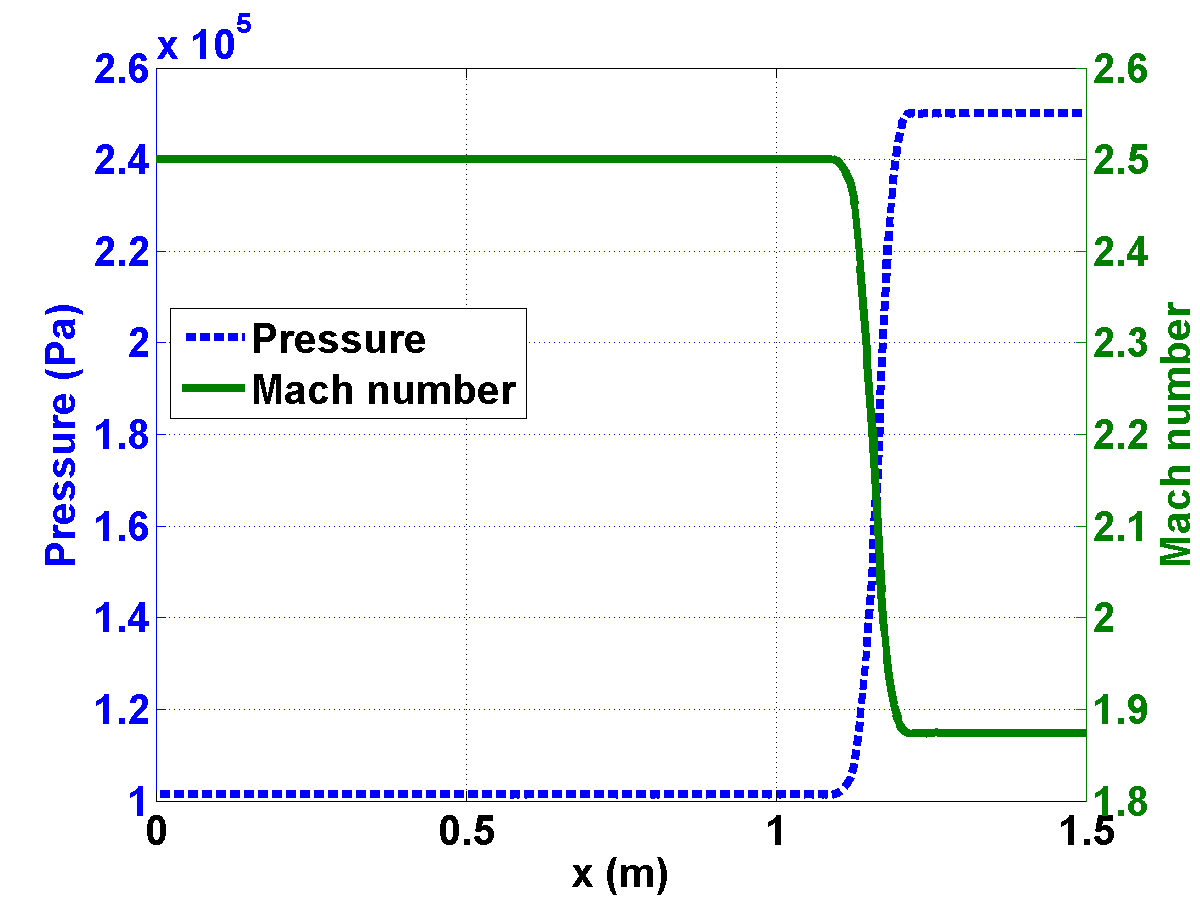
\includegraphics[scale=.50]{figures/mach_number_pressure.png}
                \caption{Pressure and Mach number profiles at steady-state}
                \label{fig:2d_corner_isomach}
        \end{figure}        
          %add desired spacing between images, e. g. ~, \quad, \qquad etc. 
          %(or a blank line to force the subfigure onto a new line)
        \begin{figure}[H]%{0.49\textwidth}
                \centering
                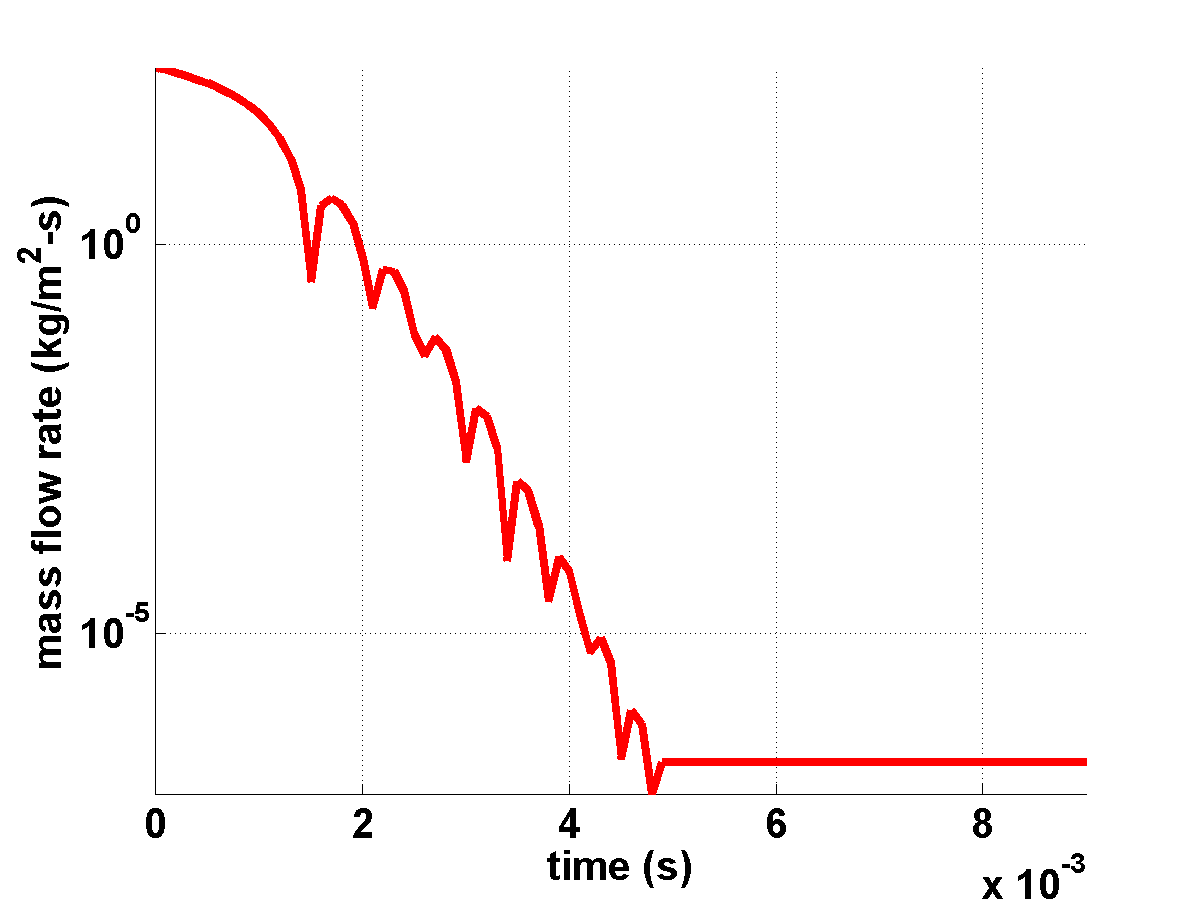
\includegraphics[scale=.50]{figures/CompressionCorner2DQ.png}
                \caption{Difference between inlet and outlet mass flow rates as a function of time.}
                \label{fig:2d_convergence}
        \end{figure}
%The steady-state numerical solution is given in \fig{fig:2d_corner}: the Mach number, the viscosity coefficients are plotted in \fig{fig:2d_corner_mach} and \fig{fig:2d_corner_visc}, respectively. The steady-state solution is formed of two regions of constant states, separated by the oblique shock. In \fig{fig:2d_corner_visc}, the viscosity coefficient is large in the shock, small anywhere else, and thus, behaves as expected. 
The $1$-D plots of the pressure and the mach number at $y=0$, are also given in \fig{fig:2d_corner_isomach}: the shock does not show any spurious oscillations and is well resolved. Finally, the difference between the inlet and outlet mass flow rates is plotted in \fig{fig:2d_convergence} and show that a steady-state is reached. \\
Overall, the numerical solution does not show any oscillations, match the analytical solution, and the shock is well resolved.
%---------------------------------------------------------------------------------------------------
\subsection{Supersonic flow over a $5^\circ$ double-wedge obstruction:} \label{sec:double_wedge}
%---------------------------------------------------------------------------------------------------
The last of the $2$-D supersonic example that is proposed to study is a Mach$2,5$ flow over a double-wedge obstruction located on the lower wall. The interesting feature of this test is that a steady-state is reached. The geometry used is shown in (FIG) and was discretized with $4000$ $\mathbb Q_1$ elements. The double wedge extends on the bottom boundary from $x=1$ to $x=5$  $m$. The top wall is located at $y=5$ $m$. A supersonic inlet boundary condition was set at the inlet by specifying the pressure, $P=101,325$ $Pa$, the temperature, $T=300$ $K$ and the vector velocity $\vec{u} = (868.032, 0)$ $m \cdot s^{-1}$. The wall-boundary and supersonic outlet boundary conditions were implemented following the method described in (SECTION BCS). The second-order temporal integrator $BDF2$ was used with a $CFL$ of 5 to reach the steady-state that was detected by monitoring the norm of the total residual. The Ideal gas equation of state was used with an adiabatic constant $\gamma = 1.4$ and a volumetric heat capacity $C_v = 716.7$ $J \cdot K^{-1}$ (air properties). The Mach number and viscosity coefficients profiles at steady-state are given in \fig{fig:2d_dbwd_stt} and \fig{fig:2d_dbw_visc_stt}, respectively. 
        \begin{figure}[H]%{0.52\textwidth}
                \centering
                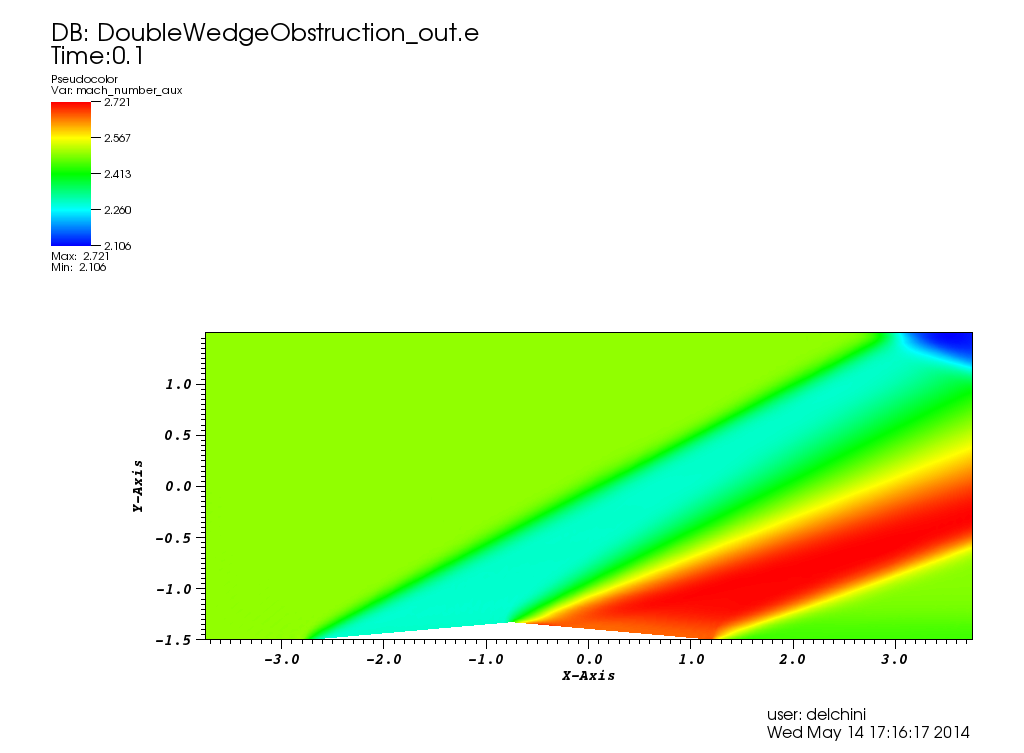
\includegraphics[scale=.50]{figures/DWOMachNumberStt.png}
                \caption{Pressure solution at steady-state.}
                \label{fig:2d_dbwd_stt}
        \end{figure}%
%
        \begin{figure}[H]%{0.52\textwidth}
                \centering
                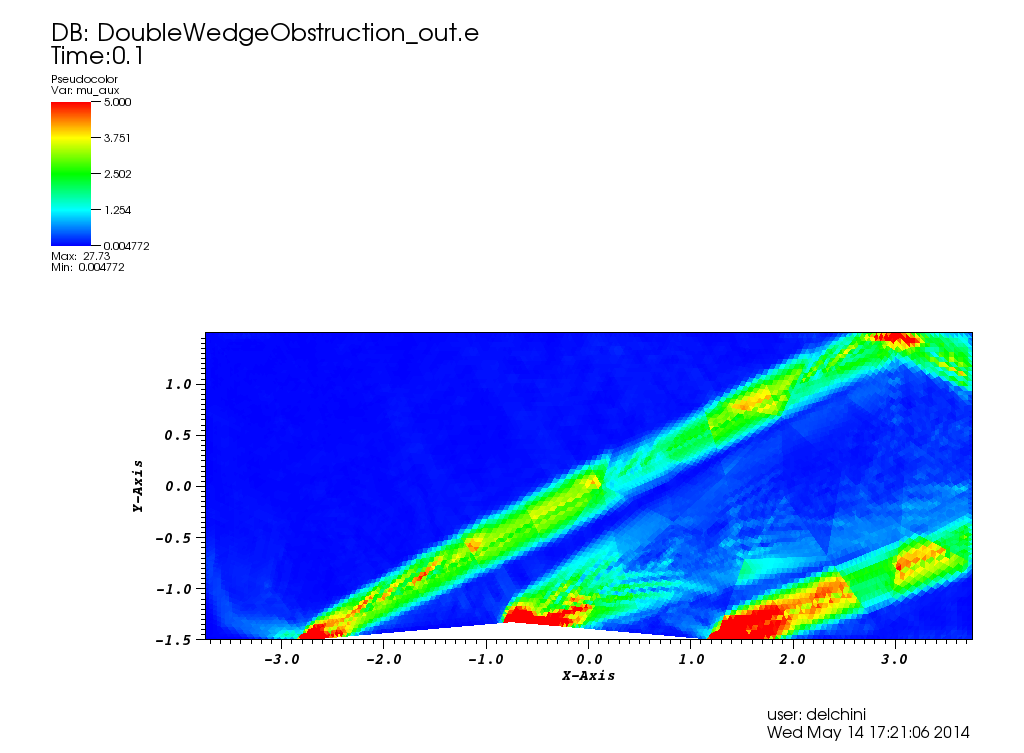
\includegraphics[scale=.50]{figures/DWOViscosityStt.png}
                \caption{Viscosity coefficient at steady-state.}
                \label{fig:2d_dbw_visc_stt}
        \end{figure}
The stay-state solution consists of a two shocks that form because of the interaction of the flow with the double wedge. The first wedge generates a shock that reflects on the top wall and then exits the computational domain: the interaction of the shock with the wall close to the outlet boundary requires a robust implentation of the boundary conditions and the stabilization method. The second shock is generated by the trailing wedge. In between the two shock regions, an expansion fan is formed. 
%%%%%%%%%%%%%%%%%%%%%%%%%%%%%%%%%%%%%%%%%%%%%%%%%%%%%%%%%%%%%%%%%%%%%%%%%%%%%%%%%%%%%%%%%%%%%%%%%%%%
%%%%%%%%%%%%%%%%%%%%%%%%%%%%%%%%%%%%%%%%%%%%%%%%%%%%%%%%%%%%%%%%%%%%%%%%%%%%%%%%%%%%%%%%%%%%%%%%%%%%
\section{$2$-D numerical results for subsonic flows:} \label{sec:2d-susubsonic-results}
%%%%%%%%%%%%%%%%%%%%%%%%%%%%%%%%%%%%%%%%%%%%%%%%%%%%%%%%%%%%%%%%%%%%%%%%%%%%%%%%%%%%%%%%%%%%%%%%%%%%
%%%%%%%%%%%%%%%%%%%%%%%%%%%%%%%%%%%%%%%%%%%%%%%%%%%%%%%%%%%%%%%%%%%%%%%%%%%%%%%%%%%%%%%%%%%%%%%%%%%%
%---------------------------------------------------------------------------------------------------
\subsection{Subsonic flow over a 2-D cylinder} \label{sec:cylinder}
%---------------------------------------------------------------------------------------------------
Fluid flow over a 2-D cylinder is often used as a benchmark case to test numerical schemes in the low-Mach regime \cite{LowMach1, LowMach2, LowMach3}. For this test, an analytical solution is available in the incompressible limit or low-Mach limit and is often referred to as the potential flow solution. The main features of the potential flow are the following:
%
\begin{itemize}
\item The solution is symmetric: the iso-Mach contour lines are used to asses the symmetry of the numerical solution;
\item The velocity at the top of the cylinder is twice the incoming velocity set at the inlet;
\item The pressure fluctuations are proportional to the square of inlet Mach number, i.e., 
\begin{equation}
\delta P = \frac{\max(P(\vec{r})) - \min(P(\vec{r}))}{\max(P(\vec{r}))}  \propto M_\infty^2
%||\tilde{\vec{u}}|| = \frac{\max(||\vec{u}||) - \min(||\vec{u}||)}{\max(||\vec{u}||)}  \propto M_\infty\nonumber 
\end{equation}
where $\delta P$ and $M_\infty$ denote the pressure fluctuations and the inlet Mach number, respectively.
\end{itemize}
%
The computational domain consists of a $1\times 1$ square with a circular hole of radius $0.05$ in its center. A $\mathbb{P}_1$ triangular mesh with $4008$ triangular elements was used to discretize the geometry. The ideal gas equation of state, with $\gamma=1.4$ is used. At the inlet, a subsonic stagnation boundary condition is used: the stagnation pressure and temperature are computed using the following relations:
%
\begin{equation}
\label{eq:stagnation_relations}
\left\{
\begin{array}{l}
P_0 = P\left( 1 + \frac{\gamma-1}{2} M^2 \right)^{\frac{\gamma-1}{\gamma}} \\
T_0 = T\left( 1 + \frac{\gamma-1}{2} M^2 \right)
\end{array}
\right.
\end{equation}
%
An static pressure boundary condition is used for the outlet boundary and the following static pressure $P_s = 101,325$ $Pa$ is set. The implementation of the pressure boundary conditions is based of \cite{SEM}. A solid wall boundary condition is set for the top and bottom walls of the computational domain. The simulations are run until a steady state is reached with a $CFL$ of $40$. The steady state is considered reached when the residual norm  (for all equations) is less than $10^{-12}$.

Several simulations are performed, with inlet Mach numbers $M_{\text{inlet}}$ ranging from $10^{-3}$ to $10^{-7}$, and are shown from \fig{fig:cyl_1em3} through \fig{fig:cyl_1em7}. The iso-Mach contour lines are drawn using 30 equally-spaced intervals $2 \ 10^{-10}$ to $M_{\text{inlet}}$ and allow us to assess the symmetry of the numerical solution.
%
%\begin{figure}[H]
%        \centering
        \begin{figure}[H]
                \centering
                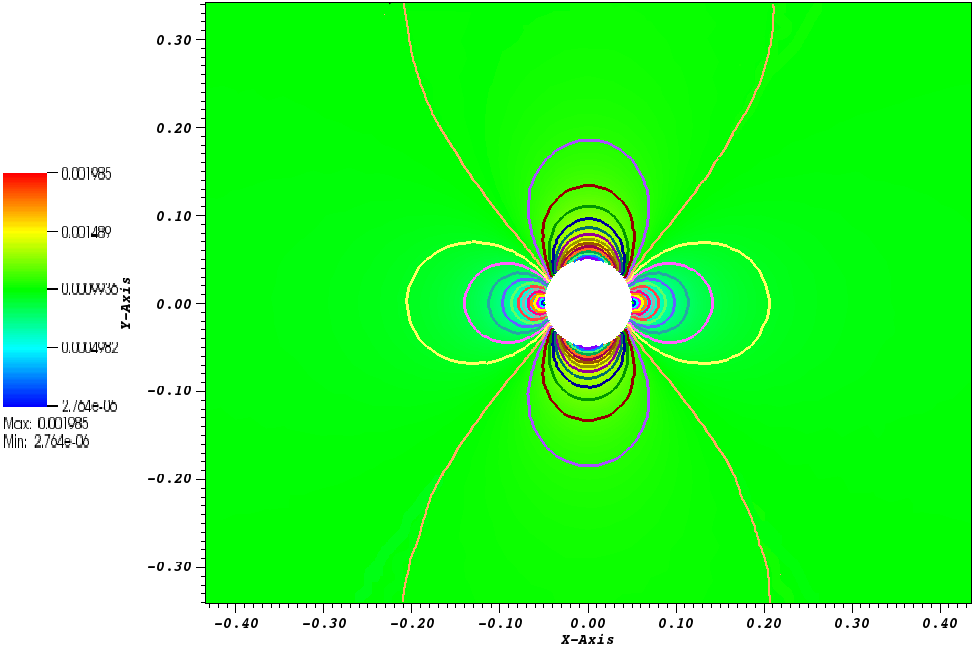
\includegraphics[width=\textwidth]{figures/CylinderMach1em3ZoomIn.png}
                \caption{$M_{\text{inlet}}=10^{-3}$}
                \label{fig:cyl_1em3}
        \end{figure}%

        \begin{figure}[H]
                \centering
                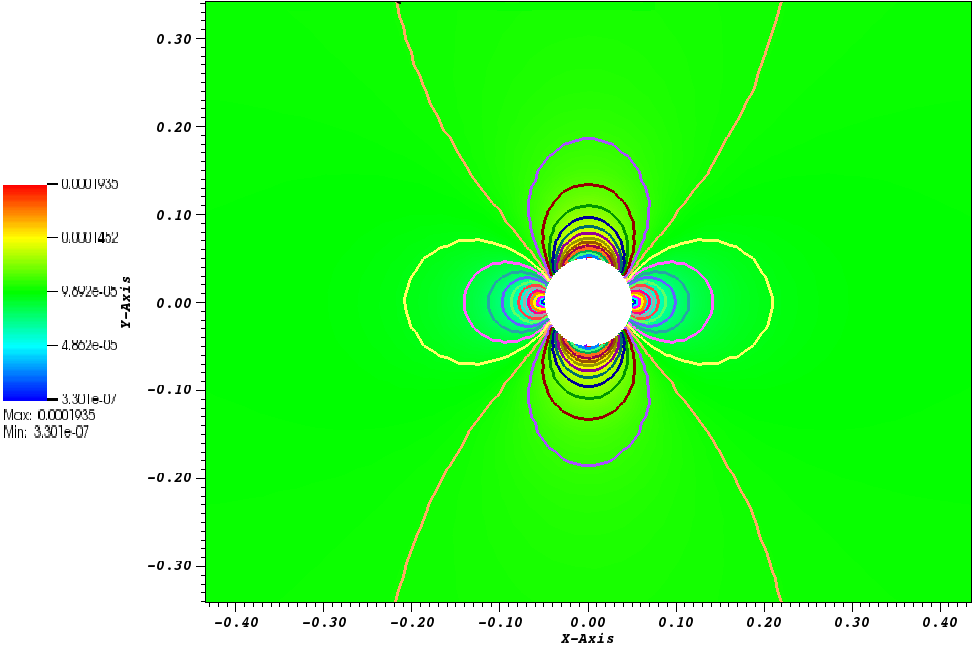
\includegraphics[width=\textwidth]{figures/CylinderMach1em4ZoomIn.png}
                \caption{$M_{\text{inlet}}=10^{-4}$}
                \label{fig:cyl_1em4}
        \end{figure}    

        \begin{figure}[H]
                \centering
                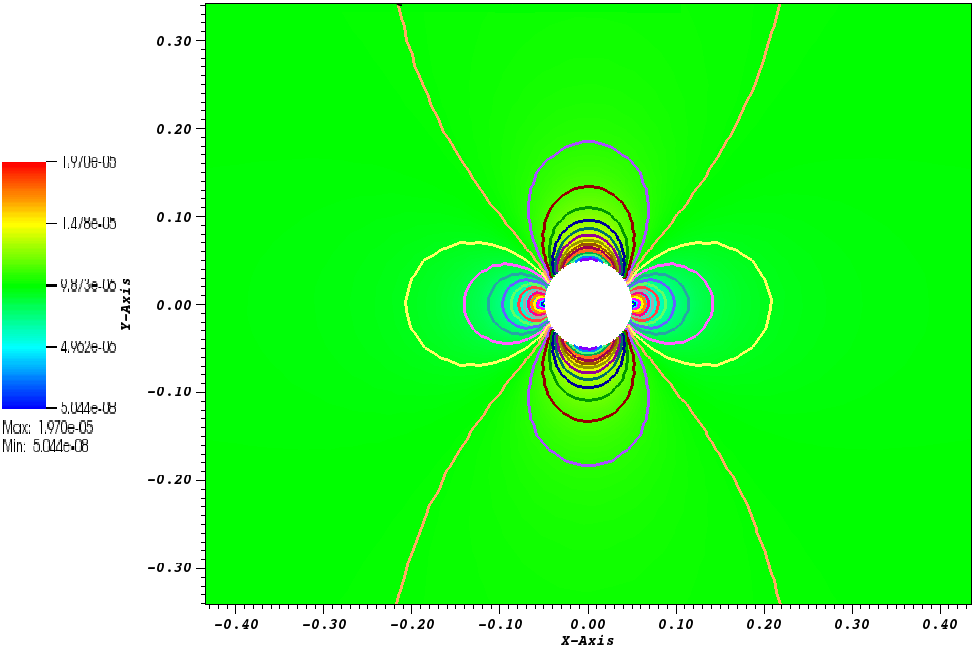
\includegraphics[width=\textwidth]{figures/CylinderMach1em5ZoomIn.png}
                \caption{$M_{\text{inlet}}=10^{-5}$}
                \label{fig:cyl_1em5}
        \end{figure}

        \begin{figure}[H]
                \centering
                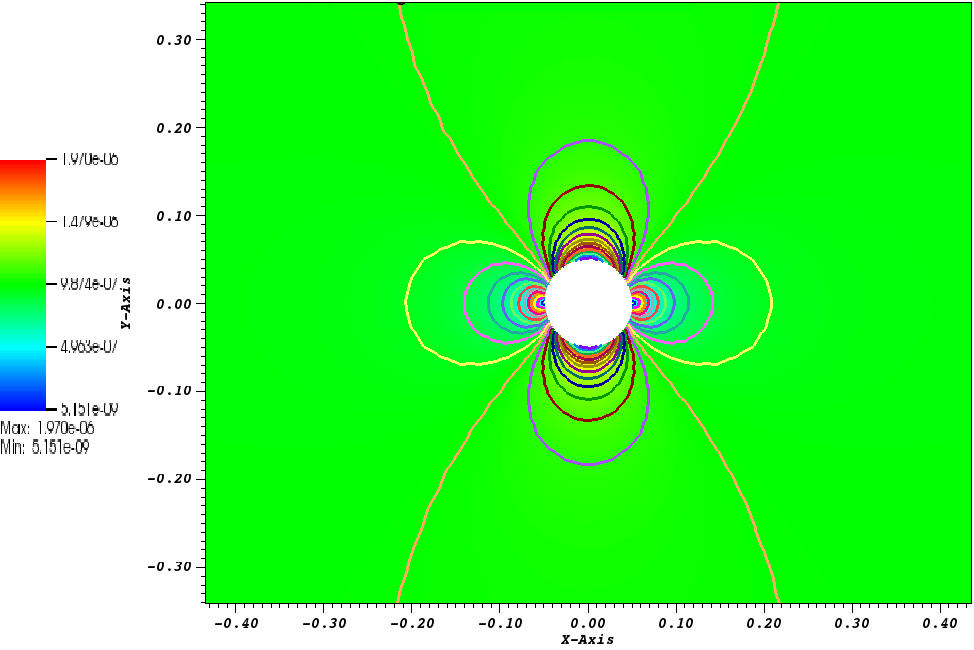
\includegraphics[width=\textwidth]{figures/CylinderMach1em6ZoomIn.png}
                \caption{$M_{\text{inlet}}=10^{-6}$}
                \label{fig:cyl_1em6}
        \end{figure}

        \begin{figure}[H]
                \centering
                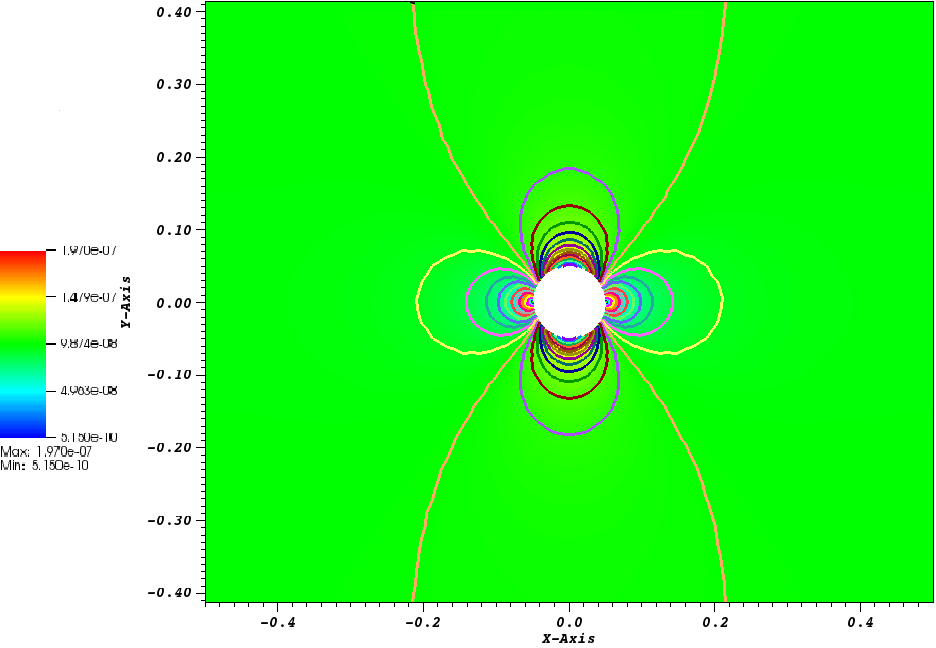
\includegraphics[width=\textwidth]{figures/CylinderMach1em7ZoomIn.png}
                \caption{$M_{\text{inlet}}=10^{-7}$}
                \label{fig:cyl_1em7}
        \end{figure}
%        \caption{Iso-Mach lines for a subsonic flow over a 2-D cylinder with inlet Mach number values from ranging from $10^{-3}$ to $10^{-7}$ (steady-state solution).}
%				\label{fig:cylinder}
%\end{figure}
%
The velocity at the top of the cylinder and at the inlet are given for different Mach-number values (ranging from $10^{-3}$ to $10^{-7}$) in \tbl{tbl:velocity_ratio}. The ratio of the inlet velocity to the velocity at the top of cylinder is also computed and is very close to the theoretical value of $2$ that is expected in the incompressible limit.
%
\begin{table}[H]
\begin{center}
 \caption{\label{tbl:velocity_ratio}Velocity ratio for different Mach numbers.}
\begin{tabular}{|c|c|c|c|}
\hline
Mach number & inlet velocity & velocity at the top of the cylinder & ratio \\ \hline
$10^{-3}$ & $2.348$ $10^{-3}$ & $1.176$ $10^{-3}$& $1.99$  \\ \hline
$10^{-4}$ & $2.285$ $10^{-4}$ & $1.145$ $10^{-4}$& $1.99$  \\ \hline
$10^{-5}$ & $2.283$ $10^{-5}$ & $1.144$ $10^{-5}$ & $1.99$ \\ \hline
$10^{-6}$ & $2.283$ $10^{-6}$ & $1.144$ $10^{-6}$ & $1.99$ \\ \hline
$10^{-7}$ & $2.283$ $10^{-7}$ & $1.144$ $10^{-7}$ & $1.99$ \\ \hline
\end{tabular}
\end{center}
\nonumber
\end{table}
%
In \fig{fig:pressure_vel_fluc}, the fluctuations in pressure and velocity are plotted as a function of the Mach number (on a log-log scale). The fluctuations are expected to be of the order of $M^2$ and $M$ for the pressure and velocity, respectively. It is known that some stabilization methods, e.g., \cite{LowMach1, LowMach2, LowMach3}, can produce pressure fluctuations with the wrong Mach-number order. Here, entropy viscosity method yields the correct order in the low-Mach limit. For ease of comparison, the reference lines with slope values of 1 and 2 are also plotted.
%
\begin{figure}[H]
\centering
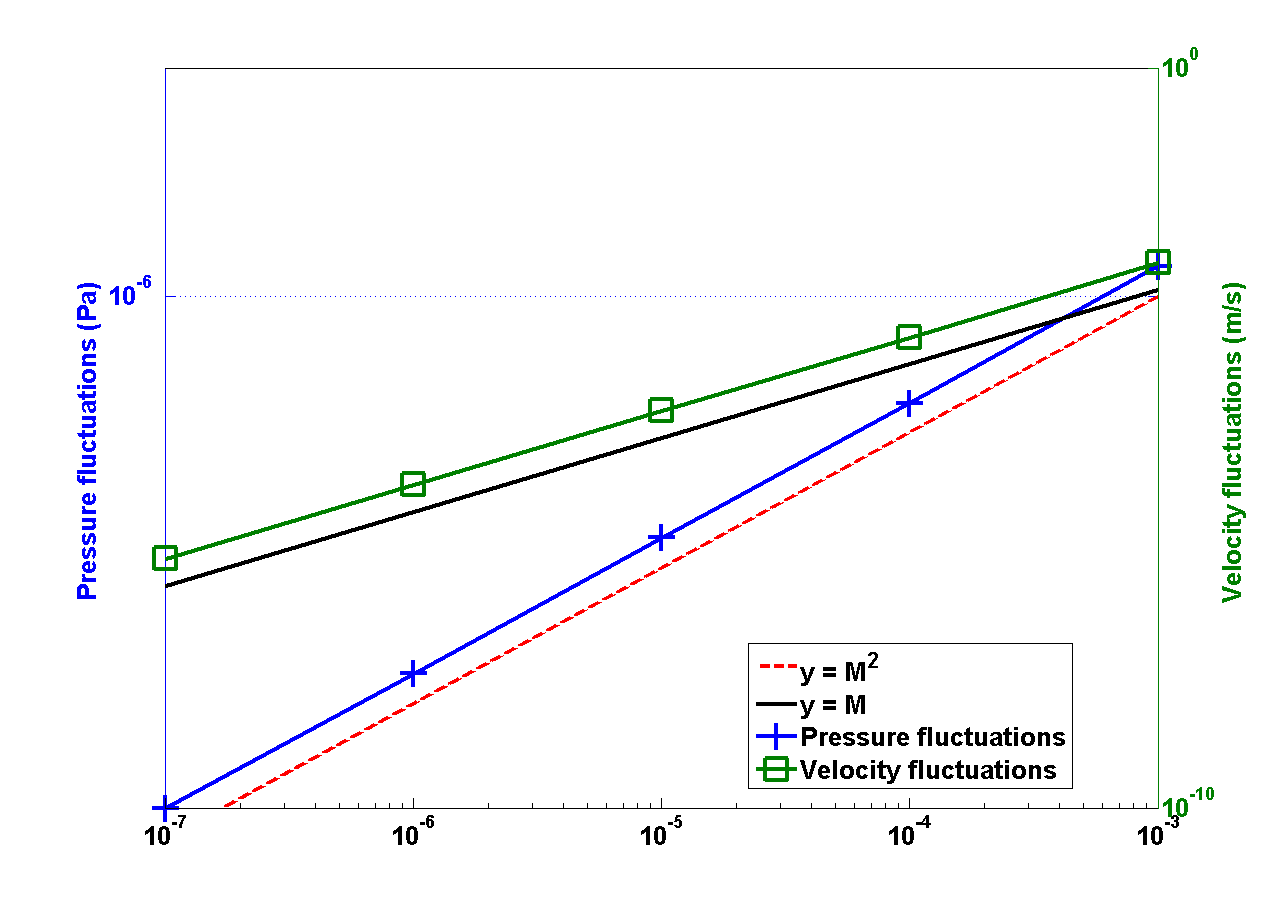
\includegraphics[width=\textwidth]{figures/pressure_fluctuation.png}
\caption{Log-log plot of the pressure and velocity fluctuations as a function of the far-field Mach number.}
\label{fig:pressure_vel_fluc}
\end{figure}

%---------------------------------------------------------------------------------------------------
\subsection{Subsonic flow over a 2-D hump} \label{sec:hump}
%---------------------------------------------------------------------------------------------------
%\tcr{Is it a circular hump or Gaussian hump in the literature???} \tcb{circular hump}
This is a another example of an internal flow configuration. It consists of a channel of height $L=1$ $m$ and length $3L$, with a circular bump of length $L$ and thickness $0.1L$. The bump is located on the bottom wall at a distance $L$ from the inlet. The system is initialized with an uniform pressure $P=101,325$ $Pa$ and temperature $T=300$ $K$. The initial velocity is computed from the inlet Mach number, the pressure, the temperature and the ideal gas equation (with  $\gamma=1.4$). Here,  $C_v = 717$ $J/kg-K$. At the inlet, a subsonic stagnation boundary condition is used and the stagnation pressure and temperature are computed using \eqt{eq:stagnation_relations}.
The static pressure $P_s = 101,325$ $Pa$ is set at the subsonic outlet. The results are shown in \fig{fig:2d_hump_mach_0p7}, \fig{fig:2d_hump_mach_0p01}, \fig{fig:2d_hump_mach_0p0001} and \fig{fig:2d_hump_mach_0p0000001} for the inlet Mach numbers $M_{\infty}=0.7$, $M_{\infty}=0.01$, $M_{\infty}=10^{-4}$ and $M_{\infty}=10^{-7}$, respectively. It is expected that, within the low Mach number range, the solution does not depend on the Mach number and is identical to the solution obtained with an incompressible flow code. On the other hand, for a flow at $M=0.7$, the compressible effects become more important and shock can form. An uniform grid of $3352$ $Q_1$ elements was used to obtain the numerical solution for Mach numbers below $M_{\infty}=0.01$. A once-refined mesh was employed for the $M_{\infty}=0.7$ simulation in order to better resolve the shock. A $CFL$ of 20 was employed and the simulations were run until steady state.
%
%\begin{figure}[H]
%        \centering
        \begin{figure}[H]
                \centering
                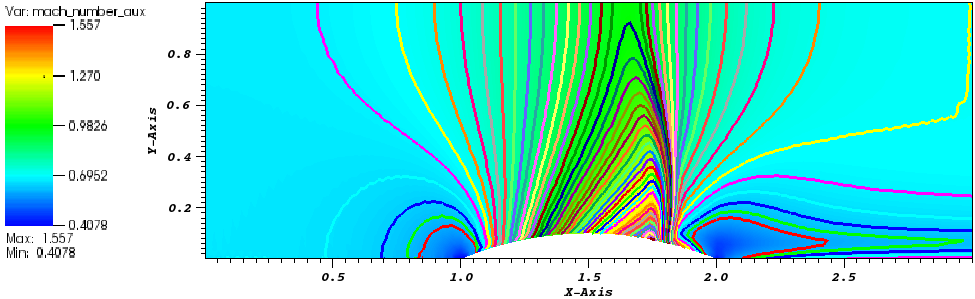
\includegraphics[width=\textwidth]{figures/Hump2D_mach_0p7.png}
                \caption{Mach $0.7$}
                \label{fig:2d_hump_mach_0p7}
        \end{figure}%

        \begin{figure}[H]
                \centering
                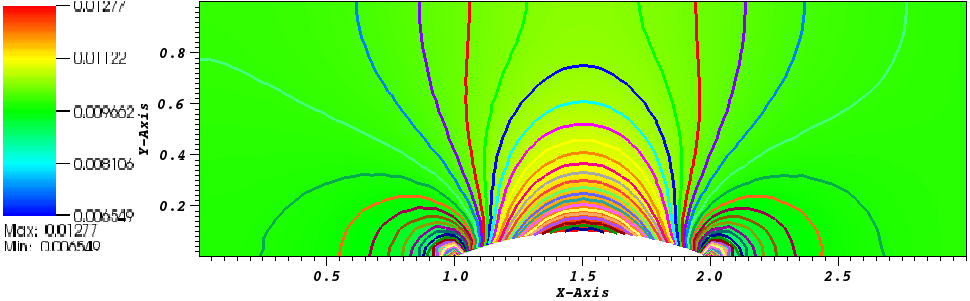
\includegraphics[width=\textwidth]{figures/Hump2D_mach_0p01.png}
                \caption{Mach $10^{-2}$}
                \label{fig:2d_hump_mach_0p01}
        \end{figure}%
        
        \begin{figure}[H]
                \centering
                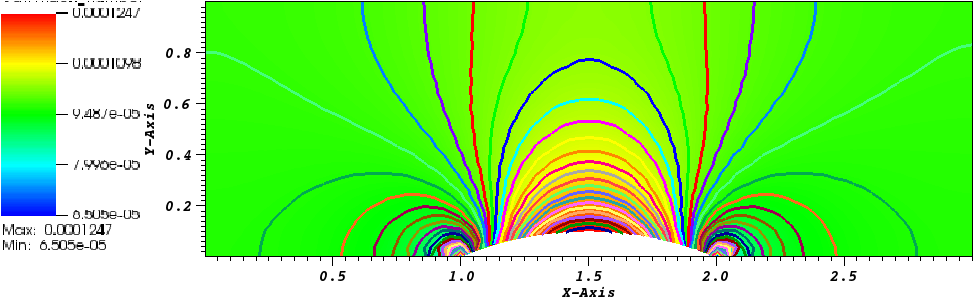
\includegraphics[width=\textwidth]{figures/Hump2D_mach_1em4.png}
                \caption{Mach $10^{-5}$}
                \label{fig:2d_hump_mach_0p0001}
        \end{figure}

        \begin{figure}[H]
                \centering
                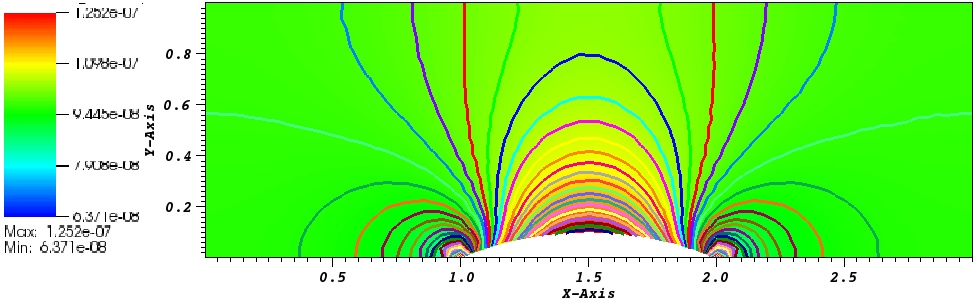
\includegraphics[width=\textwidth]{figures/Hump2D_mach_1em7.png}
                \caption{Mach $10^{-7}$}
                \label{fig:2d_hump_mach_0p0000001}
        \end{figure}
%        \caption{Iso-Mach lines for a 2-D flow over a circular bump (steady-state solution).}
%				\label{fig:2d_hump}
%\end{figure}
%
The results showed in \fig{fig:2d_hump_mach_0p01}, \fig{fig:2d_hump_mach_0p0001} and \fig{fig:2d_hump_mach_0p0000001} correspond to the low-Mach regime. The iso-Mach lines are drawn ranging from the minimum and the maximum values (provided in each legend) using 50 equally-spaced intervals. The steady-state solution is symmetric and does not depend on the value of the inlet Mach number, as expected in the incompressible limit. 

In \fig{fig:2d_hump_mach_0p7}, the steady-state numerical solution develops a shock: the compressibility effect are no longer negligible. The iso-Mach lines are also plotted with $50$ intervals and range from $0.4$ to $1.6$. The shock is well resolved and does not display any instabilities or spurious oscillations. \\
The results presented from \fig{fig:2d_hump_mach_0p01} through \fig{fig:2d_hump_mach_0p0000001} were obtained with the new definitions of the viscosity coefficients and illustrate the ability of the entropy viscosity method to correctly simulate several types of flows (subsonic and transonic flows) without tuning parameters.
%%%%%%%%%%%%%%%%%%%%%%%%%%%%%%%%%%%%%%%%%%%%%%%%%%%%%%%%%%%%%%%
%%%%%%%%%%%%%%%%%%%%%%%%%%%%%%%%%%%%%%%%%%%%%%%%%%%%%%%%%%%%%%%%%%%%%%%%%%%%%%%%%%%%%%%%%%%%%%%%%%%%
\section{Conclusions} \label{sec:ccl_sct3}
A new version of the entropy viscosity method valid for a wide range of Mach number and applied to the multi-D Euler equations with variable area was derived and presented. The definition of the viscosity coefficient is now consistent with the low Mach asymptotic limit, does not require an analytical expression of the entropy function, and thus, could be used with any equation of state having a convex entropy. Tests were performed with the Ideal and Stiffened Gas equation of states. In $1$-D, convergence of the numerical solution (either smooth or with shocks) to the exact solution was demonstrated by computing the convergence rates of the L$1$ and L$2$ norms of the error for flows in convergence-divergent nozzle and a straight pipe. $2$-D simulations were also performed for both subsonic and supersonic flows, and various geometries: the entropy viscosity method behaves well for a wide range of Mach number. The numerical results obtained for a flow over a circular bump (subsonic and transonic flows) illustrates the capabilities of the method to adapt to the flow type. \\
As future work, the entropy viscosity method will be extended to the $1$-D seven equations model \cite{SEM}. This two-phase flow system of equations is a good candidate for two reasons: it is unconditionally hyperbolic and degenerates to the multi-D Euler equations when one phase disappears.